%\documentclass{beamer}
% Uncomment the following line (and comment the one above) to get a PDF suitable
% for the website (i.e., no pauses).
\documentclass[handout]{beamer}
\mode<presentation>

{
  \usetheme{default}
  \usecolortheme{default}
  \usefonttheme{default}
  \setbeamertemplate{navigation symbols}{}
  \setbeamertemplate{caption}[numbered]
}

\usepackage{textcomp}
\usepackage{lmodern}
\usepackage[T1]{fontenc}
\usepackage[utf8]{inputenc}
\usepackage{dsfont}
\usepackage{exscale}
\usepackage[square,numbers]{natbib}     % better references
\usepackage[ruled]{algorithm2e} % must be loaded after natbib
\usepackage{dsfont}
\usepackage{mdwlist}
\usepackage{amsmath}
\usepackage{booktabs}
\usepackage{subfigure}
\usepackage{xspace}
\usepackage{pifont} % ding chars
\usepackage[export]{adjustbox}
\usepackage{xfrac} % sfrac
\usepackage{silence}
\WarningFilter{latexfont}{Font shape}

\definecolor{MyBlue}{rgb}{0.2,0.2,0.7}
\newcommand{\inblue}[1]{{\color{MyBlue}#1}}

\usetheme[height=0pt]{Rochester}
%\useoutertheme[footline=empty]{miniframes}
\useinnertheme{circles}
\setbeamercolor{math text}{fg=red}
\setbeamercolor{frametitle}{fg=blue}
\setbeamercolor{alerted text}{fg=blue}
\let\emph\alert
%\setbeamercolor{framesubtitle}{fg=blue}
\setbeamertemplate{frametitle}
{
\begin{centering}
\insertframetitle\par
\insertframesubtitle\par
\end{centering}
}
\beamertemplatenavigationsymbolsempty

%% slide number
\addtobeamertemplate{navigation symbols}{}{%
    \usebeamerfont{footline}%
    \usebeamercolor[fg]{footline}%
    \hspace{1em}%
    \insertframenumber/\inserttotalframenumber
}
\setbeamertemplate{caption}{\raggedright\insertcaption\par} % remove "Figure" in captions

\AtBeginSection[]{
  \begin{frame}
  \vfill
  \centering
  \begin{beamercolorbox}[sep=8pt,center,shadow=true,rounded=true]{title}
    \usebeamerfont{title}\insertsectionhead\par%
  \end{beamercolorbox}
  \vfill
  \end{frame}
}

\AtBeginSubsection[]{
  \begin{frame}
  \vfill
  \centering
  \begin{beamercolorbox}[sep=8pt,center,shadow=true,rounded=true]{title}
    \usebeamerfont{title}\insertsubsectionhead\par%
  \end{beamercolorbox}
  \vfill
  \end{frame}
}

\newcommand{\purple}{\color{purple}}
\newcommand{\black}{\color{black}}
\newcommand{\green}{\color{green}}
\newcommand{\red}{\color{red}}

\newcommand{\cmark}{\text{\ding{51}}}%
\newcommand{\xmark}{\text{\ding{55}}}%

\newcommand*{\allsp}{\ensuremath{\mathbb{S}}\xspace}
\newcommand*{\Sam}{{\cal S}\xspace}
\newcommand*{\range}{\mathcal{R}\xspace}
\newcommand*{\expectation}{\mathbb{E}\xspace}
\newcommand*{\indicator}{\mathds{1}\xspace}
\newcommand*{\family}{{\cal F}\xspace}
\newcommand*{\domain}{{\cal D}\xspace}
\newcommand*{\Rade}{\mathsf{R}\xspace}
\newcommand*{\prob}{\pi\xspace}

%% high level macros
\newcommand*{\betw}{\ensuremath{\mathsf{b}}\xspace}
\newcommand*{\closeness}{\ensuremath{\mathsf{c}}\xspace}
\newcommand*{\tbetw}{\ensuremath{\tilde{\betw}}\xspace}
\newcommand{\dist}{\ensuremath{d}\xspace}
\newcommand{\dep}{\ensuremath{\delta}\xspace}
\newcommand{\paths}{\ensuremath{\sigma}\xspace}
\newcommand{\pred}{\ensuremath{P}\xspace}
\newcommand{\sssp}{\ensuremath{\textsc{sssp}}\xspace}
\newcommand{\apsp}{\ensuremath{\textsc{apsp}}\xspace}
\renewcommand{\dag}{\ensuremath{\textsc{dag}}\xspace} % no need for daggers
\newcommand{\spath}{\ensuremath{\mathcal{S}}\xspace}
\newcommand{\allspath}{\ensuremath{\mathbb{S}\xspace}}
\newcommand{\spdag}{\ensuremath{\allspath\dag}\xspace}
\newcommand{\neighbors}{\ensuremath{\Gamma}\xspace}

\newtheorem{Claim}{Claim}

\title{\texorpdfstring{Centrality Measures on Big Graphs:\\Exact, Approximated, and Distributed
    Algorithms}{Centrality Measures on Big Graphs: Exact, Approximated, and Distributed
Algorithms}}
\author[Bonchi, De Francisci Morales, Riondato]{\texorpdfstring{Francesco Bonchi\inst{1,2}\\ \and
  Gianmarco De Francisci Morales\inst{3}\\ \and Matteo
Riondato\inst{4}}{Francesco Bonchi, Gianmarco De Francisci Morales, and Matteo
Riondato}}
\date[WWW'16]{WWW'16 -- Montr\'eal, April 11--15, 2016}
  \institute[ISI, Qatar Computing Research Institute, Two Sigma]{
  \inst{1} ISI Foundation, Turin (Italy)
  \and
  \inst{2} Eurecat, Technological Center of Catalonia, Barcelona (Spain)
  \and
  \inst{3} Qatar Computing Research Institute, Doha (Qatar)
  \and
  \inst{4} Two Sigma Investments, NYC (USA)
}

\begin{document}
\begin{frame}
  \titlepage
\end{frame}

%---------------------------------------------------------------------- SLIDE -

\frame{
  \frametitle{Acknowledgements}

\begin{itemize}
  \item Paolo Boldi
  \item Andreas Kaltenbrunner
  \item Evgenios M. Kornaropoulos
  \item Nicolas Kourtellis
  \item Eli Upfal
  \item Sebastiano Vigna
\end{itemize}

}

%---------------------------------------------------------------------- SLIDE -

\frame{
  \frametitle{Social network analysis}
\begin{itemize}
  \item Social network analysis is the study of social entities and their interactions and relationships.
 \pause \item The interactions and relationships can be represented with a network or graph,
  \begin{itemize}
  \pause  \item each vertex (or node) represents an actor and
  \pause  \item each link represents a relationship.
  \end{itemize}
 \pause \item From the network, we can study the properties of its structure, and the \alert{role}, \emph{position} and \emph{prestige} of each social entity.
\pause\item We can also find various kinds of sub-graphs, e.g., \emph{communities} formed by groups of entities.
\end{itemize}

}

%---------------------------------------------------------------------- SLIDE -

\frame{
  \frametitle{Centrality in networks}
\begin{itemize}
  \item Important or prominent actors are those that are linked or involved with other actors extensively.
\pause \item A person with extensive contacts (links) or communications with many other people in the organization is considered more important than a person with relatively fewer contacts.
\pause \item Central actor is one involved in many ties.
\pause \item \emph{Graph centrality} is a topic of uttermost importance in \emph{social sciences}.
\pause \item Also related to the problem of \emph{ranking} in the context of \emph{Web Search}:
\begin{itemize}
  \item Each webpage is a social actor and
  \item each hyperlink is an endorsement relationship.
  \item Centrality measures provide a query independent link-based score of \emph{importance} of a web page.
\end{itemize}
\end{itemize}

}


%---------------------------------------------------------------------- SLIDE -

\frame{
  \frametitle{History of centrality (in a nutshell)}
\begin{itemize}
	\pause\item first attempts in the late 1940s at M.I.T.~(Bavelas 1946), in the framework of communication patterns and
group collaboration;
	\pause\item in the following decades, various measures of centralities were proposed and employed by social scientists in a myriad of contexts (Bavelas 1951; Katz 1953;
Shaw 1954; Beauchamp 1965; Mackenzie 1966; Burgess 1969; Anthonisse 1971; Czapiel 1974...)
	\pause\item a new interest raised in the mid-90s with the advent of search engines: a ``reincarnation'' of centrality.
\end{itemize}


\pause Freeman (1979) observed:
	\begin{quotation}
	``several measures are often only vaguely related to
	the intuitive ideas they purport to index, and many are so complex that it is difficult
	or impossible to discover what, if anything, they are measuring''
	\end{quotation}
}

%---------------------------------------------------------------------- SLIDE -

\frame{
  \frametitle{Types of centralities}
Starting point: the central node of a star is the most important! Why?
\begin{enumerate}
  \pause\item the node with largest degree;
  \pause\item the node that is closest to the other nodes (e.g., that has the smallest average distance to other nodes);
  \pause\item the node through which most shortest paths pass;
  \pause\item the node with the largest number of incoming paths of length $k$, for every $k$;
  \pause\item the node that maximizes the dominant eigenvector of the graph matrix;
  \pause\item the node with highest probability in the stationary distribution of the natural random walk on the graph.
\end{enumerate}
\pause These observations lead to corresponding competing views of centrality.
}

%---------------------------------------------------------------------- SLIDE -

\frame{
  \frametitle{Types of centralities}
This observation leads to the following classes of indices of centrality:
\begin{enumerate}
  \pause\item measures based on distances [degree, closeness, Lin's index];
  \pause\item measures based on paths [betweenness, Katz's index];
  \pause\item spectral measures [dominant eigenvector, Seeley's index, PageRank, HITS, SALSA].
\end{enumerate}

\medskip

\pause The last two classes  are largely the same,
(even if that wasn't fully understood for a long time).

}

%---------------------------------------------------------------------- SLIDE -
\frame{
  \frametitle{Geometric centralities}
  \begin{itemize}
    \pause\item \emph{degree} (folklore): $c_{\mathrm{deg}}(x)=d^-(x)$
    \pause\item \emph{closeness} (Bavelas, 1950):
    $c_{\mathrm{clos}}(x)=\frac1{\sum_y d(y,x)}$
    \pause\item \emph{Lin} (Lin, 1976):
    $c_{\mathrm{Lin}}(x)=\frac{c(x)^2}{\sum_y d(y,x)}$ where $c(x)$ is the
    number of nodes that are co-reachable from $x$
 	\pause\item \emph{harmonic} (Boldi, Vigna, 2013)
 	$c_{\mathrm{harm}}(x)=\sum_{y\neq x}\frac1{d(y,x)}$
  \end{itemize}
}

%---------------------------------------------------------------------- SLIDE -
\frame{
  \frametitle{Path-based centralities}
  \begin{itemize}
    \pause\item \emph{betweenness} (Anthonisse, 1971):
    $c_{\mathrm{bet}}(x)=\sum_{y,z \neq x,\sigma_{yz}\neq 0}
    \frac{\sigma_{yz}(x)}{\sigma_{yz}}$ where $\sigma_{yz}$ is the number of
    shortest paths $y \to z$, and $\sigma_{yz}(x)$ is the number of such paths
    passing through $x$
    \pause\item \emph{Katz} (Katz, 1951):
    $c_{\mathrm{Katz}}(x)=\sum_{t\geq 0} \beta^t p_t(x)$ where $p_t(x)$ is the
    number of paths of length $t$ ending in $x$, and $\beta$ is a parameter
    ($\beta<1/\rho$)
  \end{itemize}
}

%---------------------------------------------------------------------- SLIDE -
\frame{
  \frametitle{Spectral centralities}
  \begin{itemize}
    \item \emph{dominant} (Wei, 1953):
    $c_{\mathrm{dom}}(x)$ is the dominant (right) eigenvector of $G$
    \item \emph{Seeley} (Seeley, 1949):
    $c_{\mathrm{Seeley}}(x)$ is the dominant (left) eigenvector of $G_r$
    \item \emph{PageRank} (Brin, Page \emph{et al.}, 1999):
    $c_{\mathrm{PR}}(x)$ is the dominant (left) eigenvector of $\alpha
    G_r+(1-\alpha) \mathbf{1}^T\mathbf{1}/n$ (where $\alpha<1$)
    \item \emph{HITS} (Kleinberg, 1997):
    $c_{\mathrm{HITS}}(x)$ is the dominant (left) eigenvector of $G^TG$
    \item \emph{SALSA} (Lempel, Moran, 2001):
    $c_{\mathrm{SALSA}}(x)$ is the dominant (left) eigenvector of $G_c^TG_r$
  \end{itemize}

  \medskip

 {\small Where  $G$ denotes the adjacency matrix of the graph, $G_r$ is the the adjacency matrix normalized by row, and $G_c$ is the adjacency matrix normalized by column.}
}


%---------------------------------------------------------------------- SLIDE -
\section{Closeness and Betweenness}

%---------------------------------------------------------------------- SLIDE -
\frame{
\frametitle{Closeness centrality}

Motivation
 \begin{itemize}
 \item Measures the ability to quickly access or pass information through the network.
\end{itemize}

Definition:
 \begin{itemize}
\item closeness centrality $C(i)$ of a  user $i$
$$
C(i)=1/\sum_{y\neq i \in V}d(y,i).
$$
%\item \footnotesize
\item $d(y,i)$ is the  length of shortest path
between nodes {\it y} and {\it i}.
\item The closeness of a node is defined as the inverse of the sum of the shortest distances between the node and all other nodes of the network.
\end{itemize}
}



%---------------------------------------------------------------------- SLIDE -
\frame{
\frametitle{Betweenness centrality}
Motivation
 \begin{itemize}
 \item Measures the frequency of a user in appearing in the shortest
   paths between two other users.
\end{itemize}

   \begin{columns}[T]
    \begin{column}{55mm}
Definition:
 \begin{itemize}
 \item  betweenness centrality $C_B(i)$ of a  user $i$
$
C_B(i)=\sum_{\substack{s\neq i\neq t \in V\\s\neq t}}
\frac{\sigma_{st}(i)}{\sigma_{st}}
$
\item[\footnotesize $\sigma_{st}$]  number of different shortest paths
between nodes {\it s} \& {\it t}
\item[\footnotesize $\sigma_{st}(i)$] how many of them pass over node
  {\it i}
\end{itemize}
   \end{column}
    \begin{column}{45mm}
  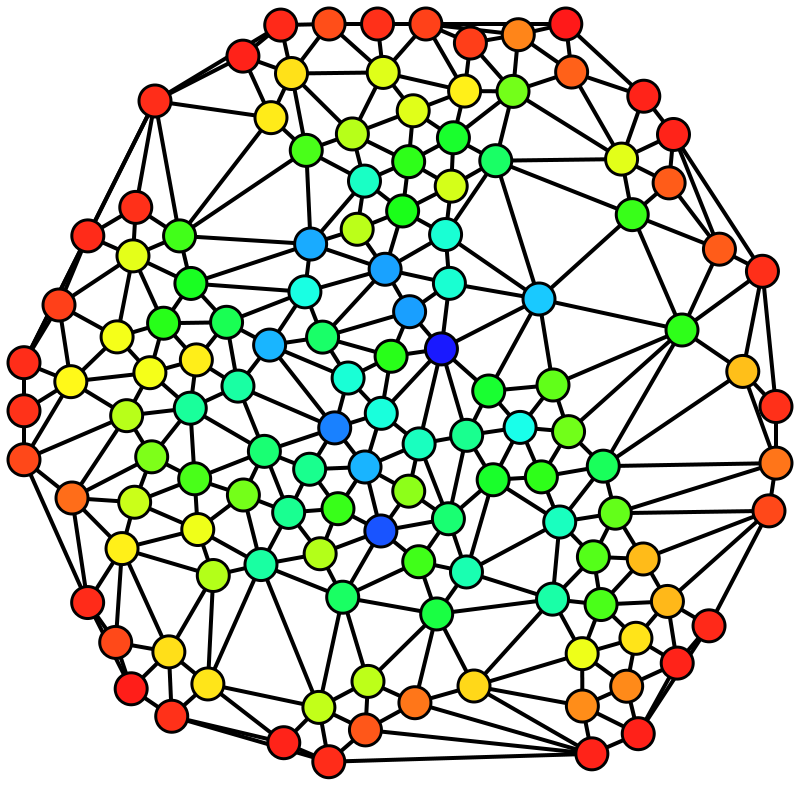
\includegraphics[width=42mm]{fig/Graph_betweenness.png}
\\ \hspace{10mm} \tiny{Example retrieved from  Wikipedia}
    \end{column}
  \end{columns}
}

%---------------------------------------------------------------------- SLIDE -
\frame{
\frametitle{Betweenness centrality}
\begin{itemize}
  \item Can be defined also for edges (similarly to nodes)
  \item Edges with high betweenness are what the sociologists call \emph{``weak ties''}. They tends to be the \emph{bridge} between two communities.
\end{itemize}

   \begin{columns}[T]
\begin{column}{60mm}
\emph{The strength of weak ties (Granovetter 1973)}
\begin{small}
\begin{itemize}
\item Dissemination and coordination dynamics are influenced by links established to nodes of different communities.
\item The importance of these links has become more and more with the rise of social networks and professional networking platforms.
\end{itemize}
\end{small}
   \end{column}
  \hspace{-16mm}\begin{column}{40mm}
 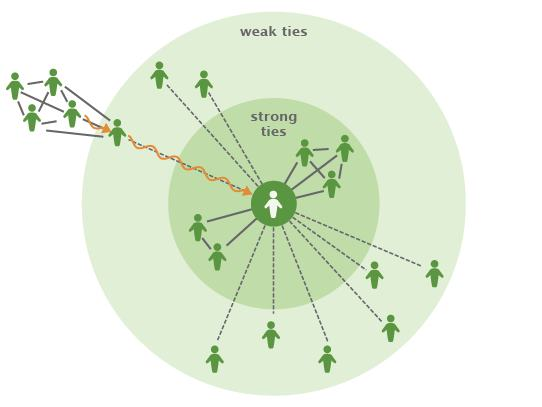
\includegraphics[width=62mm]{fig/weak_ties.png}
    \end{column}
  \end{columns}
}

%---------------------------------------------------------------------- SLIDE -
\frame{
\frametitle{Weak ties}
(Bakshy et al. 2012)
\begin{itemize}
\item
Weak links have a greater potential to expose links to new  contacts that otherwise would not have been discovered.
\end{itemize}

\begin{center}
 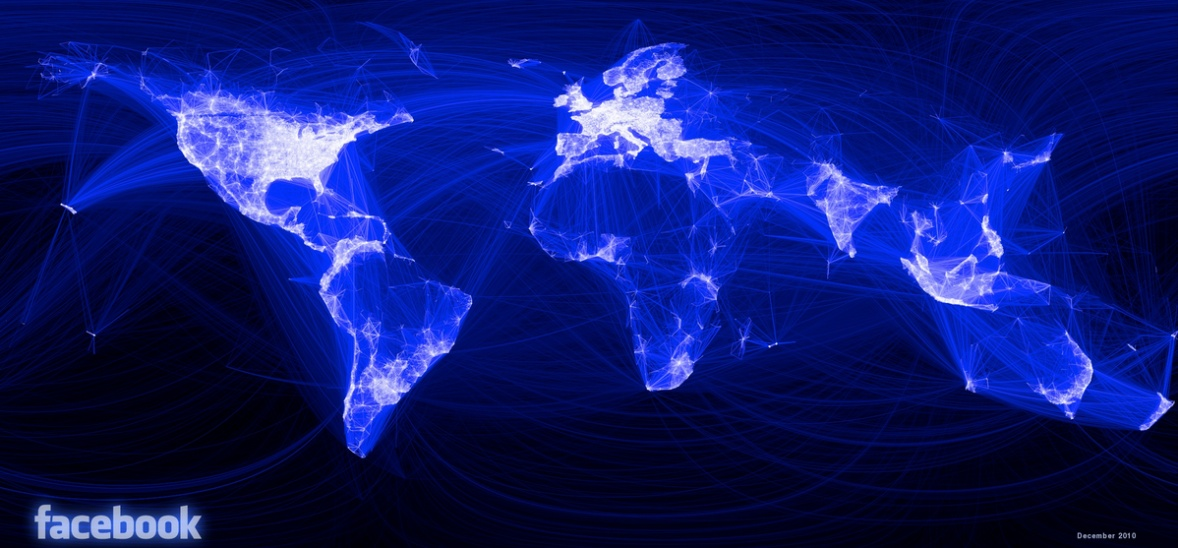
\includegraphics[width=70mm]{fig/facebook_graph.png}
 \end{center}
}

%---------------------------------------------------------------------- SLIDE -
\frame{
\frametitle{Weak ties}
(Grabowicz et al. 2012)
\begin{itemize}
\item Personal interactions are more likely to occur in internal links within communities (strong links)
 \item Events or new information is propagated faster by intermediate links (weak links).
\end{itemize}

\medskip

 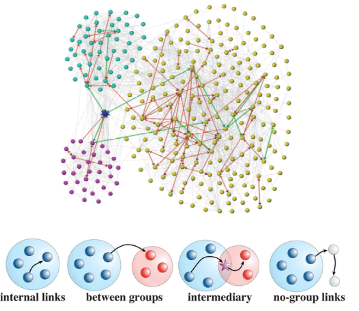
\includegraphics[width=50mm]{fig/weak_ties2.png}
 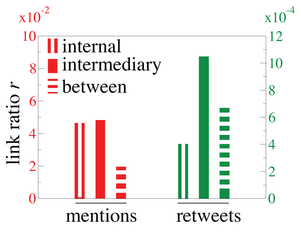
\includegraphics[width=50mm]{fig/weak_ties3.png}
}

%---------------------------------------------------------------------- SLIDE -
\frame{
\frametitle{Girvan-Newman algorithm for community detection (Girvan and Newman 2002)}
Hierarchical divisive clustering obtained by \emph{recursively removing the ``weakest tie''}.

\begin{enumerate}
  \item Compute edge betweenness centrality of all edges;
  \item Remove the edge with the highest betweenness centrality;
  \item Repeat from 1.
\end{enumerate}

\medskip
\centering
 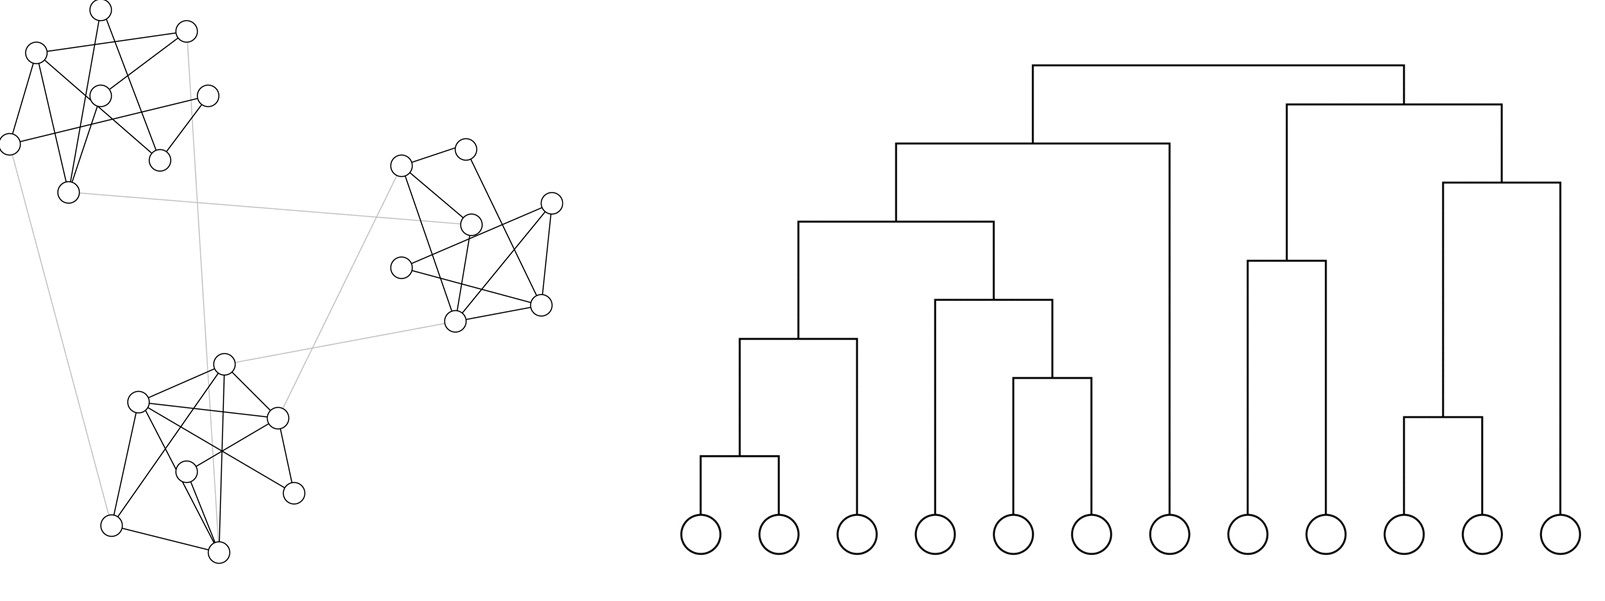
\includegraphics[width=82mm]{fig/gn.png}
}




%---------------------------------------------------------------------- SLIDE -
\frame{
\frametitle{Comparison}
\begin{block}{Which node is the most central?}
 \begin{itemize}
 \item for Degree Centrality:
 \item for Closeness Centrality:
 \item for Betweenness Centrality:
\end{itemize}
\end{block}
\centering
   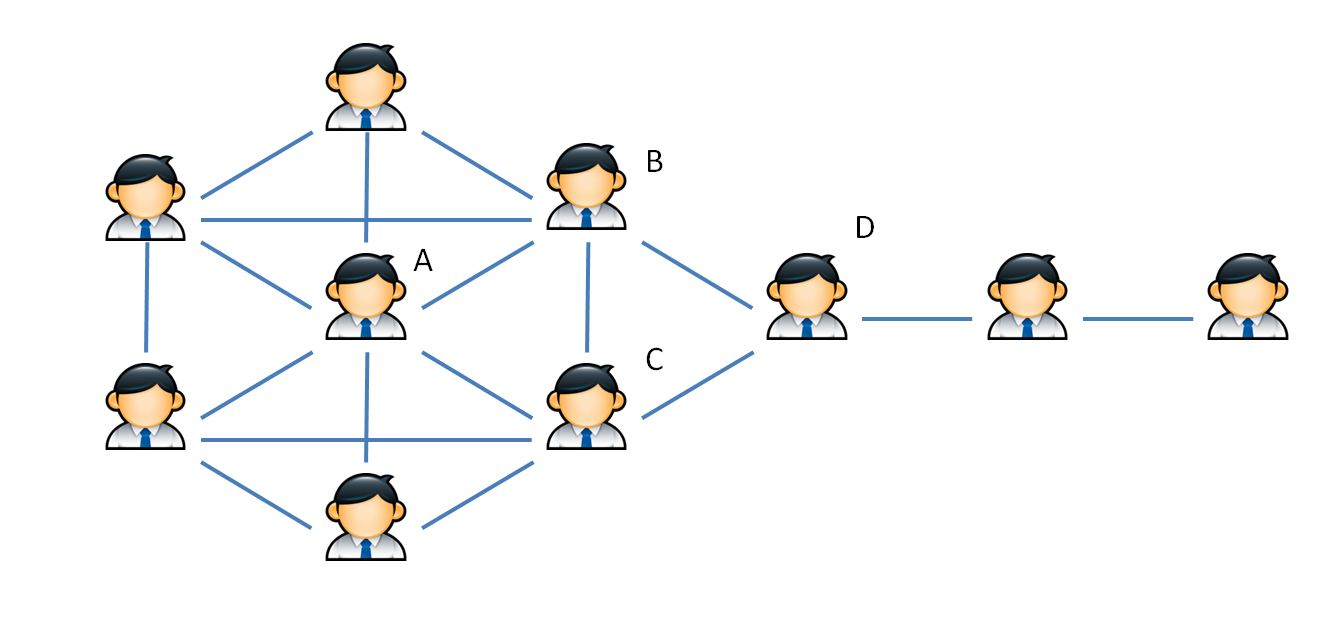
\includegraphics[width=100mm]{fig/centrality_comparison.png}
}

\frame{
\frametitle{Comparison}
\begin{block}{Which node is the most central?}
 \begin{itemize}
 \item for Degree Centrality:  {\color{blue}  user A}
 \item for Closeness Centrality:
 \item for Betweenness Centrality:
\end{itemize}
\end{block}
\centering
   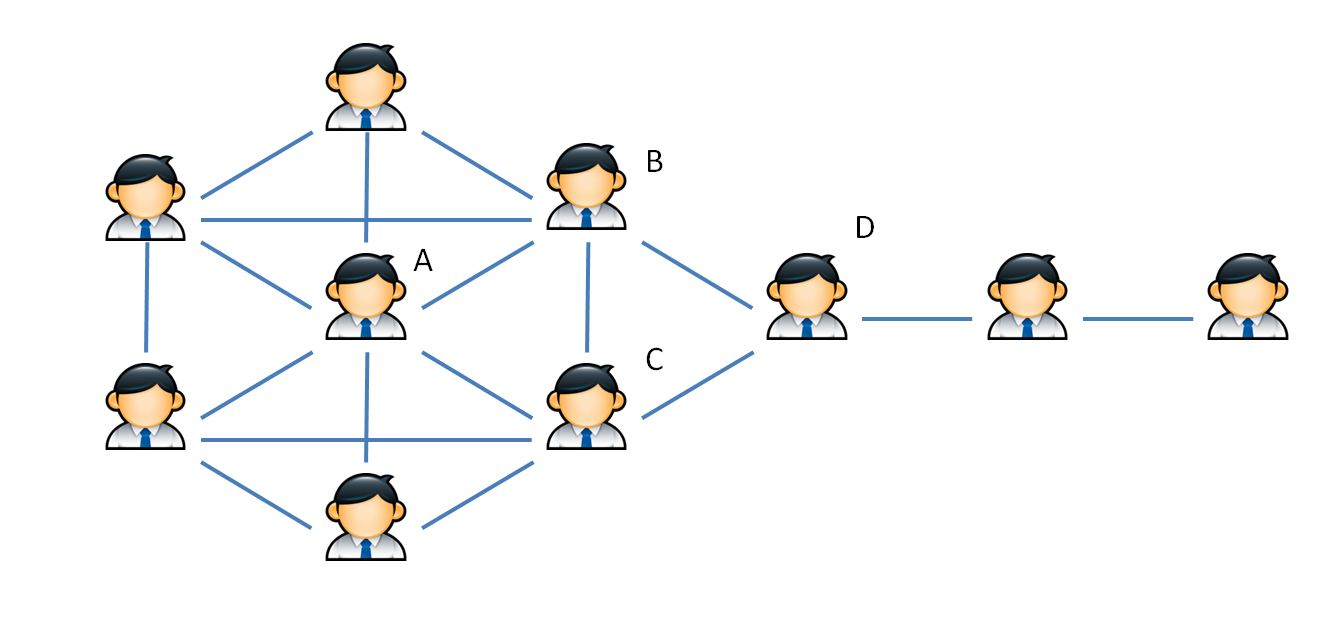
\includegraphics[width=100mm]{fig/centrality_comparison.png}
}

\frame{
\frametitle{Comparison}
\begin{block}{Which node is the most central?}
 \begin{itemize}
 \item for Degree Centrality: {\color{blue}  user A}
 \item for Closeness Centrality: {\color{blue}  users B and C}
 \item for Betweenness Centrality:
\end{itemize}
\end{block}
\centering
   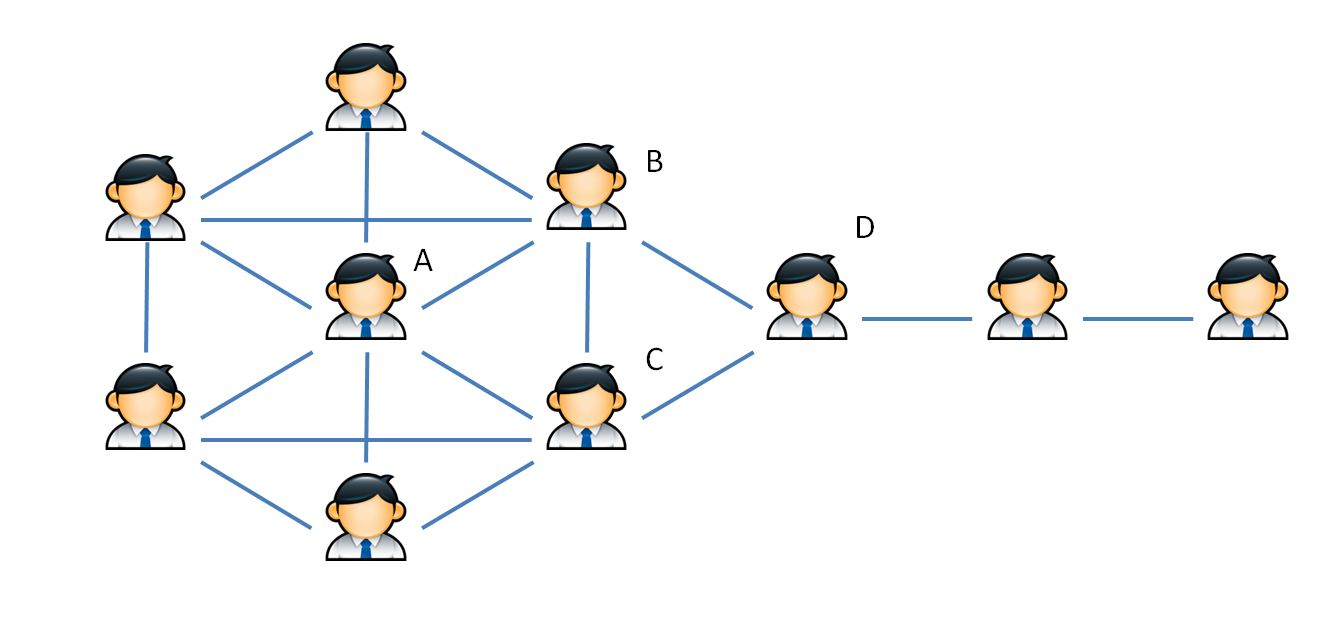
\includegraphics[width=100mm]{fig/centrality_comparison.png}
}

\frame{
\frametitle{Comparison}
\begin{block}{Which node is the most central?}
 \begin{itemize}
 \item for Degree Centrality: {\color{blue}  user A}
 \item for Closeness Centrality: {\color{blue}  users B and C}
 \item for Betweenness Centrality: {\color{blue}  user D}
\end{itemize}
\end{block}
\centering
   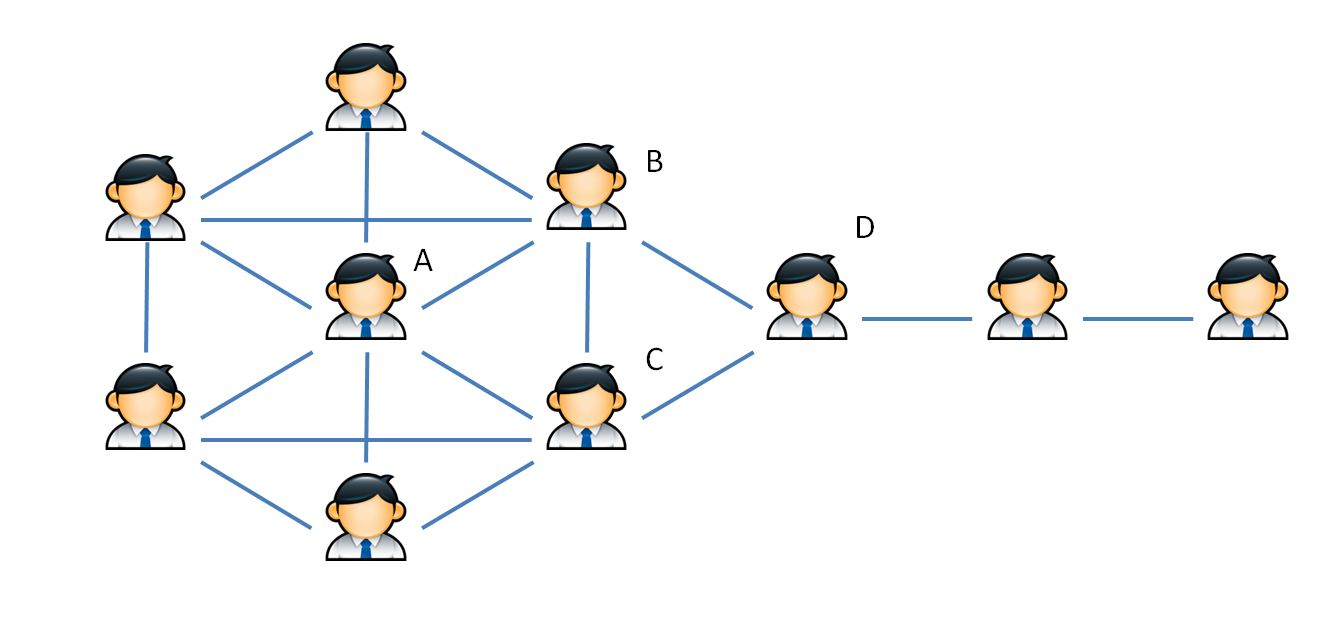
\includegraphics[width=100mm]{fig/centrality_comparison.png}
}

%---------------------------------------------------------------------- SLIDE -
\frame{
\frametitle{Visual Comparison}
 \begin{itemize}
 \item[A] Degree Centrality
 \item[B] Closeness Centrality
 \item[C] Betweenness Centrality
\end{itemize}

\centering
   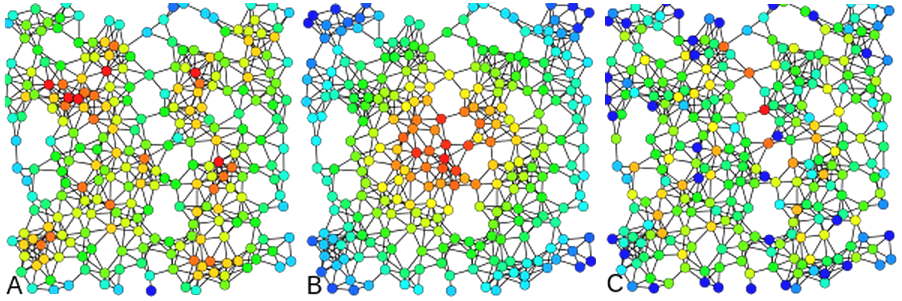
\includegraphics[width=100mm]{fig/centrality.png}
}




%---------------------------------------------------------------------- SLIDE -
\section{Axioms for centrality (Boldi and Vigna 2013)}




%---------------------------------------------------------------------- SLIDE -
\frame{
  \frametitle{Assessing}
  Is there a robust way to convince oneself that a certain centrality measure is
  better than another?

  Axiomatization\dots
  \begin{itemize}
    \pause\item \dots hard axioms (characterize a centrality measure completely)
    \pause\item \dots soft axioms (like the $T_i$ axioms for topological spaces)
  \end{itemize}
}

%---------------------------------------------------------------------- SLIDE -
\frame{
  \frametitle{Sensitivity to size}
  Idea: size matters!

   $S_{k,p}$ be the union of a $k$-clique and a $p$-cycle.
  \begin{itemize}
   \item if $k\to\infty$, every node of the clique becomes ultimately
    strictly more important than every node of the cycle
  \item if $p\to\infty$, every node of the cycle becomes ultimately
    strictly more important than every node of the clique
  \end{itemize}

  \medskip
  \centering
 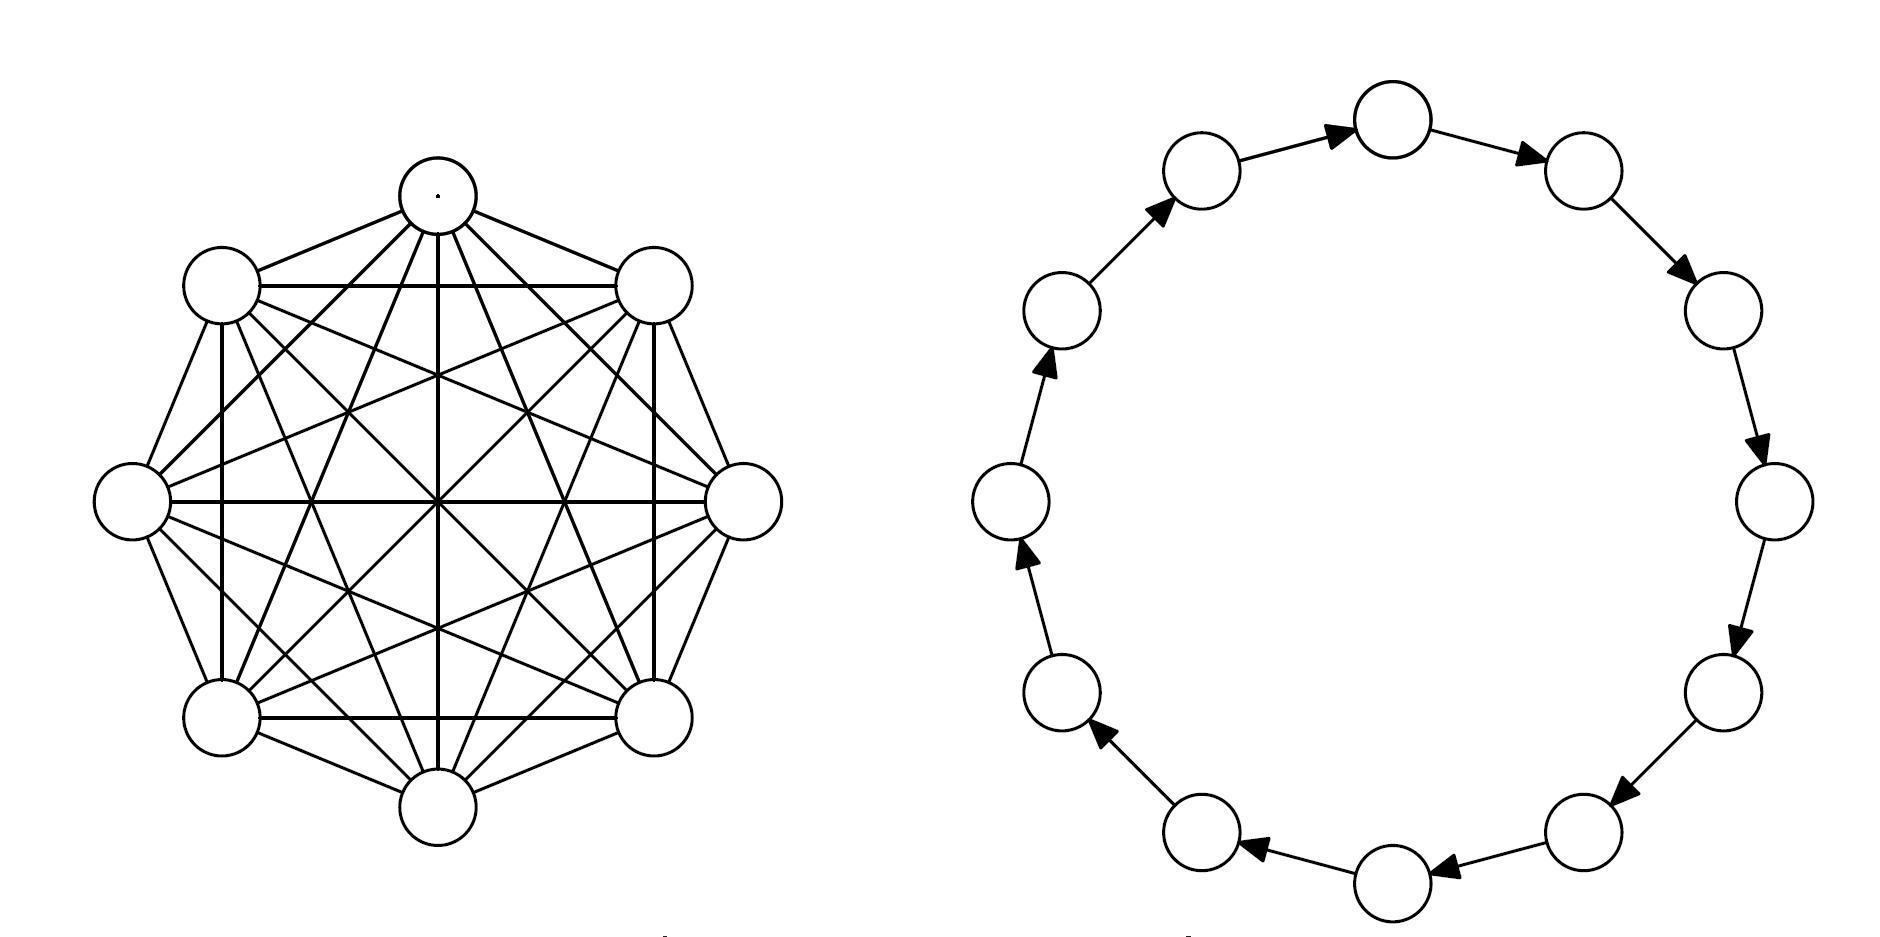
\includegraphics[width=82mm]{fig/sts.png}
}

%---------------------------------------------------------------------- SLIDE -
\frame{
  \frametitle{Sensitivity to density}
  Idea: density matters!

 $D_{k,p}$ be made by a $k$-clique and a $p$-cycle connected by a single
  bidirectional bridge:
  \begin{itemize}
    \item if $k\to\infty$, the node on the clique-side of the bridge
    becomes more important than the node on the cycle-side.
  \end{itemize}

    \medskip
  \centering
 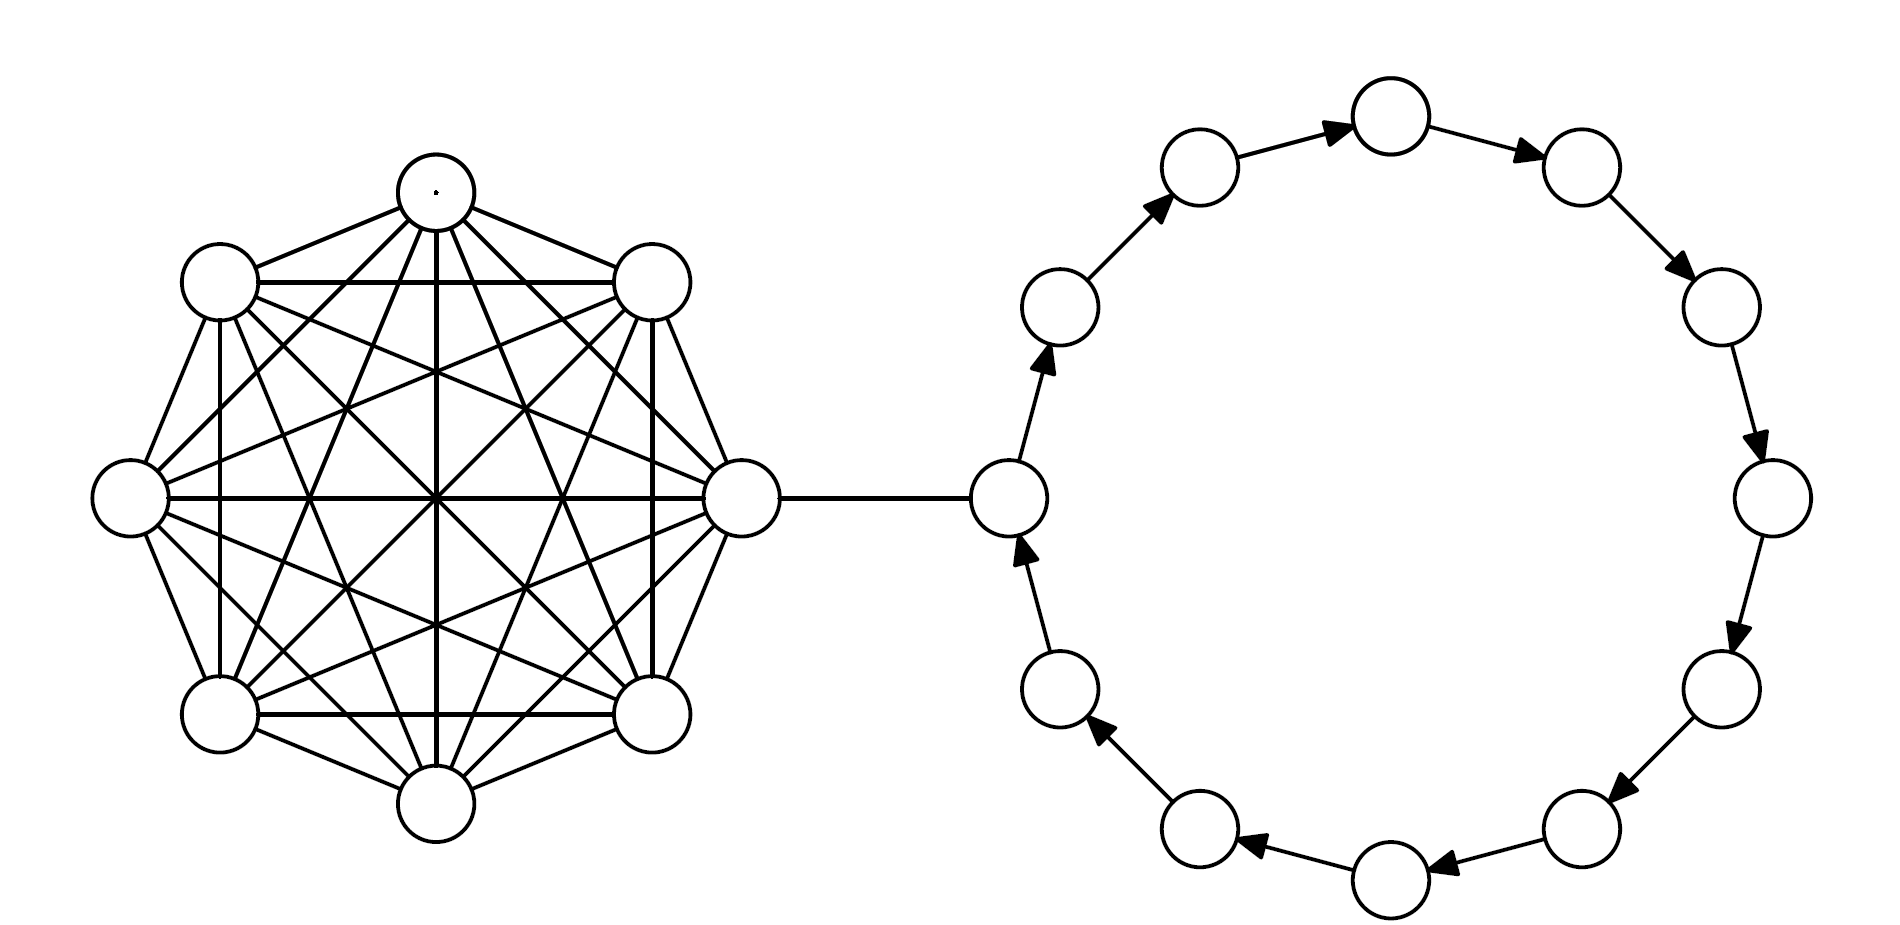
\includegraphics[width=82mm]{fig/std.png}
}

%---------------------------------------------------------------------- SLIDE -
\frame{
  \frametitle{Score monotonicity}
  Adding an arc $x \to y$ strictly increases the score of $y$.

  \smallskip
  \pause {\bf Doesn't say anything about the score of other nodes!}
}

%---------------------------------------------------------------------- SLIDE -
\frame{
  \frametitle{Rank monotonicity}
  Adding an arc $x \to y$\dots
  \begin{itemize}
    \pause\item if $y$ used to dominate $z$, then the same holds after adding
    the arc
    \pause\item if $y$ had the same score as $z$, then the same holds after
    adding the arc
	\pause\item {\bf strict variant: } if $y$ had the same score as $z$, then $y$
	dominates $z$ after adding the arc
  \end{itemize}
}

%---------------------------------------------------------------------- SLIDE -
\frame{
  \frametitle{Rank monotonicity}
\begin{table}
\renewcommand{\arraystretch}{1.2}
\begin{minipage}{\textwidth}
\centering
\begin{tabular}{l|c|c|c|c|c|c}
\multicolumn{1}{c|}{}&\multicolumn{4}{c|}{Monotonicity}&\multicolumn{2}{c}{Other axioms}\\
\multicolumn{1}{c|}{}&\multicolumn{2}{c|}{General}&\multicolumn{2}{c|}{Strongly connected}&\multicolumn{2}{c}{}\\
Centrality & Score & Rank & Score & Rank & Size & Density
\\
\hline
Harmonic & yes  & yes* & yes & yes* & yes & yes \\
Degree  & yes & yes* & yes & yes* & only $k$ & yes \\
Katz & yes & yes*& yes & yes* & only $k$ & yes \\
PageRank &  yes & yes*& yes & yes* & no & yes \\
Seeley & no & no & yes & yes & no & yes \\
Closeness & no  & no & yes & yes & no & no \\
Lin & no & no & yes & yes & only $k$& no \\
Betweenness & no & no & no & no & only $p$ & no \\
Dominant & no & no &? &? & only $k$ & yes \\
HITS & no & no & no &no & only $k$ &yes\\
SALSA & no & no & no &no & no & yes
\end{tabular}
\end{minipage}
\end{table}
}

%---------------------------------------------------------------------- SLIDE -
\frame{
  \frametitle{Kendall's $\tau$}

\begin{tabular}{c}
  Hollywood collaboration network\\
 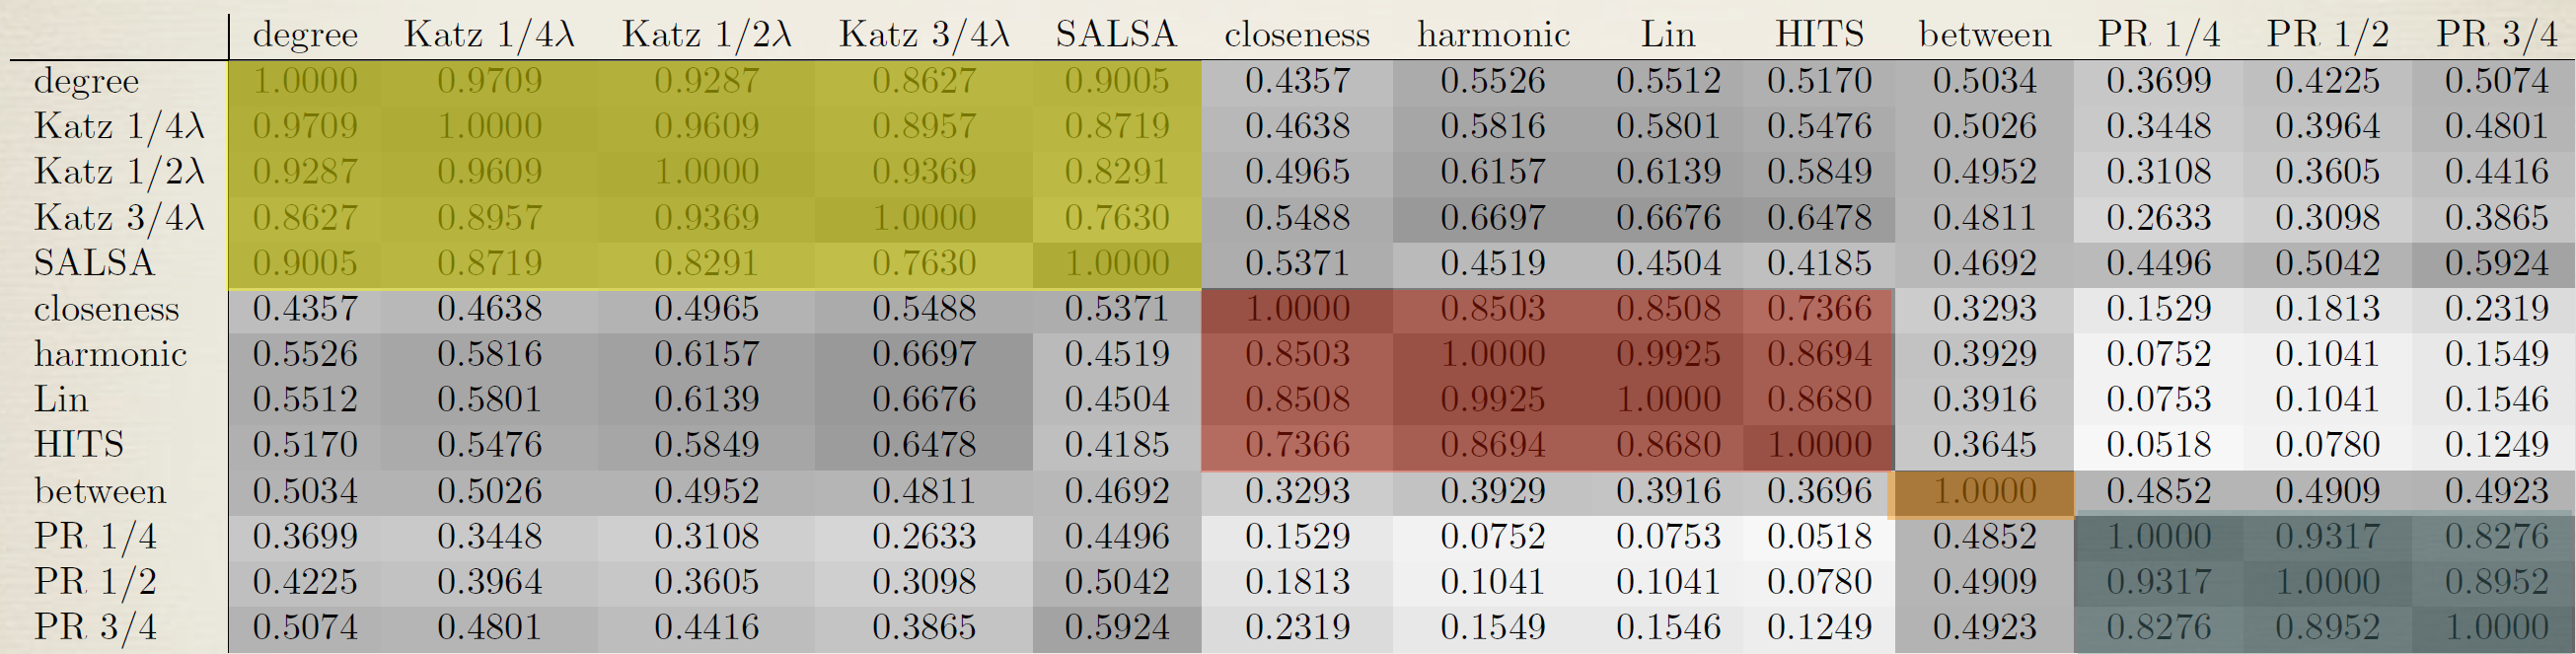
\includegraphics[width=\textwidth]{fig/kendall2.png}\\
 \medskip \\
  .uk (May 2007 snapshot)\\
 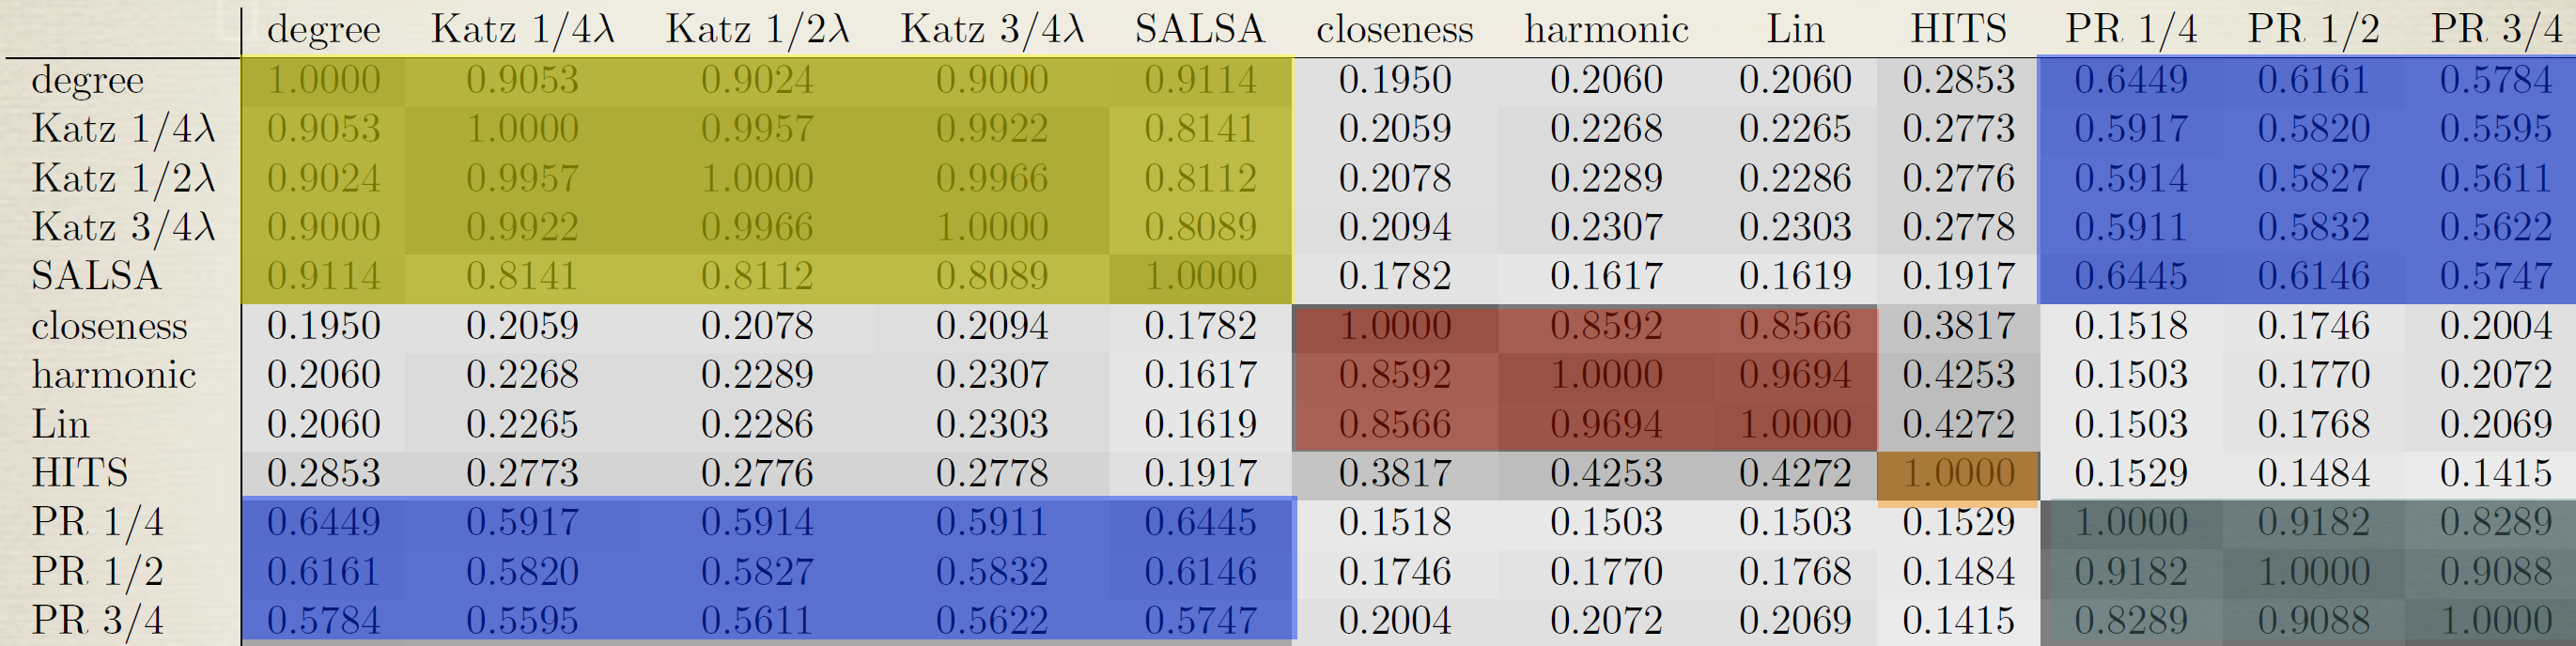
\includegraphics[width=\textwidth]{fig/kendal.png}\\
\end{tabular}
}

%---------------------------------------------------------------------- SLIDE -
\frame{
  \frametitle{Correlation}
\begin{itemize}
 \pause \item most geometric indices and HITS
are rather correlated to one another;
  \pause \item Katz, degree and SALSA are also
highly correlated;
  \pause \item PageRank stands alone in the first dataset, but it is correlated to degree, Katz, and SALSA in the second dataset;
  \pause \item Betweenness is not correlated to anything in the first dataset, and could not be computed in the second dataset due to the size of the graph (106M vertices).
\end{itemize}

}

% Contains
%   - Intro
%   - Overview of centrality measures
%   - Axioms for centrality
% !TEX root =  centrtutorial.tex

\section{Exact Algorithms}
\begin{frame}
  \frametitle{Outline}
  \begin{enumerate}
    \item Exact algorithms for static graphs
      \begin{enumerate}
        \item the standard algorithm for closeness
        \item the standard algorithm for betweenness
        \item a faster betweenness algorithm through shattering and compression
        \item a GPU-Based algorithm for betweenness
      \end{enumerate}
    \item Exact algorithms for dynamic graphs
      \begin{enumerate}
        \item a dynamic algorithm for closeness
        \item four dynamic algorithms for betweenness
        \item a parallel streaming algorithm for betweenness
      \end{enumerate}
  \end{enumerate}
\end{frame}

\subsection{Exact Algorithms for Static Graphs}

\begin{frame}
  \centering
  \vfill
  {\huge Exact Algorithm for Closeness Centrality}
  \vfill
  {\Large(folklore)}
  \vfill
\end{frame}

\begin{frame}
  \frametitle{Exact Algorithm for Closeness}
    \vfill
    Recall the definition:
    \[
      \closeness(x)=\frac{1}{\sum_{y\neq x}d(x,y)}
    \]
    \vfill
    \pause
    Fastest known algorithm for closeness: \emph{All-Pair-Shortest Paths}
    \begin{itemize}
      \item Runtime: $O(nm+n^2\log n)$
    \end{itemize}
    \vfill
    \pause
    Too slow for \emph{web-scale} graphs!
    \begin{itemize}
      \item Later we'll discuss an \emph{approximation algorithm}
    \end{itemize}
    \vfill
\end{frame}

\begin{frame}
  \centering
  \vfill
  {\huge A Faster Algorithm for Betweenness Centrality}
  \vfill
  {\Large U.~Brandes}
  \vfill
  {\large Journal of Mathematical Sociology (2001)}
  \vfill
\end{frame}

\begin{frame}
  \frametitle{Why {\red faster}?}
  \vfill
  Let's take a step back. Recall the definition
  \[
    \sum_{\substack{s\neq x\neq t \in V\\s\neq t}}\frac{\sigma_{st}(x)}{\sigma_{st}}
    \vspace{-10pt}
  \]
  \begin{itemize}
    \item $\sigma_{st}$: no.~of SPs from $s$ to $t$
    \item $\sigma_{st}(x)$: no.~of SPs from $s$ to $t$ that go through $x$
  \end{itemize}
  \pause
  We could:
  \begin{enumerate}
    \item obtain all the $\sigma_{st}$ and $\sigma_{st}(x)$ for all $x$, $s$,
      $t$ via APSP; and then
    \item perform the aggregation to obtain $\betw(x)$ for all $x$.
  \end{enumerate}
  \pause
  The first step takes $O(nm+n^2\log n)$, but the second step takes\ldots\pause
  $\Theta(n^3)$ (a sum of $O(n^2)$ terms for each of the $n$ vertices).
  \pause
  \vfill
  Brandes' algorithm interleaves the SP computation with the aggregation,
  achieving runtime $O(nm+n^2\log n)$\\
  \quad I.e., it is \emph{faster} than the APSP approach
\end{frame}

\begin{frame}
  \frametitle{Dependencies}
  Define: \emph{Dependency} of $s$ on $x$:
  \[
    \dep_s(v)=\sum_{t\neq s\neq v}\frac{\sigma_{st}(v)}{\sigma_{st}}
  \]
  Hence:
  \[
    \betw(v)=\sum_{s\neq v}\dep_s(v)
  \]
  \pause
  Brandes proved that $\delta_s(v)$ obeys a \emph{recursive relation}:
  \[
    \dep_s(v)=\sum_{w:v\in\pred_s(w)}\frac{\sigma_{sv}}{\sigma_{sw}}\left(1+\dep_s(w)\right)
  \]
  We can leverage this relation for efficient computation of betweenness.
\end{frame}

\begin{frame}
  \frametitle{Recursive relation}
  \begin{theorem}[Simpler form]
    If there is exactly one SP from $s$ to each $t$, then
    \[
      \dep_s(v)=\sum_{w: v\in\pred_s(w)}\left(1+\dep_s(w)\right)
    \]
  \end{theorem}
  \pause
  \emph{Proof sketch:}
  \begin{itemize}
    \item The SP DAG from $s$ is a tree;
    \item Fix $t$. $v$ is either on the single SP from $s$ to $t$ or not.
    \item $v$ lies on all and only the SPs to vertices $w$ for which $v$ is a
      predecessor (one SP for each $w$) and the SPs that these lie on. Hence the
      thesis.
  \end{itemize}
  \pause
  The general version must take into account that not all SPs from $s$ to $w$ go
  trough $v$.
\end{frame}

\begin{frame}
  \frametitle{Brandes' Algorithm}
  \begin{enumerate}
    \item Initialize $\dep_s(v)$ to $0$ for each $v,s$ and $\betw(w)$ to $0$ for
      each $w$.
    \item Iterate the following loop for each vertex $s$:
      \begin{enumerate}
        \item Run Dijkstra's algorithm from $s$, keeping track of $\sigma_{sv}$ for
          each encountered vertex $v$, and inserting the vertices in a max-heap $H$ by
          distance from $s$;
        \item While $H$ is not empty:
          \begin{enumerate}
            \item Pop the max vertex $t$ in $H$;
            \item For each $w\in\pred_s(t)$, increment $\dep_s(w)$ by
              $\frac{\sigma_{sw}}{\sigma_{st}}(1+\dep_s(t))$;
            \item Increment $\betw(t)$ by $\dep_s(t)$;
          \end{enumerate}
      \end{enumerate}
  \end{enumerate}
\end{frame}

\begin{frame}
  \centering
  \vfill
  {\huge Shattering and Compressing Networks for Betweenness Centrality}
  \vfill
  {\Large A.~E.~Sar\i y\"uce, E.~Saule, K.~Kaya, \"U.~V.~\c{C}ataly\"urek}
  \vfill
  {\large SDM '13: SIAM Conference on Data Mining}
  \vfill
\end{frame}

\begin{frame}
  \frametitle{Intuition}
  \emph{Observations:}
  \begin{itemize}
    \item There are vertices with predictable betweenness (e.g., 0, or equal to one
      of their neighbors). We can remove them from the graph (\emph{compression})
    \item Partitioning the (compressed) graph into small components allows for
      faster SP computation (\emph{shattering})
  \end{itemize}
  \pause
  \emph{Idea}:
  We can iteratively compress \& shatter until we can't reduce the graph any
  more.\\
  \qquad Only at this point we run (a modified) Brandes's algorithm and then
  aggregate the ``partial'' betweenness in different components.
\end{frame}

\begin{frame}
  \frametitle{Introductory definitions}
  \vfill
  \begin{itemize}
    \item Graph $G=(V,E)$
    \item \emph{Induced graph} by $V'\subseteq V$: $G_{V'}=(V', E'=V'\times V'\cap E)$
    \pause
    \item Neighborhood of a vertex $v$: $\neighbors(v)=\{u~:~(v,u)\in V\}$
    \pause
  \item \emph{Side vertex}: a vertex $v$ such that $G_{\neighbors(v)}$ is a clique
    \pause
  \item \emph{Identical vertices}: two vertices $u$ and $v$ such that either
      $\neighbors(u)\neighbors(v)$ or
      $\neighbors(u)\cup\{u\}=\neighbors(v)\cup\{v\}$
  \end{itemize}
  \vfill
\end{frame}


\begin{frame}
  \frametitle{Compression}
  \vfill
  Empirical / Intuitive observations
  \begin{itemize}
    \item if $v$ has degree $1$, then $\betw(v)=0$
    \item if $v$ is a side vertex, then $\betw(v)=0$
    \item if $u$ and $v$ are identical, then $\betw(v)=\betw(w)$
  \end{itemize}
  \pause
  \vfill
  \emph{Compression}:
  \begin{itemize}
    \item remove degree-1 vertices and side vertices; and
    \item merge identical vertices
  \end{itemize}
  \vfill
\end{frame}

\begin{frame}
  \frametitle{Shattering}
  \vfill
  \begin{itemize}
    \item \emph{Articulation vertex}: vertex $v$ whose deletion makes the graph disconnected
    \item \emph{Bridge edge:} an edge $e$ such that $G'=(V,E\setminus\{e\})$ has
      more components than $G$.
  \end{itemize}
  \pause
  \vfill
  \emph{Shattering}:
  \begin{itemize}
    \item remove bridge edges; and
    \item split articulation vertices in two copies, one per resulting component
  \end{itemize}
\end{frame}

\begin{frame}
  \frametitle{Example of shattering and compression}
  \begin{figure}
    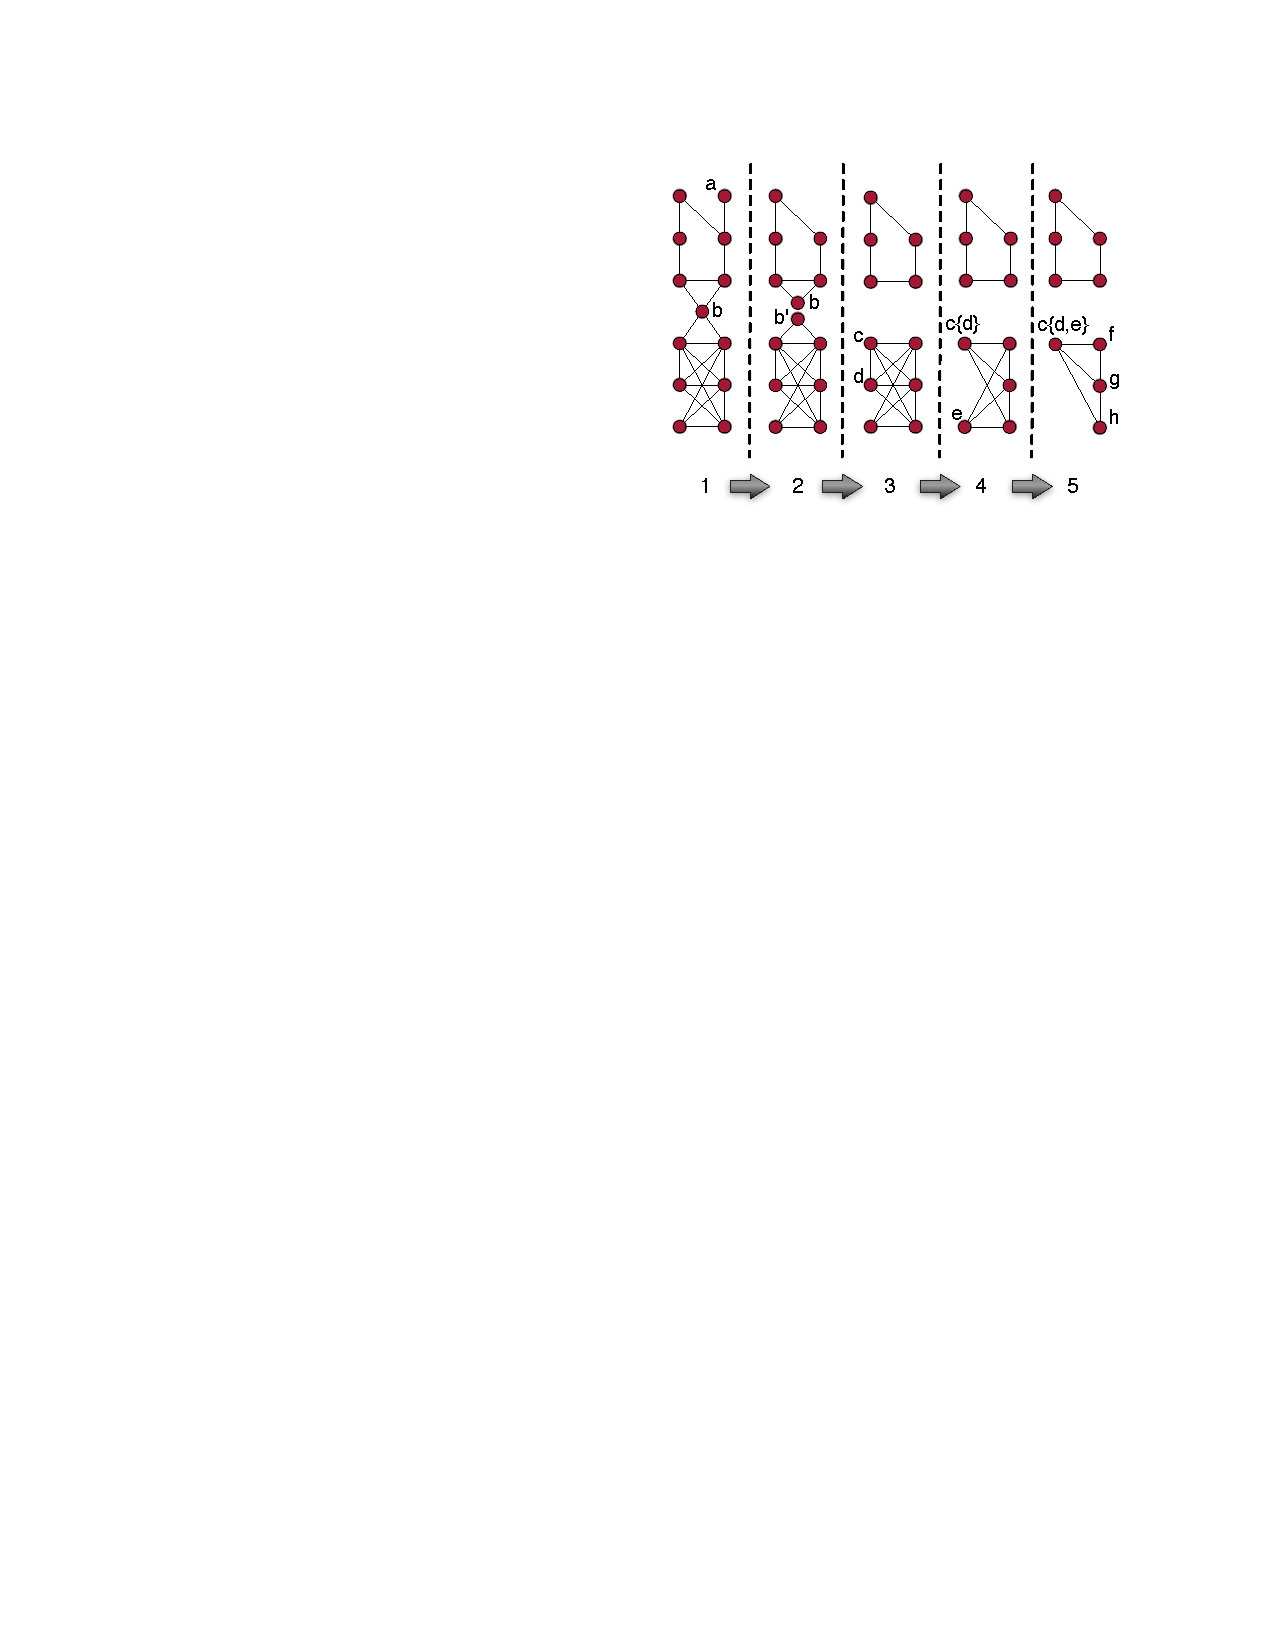
\includegraphics{figs/shatteringbadios.pdf}
  \end{figure}
\end{frame}

\begin{frame}
  \frametitle{Issues}
  There are issues to take care of when iteratively compressing \& shattering:
  \begin{block}{Example of issue}
    A vertex may have degree 1 only after we removed another vertex: we can't
    just remove and forget it, as its original betweenness was not 0.
  \end{block}
  \pause
  \begin{block}{Example of issue}
    When splitting an articulation vertex into component copies, we need to know,
    for each copies , how many vertices in other components are reachable through
    that vertex.
  \end{block}
  ... and more
\end{frame}

\begin{frame}
  \frametitle{Solution}
  (Sketch)
  \begin{itemize}
    \item When we remove a vertex $u$, one of its neighbors (or an identical vertex)
      $v$ is elected as the representative for $u$ (and for all vertices that $u$
      was a representative of.)
    \item We adjust the (current) values of $\betw(v)$ and $\betw(u)$ to
      appropriately take into account the removal of $u$\\
      \qquad the details are too hairy for a talk\ldots
    \item When splitting articulation vertices or removing bridges, similar
      adjustments take place.
    \item Brandes' algorithm is slightly modified to take the number of vertices
      that a vertex represents into consideration when computing the
      dependencies and the betweenness values.
  \end{itemize}
\end{frame}

\begin{frame}
  \frametitle{Speedup}
  ``org.'' is Brandes' algorithm, ``best'' is compress \& shatter
  \begin{figure}
    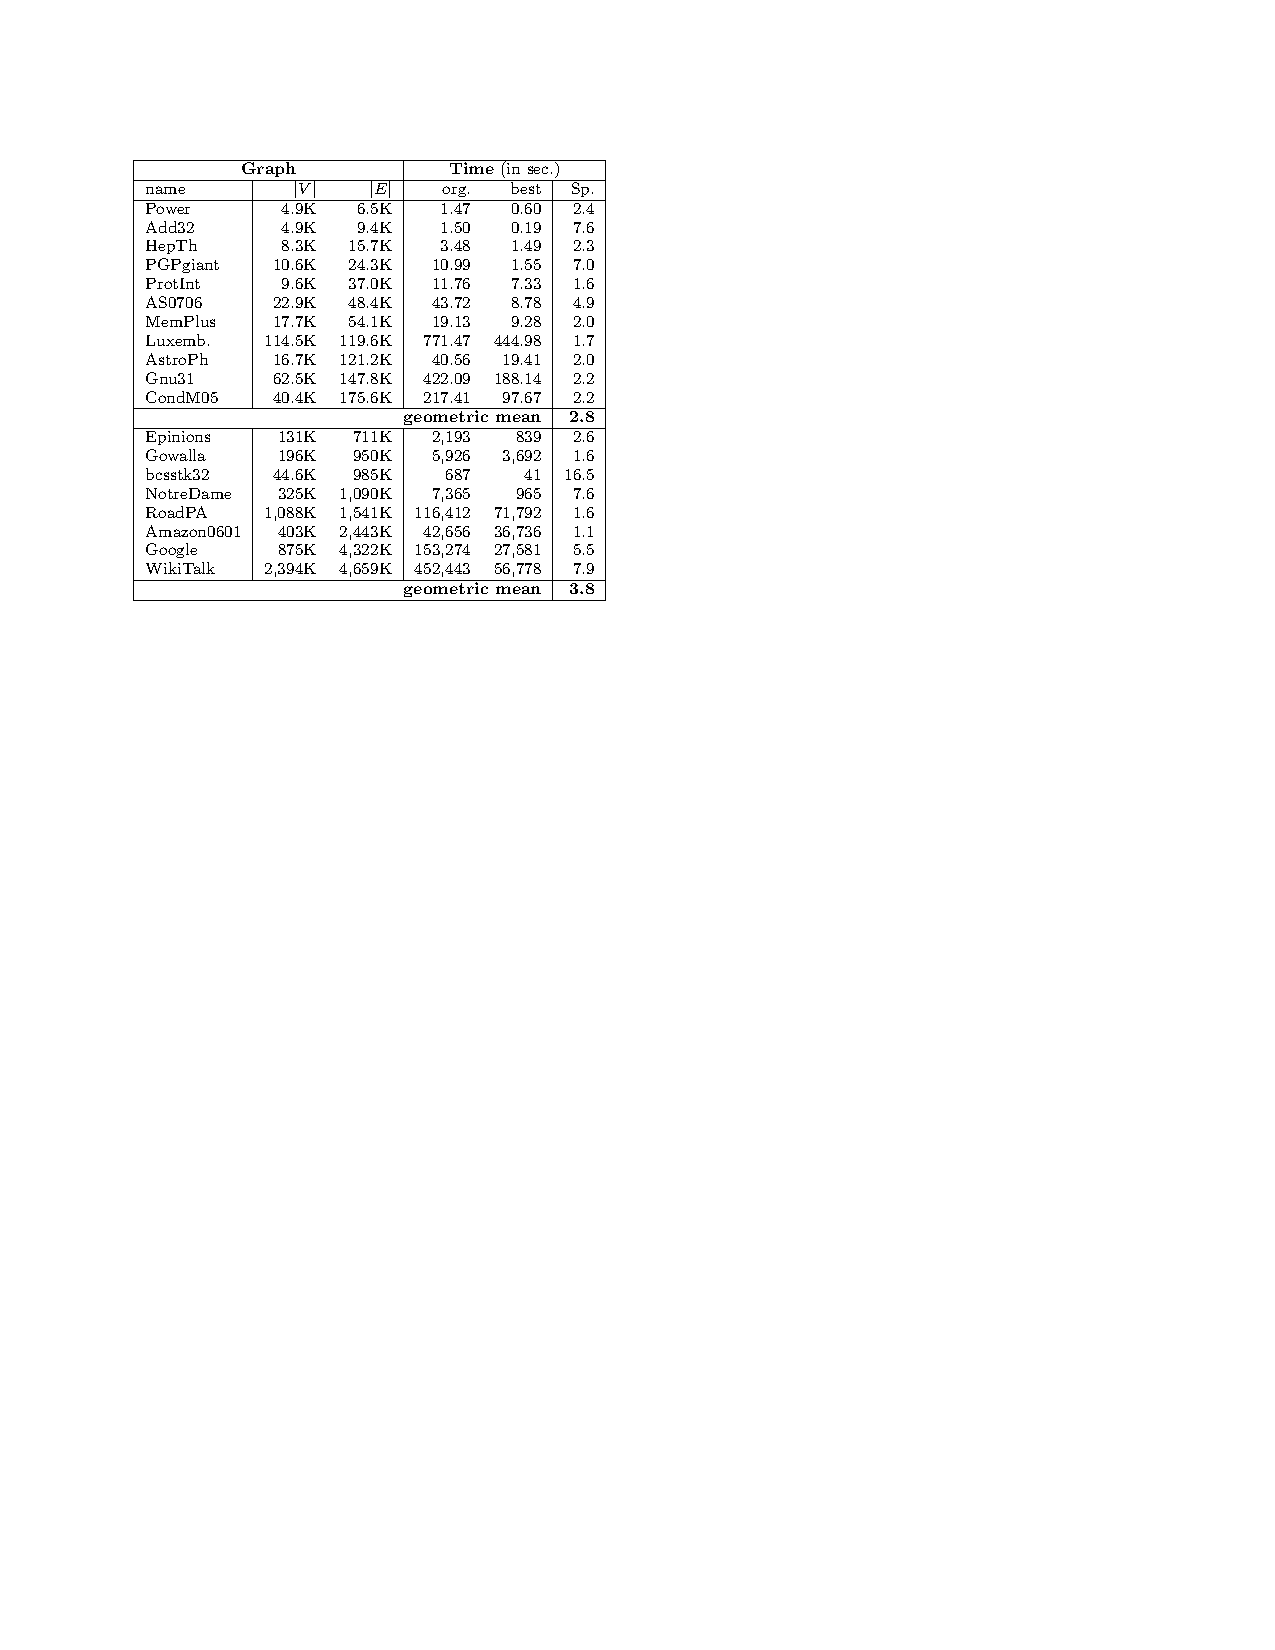
\includegraphics{figs/runtimebadios.pdf}
  \end{figure}
\end{frame}

\begin{frame}
  \frametitle{Composition of runtime}
  \begin{itemize}
    \item Preproc is the time needed to compress \& shatter, Phase 1 is SSSP,
      Phase 2 is aggregation
    \item Different column for different variants of the algorithm (e.g., only
      compression of 1-degree vertices, only shattering of edges)
    \item the lower the better
  \end{itemize}
  \begin{figure}
    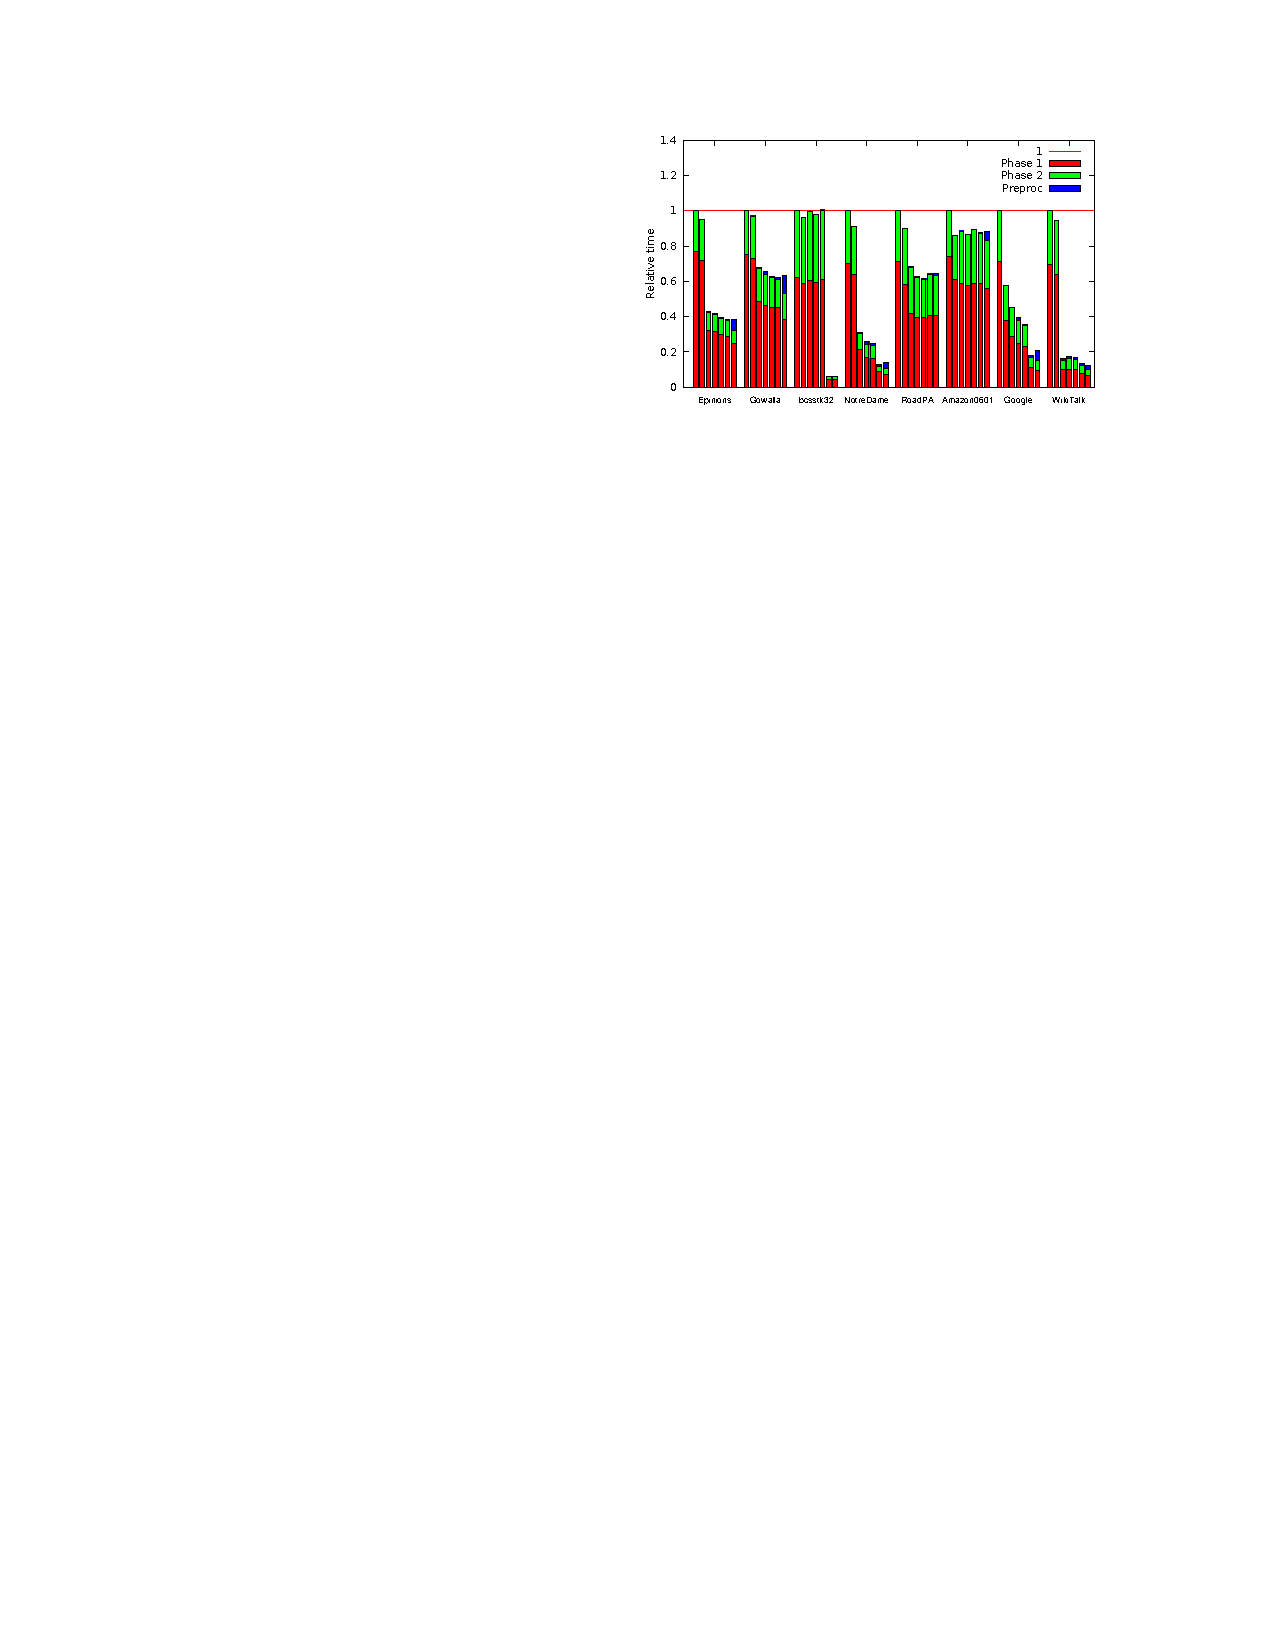
\includegraphics[width=0.9\textwidth]{figs/runtimesplitbadios.pdf}
  \end{figure}
\end{frame}

%\begin{frame}
%  \frametitle{A Divide-and-Conquer Algorithm for Betweenness Centrality}
%  \centering
%  \vfill
%  {\huge D.~Erd\H{o}s, V.~Ishakian, A.~Bestravros, E.~Terzi}
%  \vfill
%  {\large SIAM Data Mining Conference (2015)}
%\end{frame}

%% Sariyüce et al.
\begin{frame}
  \centering
  \vfill
  {\huge Betweenness Centrality on GPUs and Heterogeneous Architectures}
  \vfill
  {\Large A.~E.~Sar\i y\"uce, K.~Kaya, E.~Saule, \"U.~V.~\c{C}ataly\"urek}
  \vfill
  {\large GPGPU '13: Workshop on General Purpose Processing Using GPUs}
  \vfill
\end{frame}

\begin{frame}
  \frametitle{Parallelism}

  \begin{itemize}
    \item Fine grained: single concurrent BFS
    \item Only one copy of auxiliary data structures
    \item Synchronization needed
    \item Better for GPUs, which have small memory
  \end{itemize}
  \begin{itemize}
    \item Coarse grained: many independent BFSs
    \item Sources are independent, embarrassingly parallel
    \item More memory needed
    \item Better for CPUs, which have large memory
  \end{itemize}
\end{frame}

\begin{frame}
  \frametitle{GPU}

  \begin{quote}
    A GPU is especially well-suited to address problems that can be expressed as \textbf{data-parallel computations} - the same program is executed on many data elements in parallel - with \textbf{high arithmetic intensity} - the ratio of arithmetic operations to memory operations.

    Because the same program is executed for each data element, there is a lower requirement for sophisticated flow control, and because it is executed on many data elements and has high arithmetic intensity, the memory access latency can be hidden with calculations instead of big data caches.\footnote{\url{http://docs.nvidia.com/cuda/cuda-c-programming-guide/index.html}}
  \end{quote}
\end{frame}


\begin{frame}
  \frametitle{Execution model}
  \begin{columns}[onlytextwidth]

    \begin{column}{0.5\textwidth}
      \begin{itemize}
        \item One thread per data element
        \item Thread scheduled in blocks with barriers (wait for others at the end)
        \item Program runs on the whole data (kernel)
      \end{itemize}
      \begin{itemize}
        \item Minimize synchronization
        \item Balance load
        \item Coalesce memory access
      \end{itemize}
    \end{column}

    \begin{column}{0.5\textwidth}
      \begin{figure}[t]
        \centering
        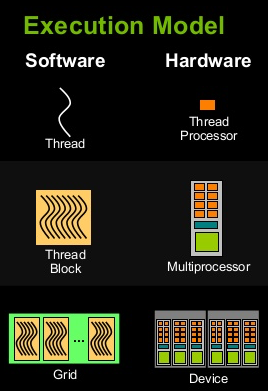
\includegraphics[width=\textwidth, height=0.8\textheight, keepaspectratio]{imgs/cuda}
      \end{figure}
    \end{column}
  \end{columns}

\end{frame}


\begin{frame}
  \frametitle{Intuition}

  \begin{itemize}
    \item GPUs have huge number of cores
    \item Use them to parallelize BFS
    \item One core per vertex, or one core per edge
    \item Vertex-based parallelism creates load imbalance for graphs with skewed degree distribution
    \item Edge-based parallelism requires high memory usage
  \end{itemize}
  \begin{itemize}
    \item Use vertex-based parallelism
    \item Virtualize high-degree vertices to address load imbalance
    \item Reduce memory usage by removing predecessors lists
  \end{itemize}

\end{frame}


\begin{frame}
  \frametitle{Difference}

  \begin{columns}[onlytextwidth]
    \begin{column}{0.5\textwidth}
      \begin{figure}[t]
        \centering
        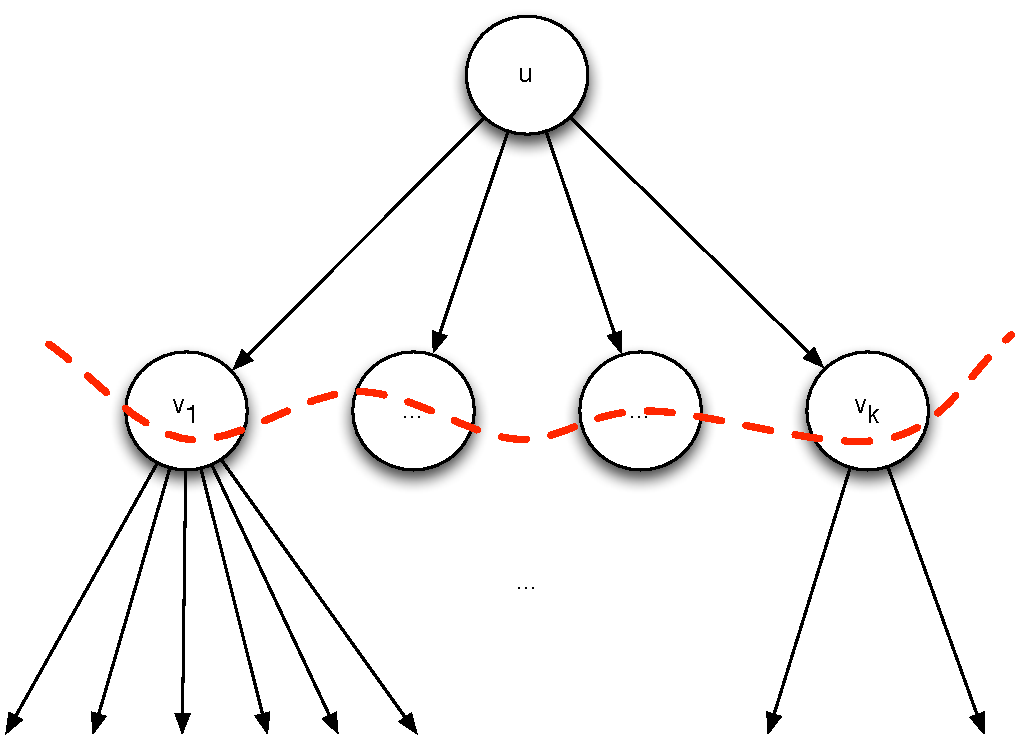
\includegraphics[width=\textwidth, height=0.6\textheight, keepaspectratio]{imgs/gpu-vertex-bfs}
        \caption{Vertex-based BFS}
      \end{figure}
    \end{column}

    \begin{column}{0.5\textwidth}
      \begin{figure}[t]
        \centering
        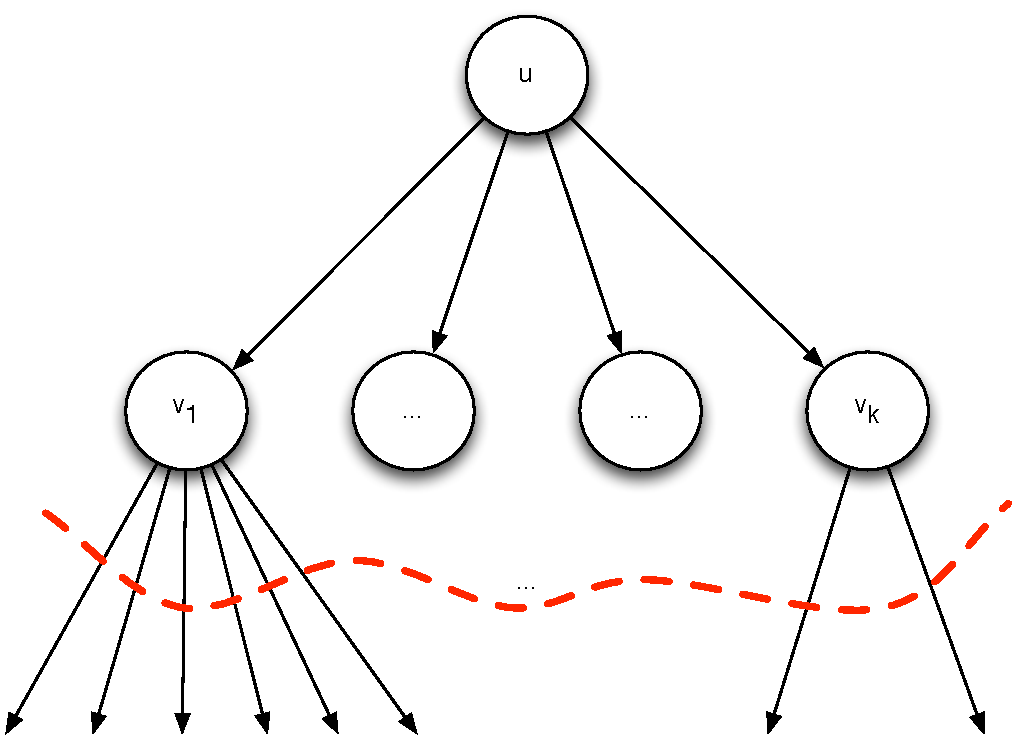
\includegraphics[width=\textwidth, height=0.6\textheight, keepaspectratio]{imgs/gpu-edge-bfs}
        \caption{Edge-based BFS}
      \end{figure}
    \end{column}
  \end{columns}

\end{frame}


\begin{frame}
  \frametitle{Vertex-based}

  \begin{columns}[onlytextwidth]
    \begin{column}{0.5\textwidth}
      \begin{itemize}
        \item For each level, for each vertex in parallel
        \item If vertex is on level
        \item For each neighbor, adjust \pred and \paths
        \item Atomic update on \paths needed (multiple paths can be discovered concurrently)
        \item While backtracking, if $u \in \pred(v)$ accumulate $\dep(u) = \dep(u) + \dep(v)$
        \item Possible load imbalance if degree skewed
      \end{itemize}
    \end{column}

    \begin{column}{0.5\textwidth}
      \begin{figure}[t]
        \centering
        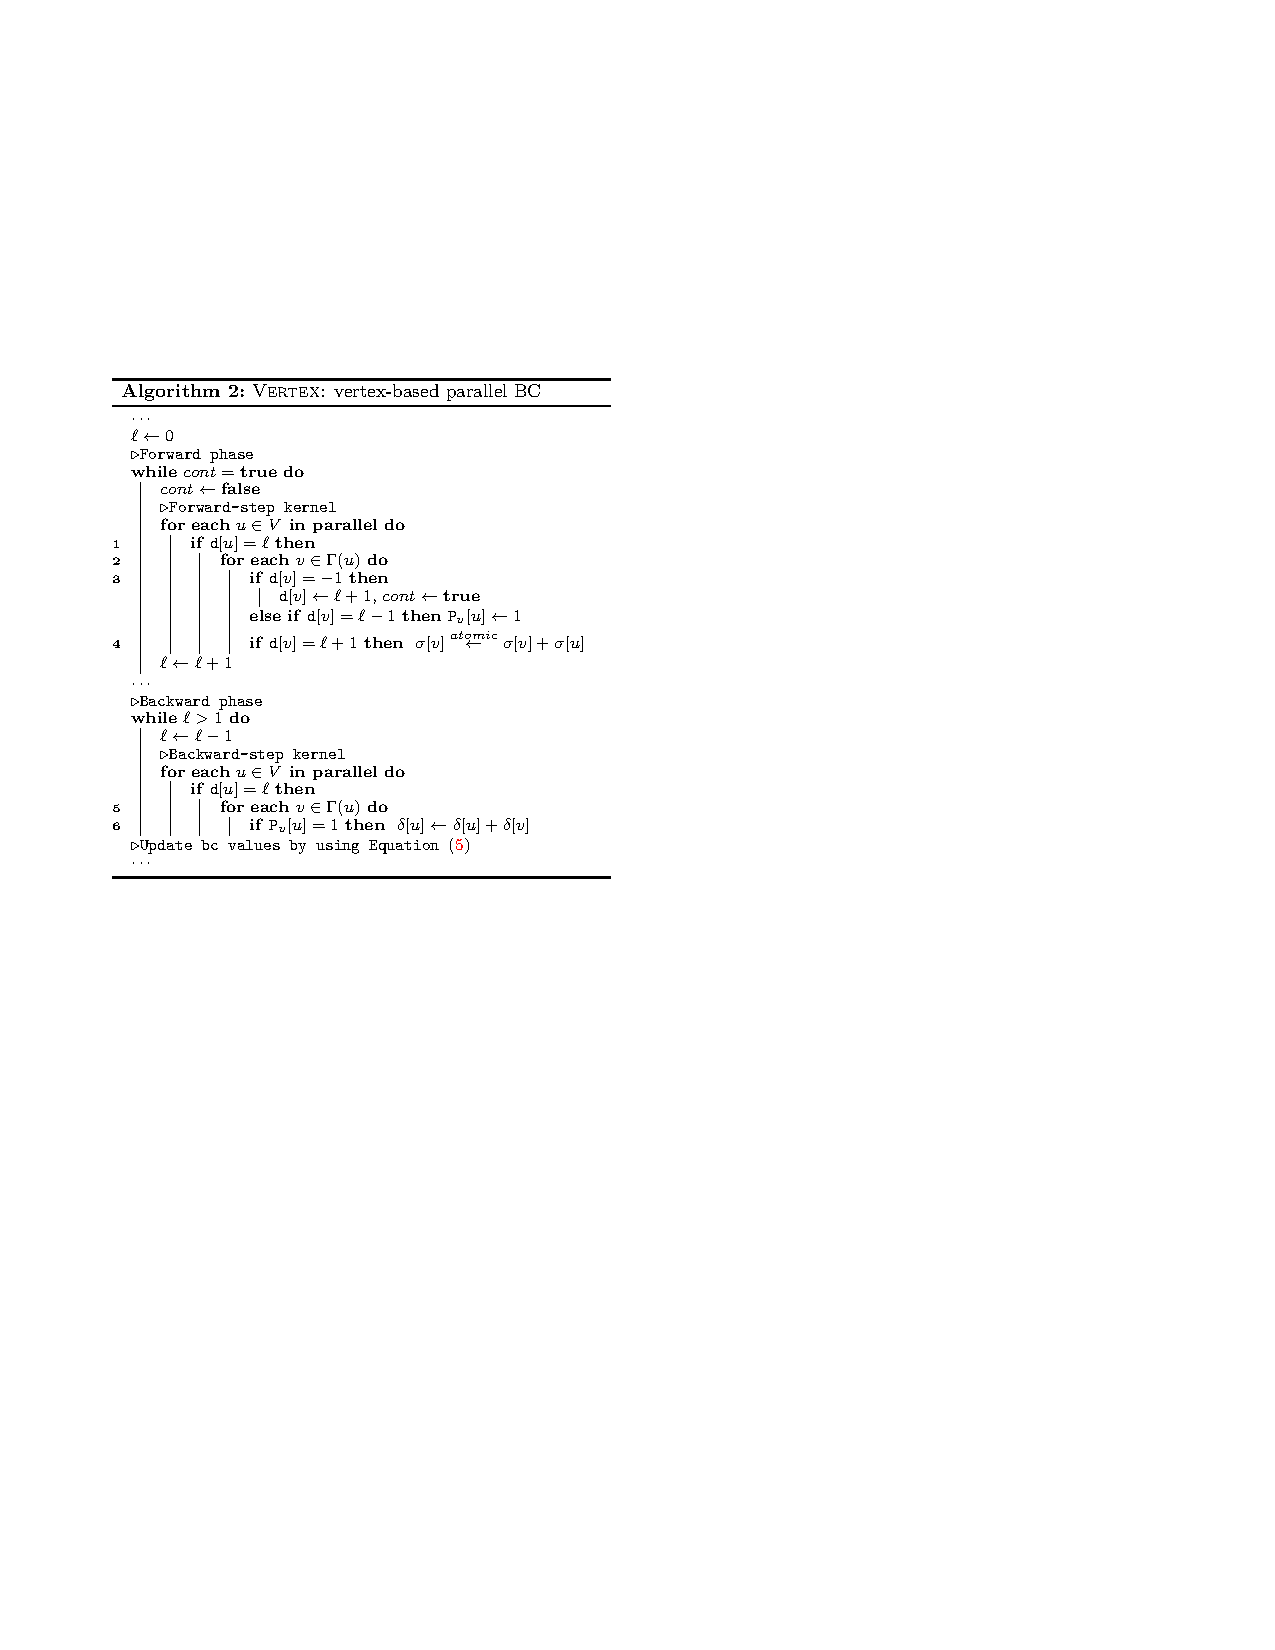
\includegraphics[width=\textwidth, height=0.8\textheight, keepaspectratio]{imgs/gpu-algo-vertex}
      \end{figure}
    \end{column}
  \end{columns}

\end{frame}


\begin{frame}
  \frametitle{Edge-based}

  \begin{columns}[onlytextwidth]
    \begin{column}{0.5\textwidth}
      \begin{itemize}
        \item For each level, for each edge in parallel
        \item If edge endpoint is on level
        \item Same as above...
        \item While backtracking, if $u \in \pred(v)$ accumulate $\dep(u) = \dep(u) + \dep(v)$ \emph{atomically}
        \item Multiple edges can try to update \dep concurrently
        \item More memory (edge-based layout) \\ and more atomic operations
      \end{itemize}
    \end{column}

    \begin{column}{0.5\textwidth}
      \begin{figure}[t]
        \centering
        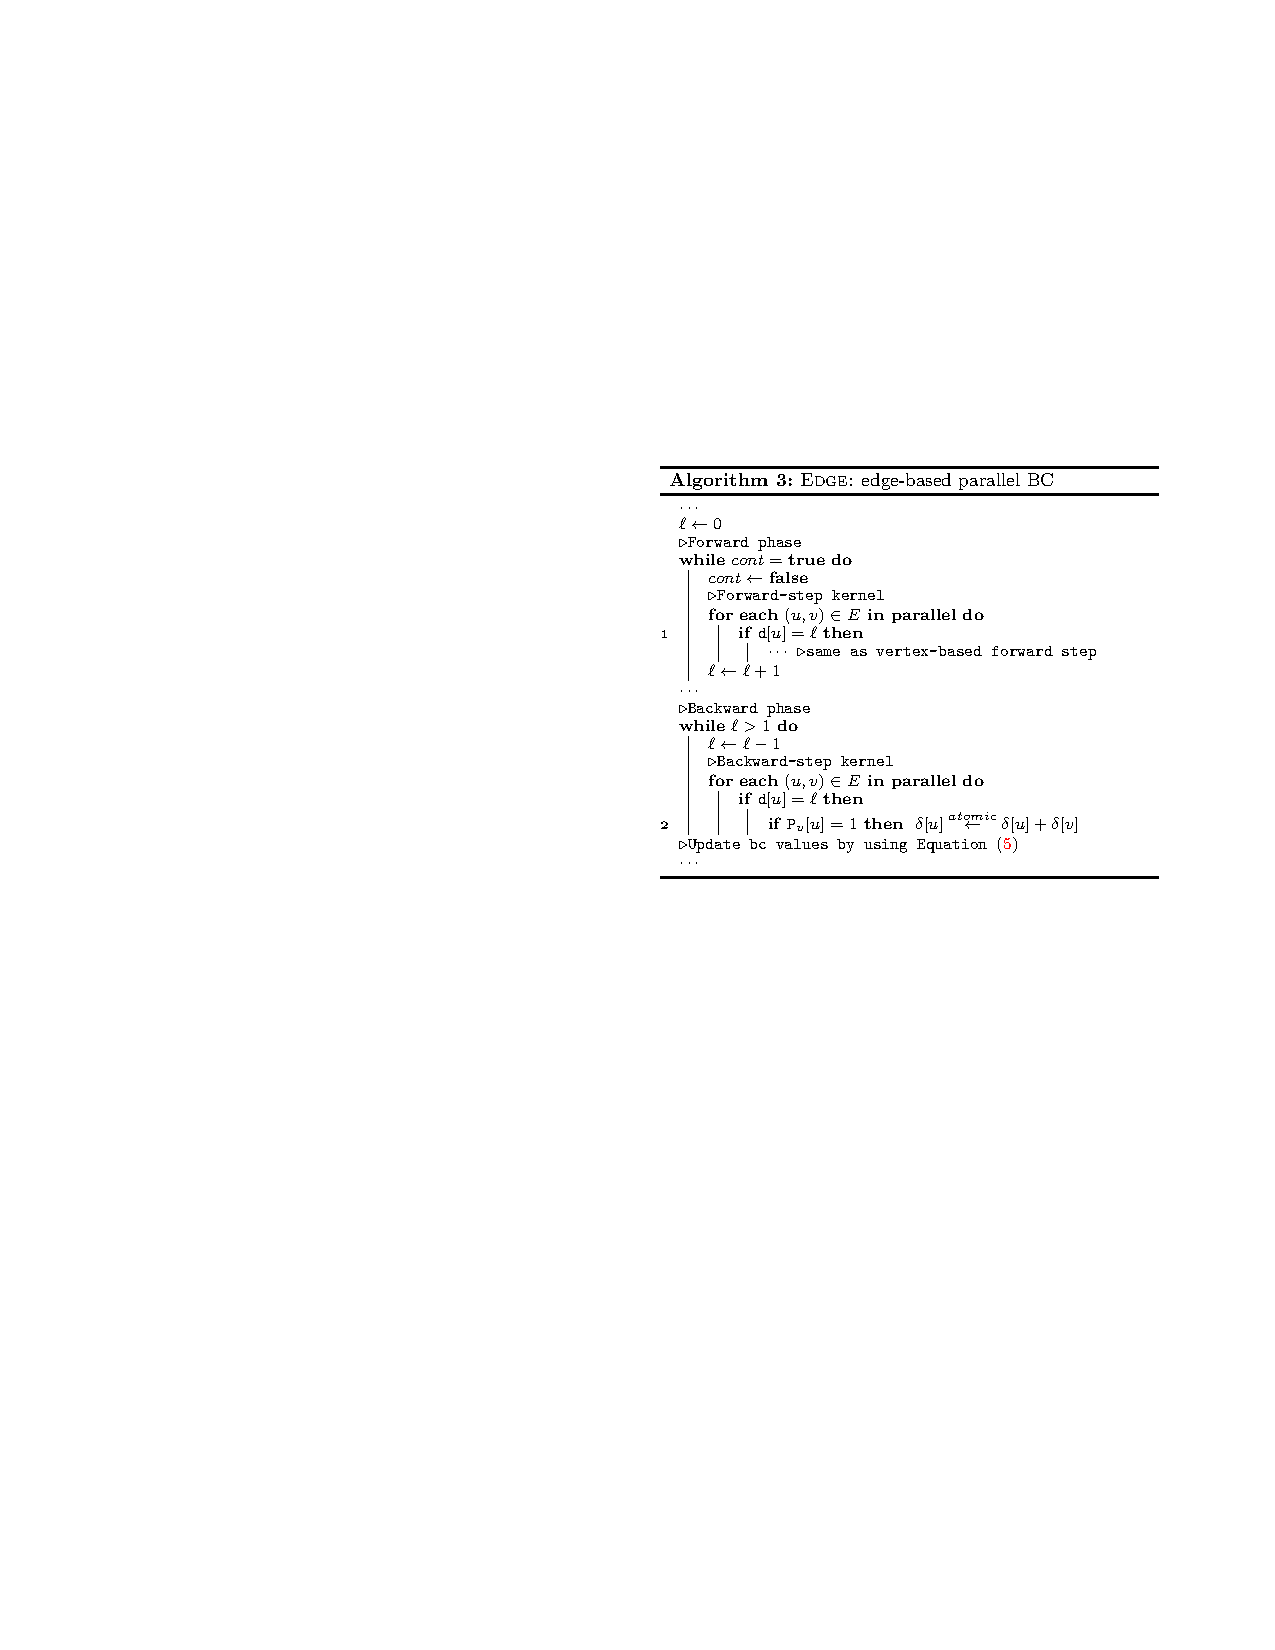
\includegraphics[width=\textwidth, height=0.8\textheight, keepaspectratio]{imgs/gpu-algo-edge}
      \end{figure}
    \end{column}
  \end{columns}

\end{frame}


\begin{frame}
  \frametitle{Vertex virtualization}

  \begin{columns}[onlytextwidth]
    \begin{column}{0.5\textwidth}
      \begin{itemize}
        \item AKA, edge packing/batching, \\ hybrid between vertex- and edge-based
        \item Split high degree vertices into virtual ones with maximum degree $mdeg$
        \item Equivalently, pack up to $mdeg$ edges belonging to the same vertex together
        \item Very small $mdeg = 4$
        \item Need additional auxiliary maps
      \end{itemize}
    \end{column}

    \begin{column}{0.5\textwidth}
      \begin{figure}[t]
        \centering
        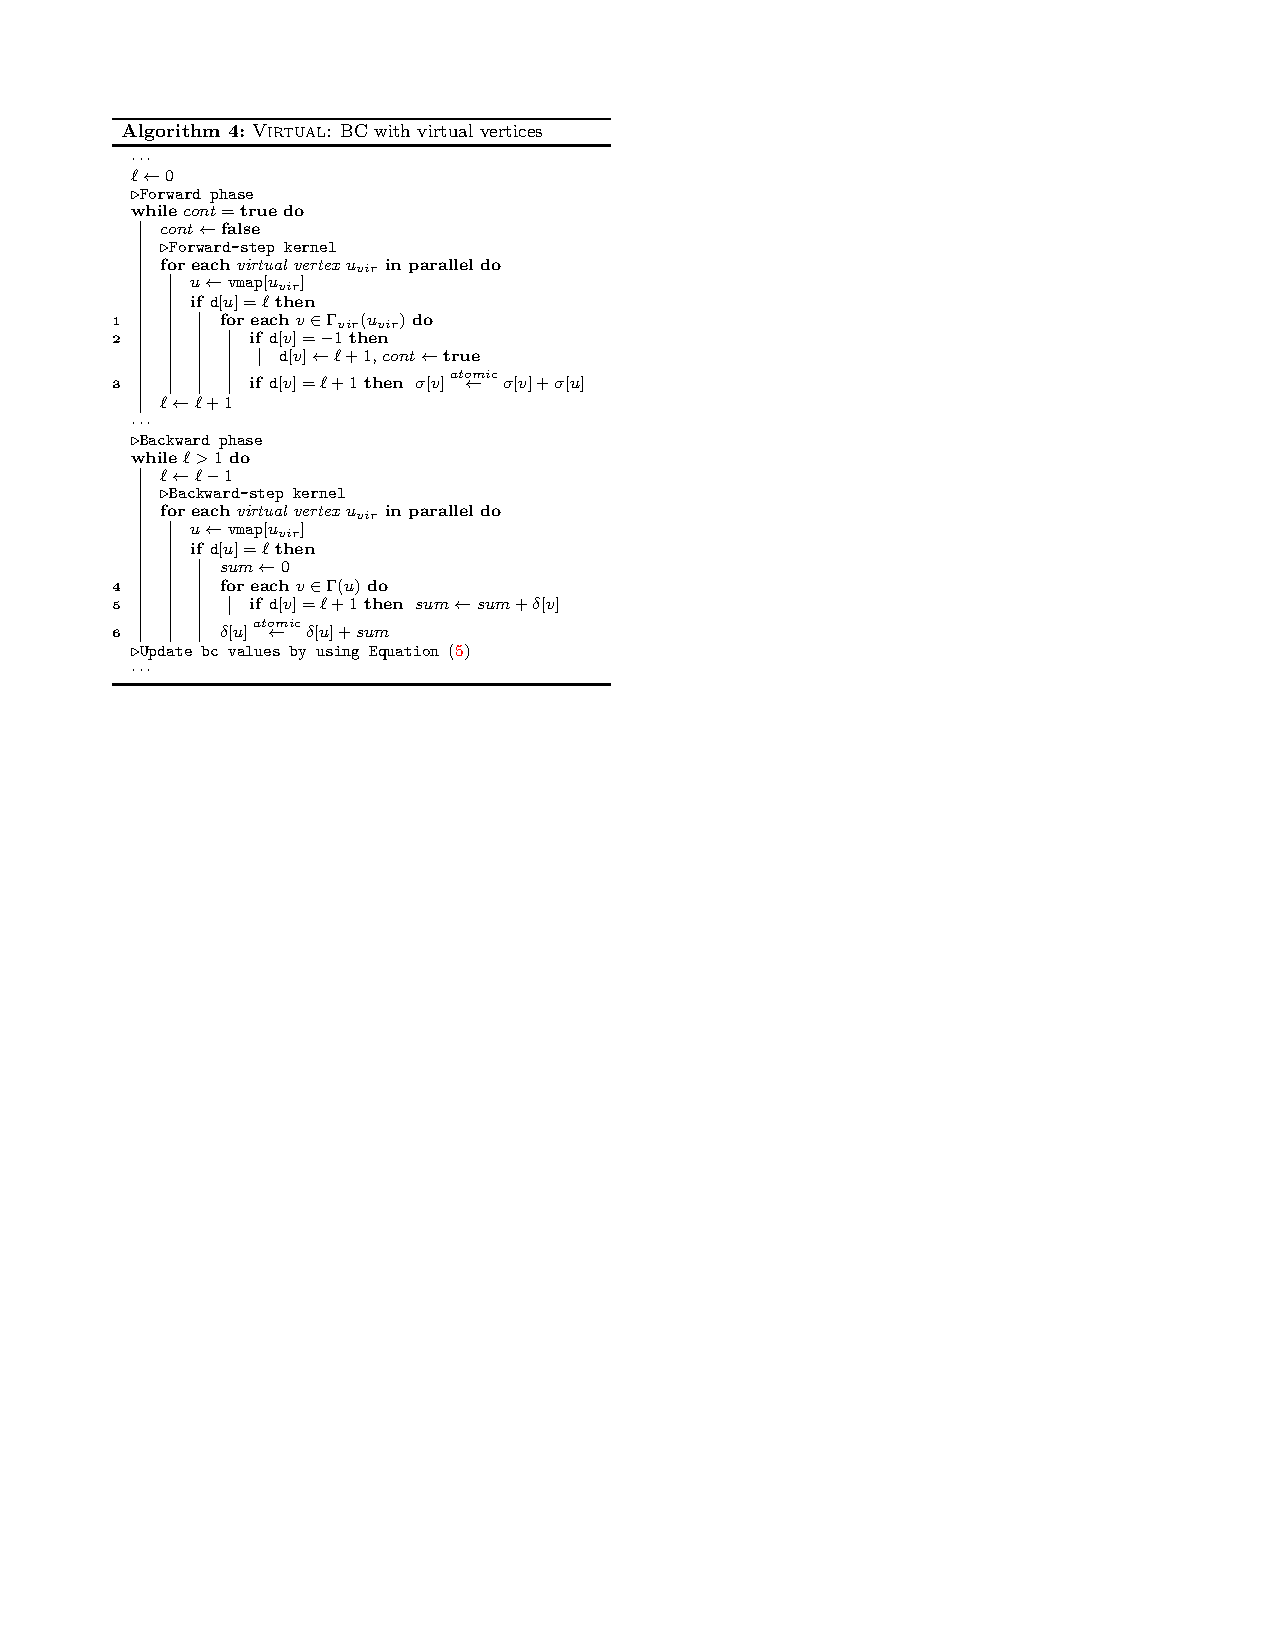
\includegraphics[width=\textwidth, height=0.8\textheight, keepaspectratio]{imgs/gpu-algo-hybrid}
      \end{figure}
    \end{column}
  \end{columns}

\end{frame}


\begin{frame}
  \frametitle{Benefits}

  \begin{itemize}
    \item Compared to vertex-based:
      \begin{itemize}
        \item Reduce load imbalance
      \end{itemize}
    \item Compared to edge-based:
      \begin{itemize}
        \item Reduce number of atomic operations
        \item Reduce memory footprint
      \end{itemize}
    \item Predecessors stored implicitly in the \spdag level (reduced memory usage)
    \item Memory layout can be further optimized to coalesce latency via \emph{striding}:
      \begin{itemize}
        \item Distribute edges to virtual vertices in round-robin
        \item When accessed in parallel, they create faster sequential memory access pattern
      \end{itemize}
  \end{itemize}
\end{frame}


\begin{frame}
  \frametitle{Results}

  \begin{figure}[t]
    \centering
    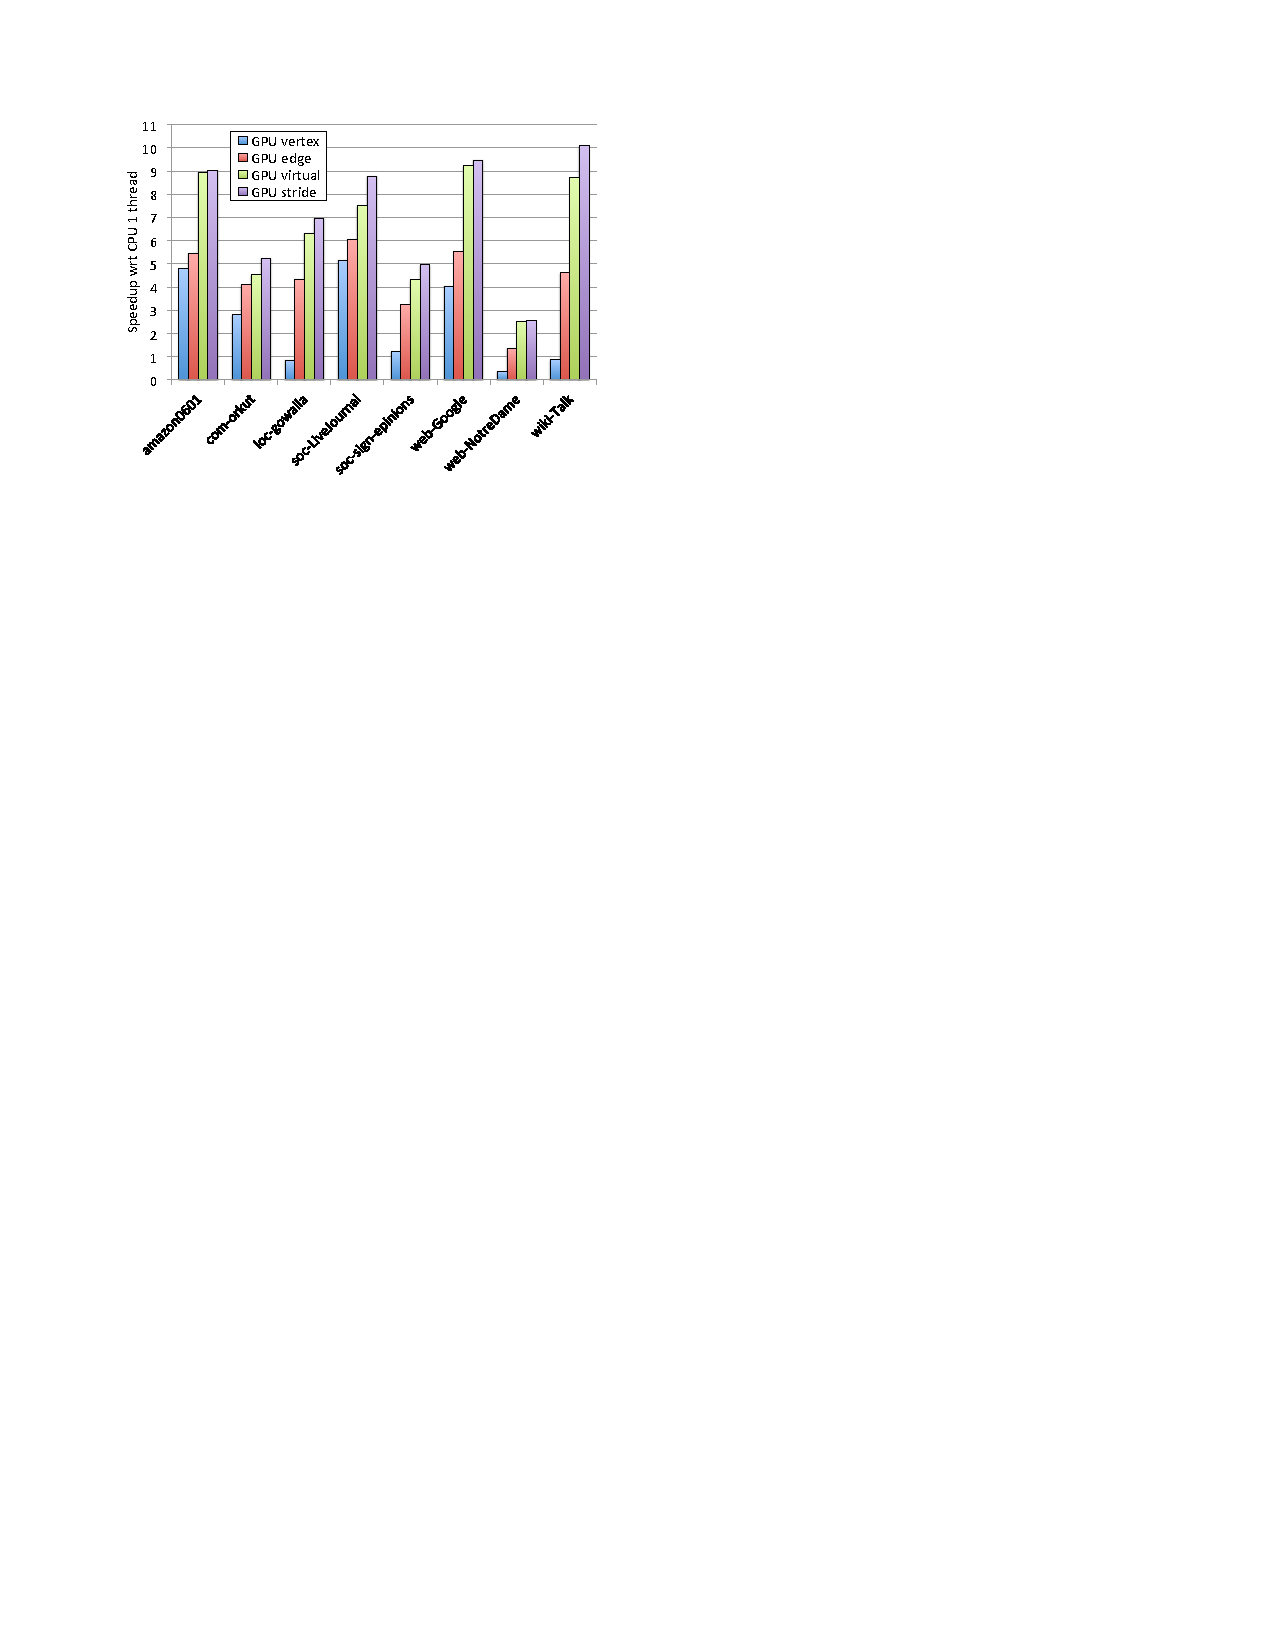
\includegraphics[width=\textwidth, height=0.6\textheight, keepaspectratio]{imgs/gpu-results1}
    \caption{Speedup over Brandes' on CPU on real graphs with 32-core GPU ($s= 1k, \ldots, 100k$)}
  \end{figure}

  \begin{itemize}
    \item Results computed only on a sample of sources and extrapolated linearly
  \end{itemize}
\end{frame}


%\begin{frame}
%  \frametitle{Results}
%
%  \begin{figure}[t]
%    \centering
%    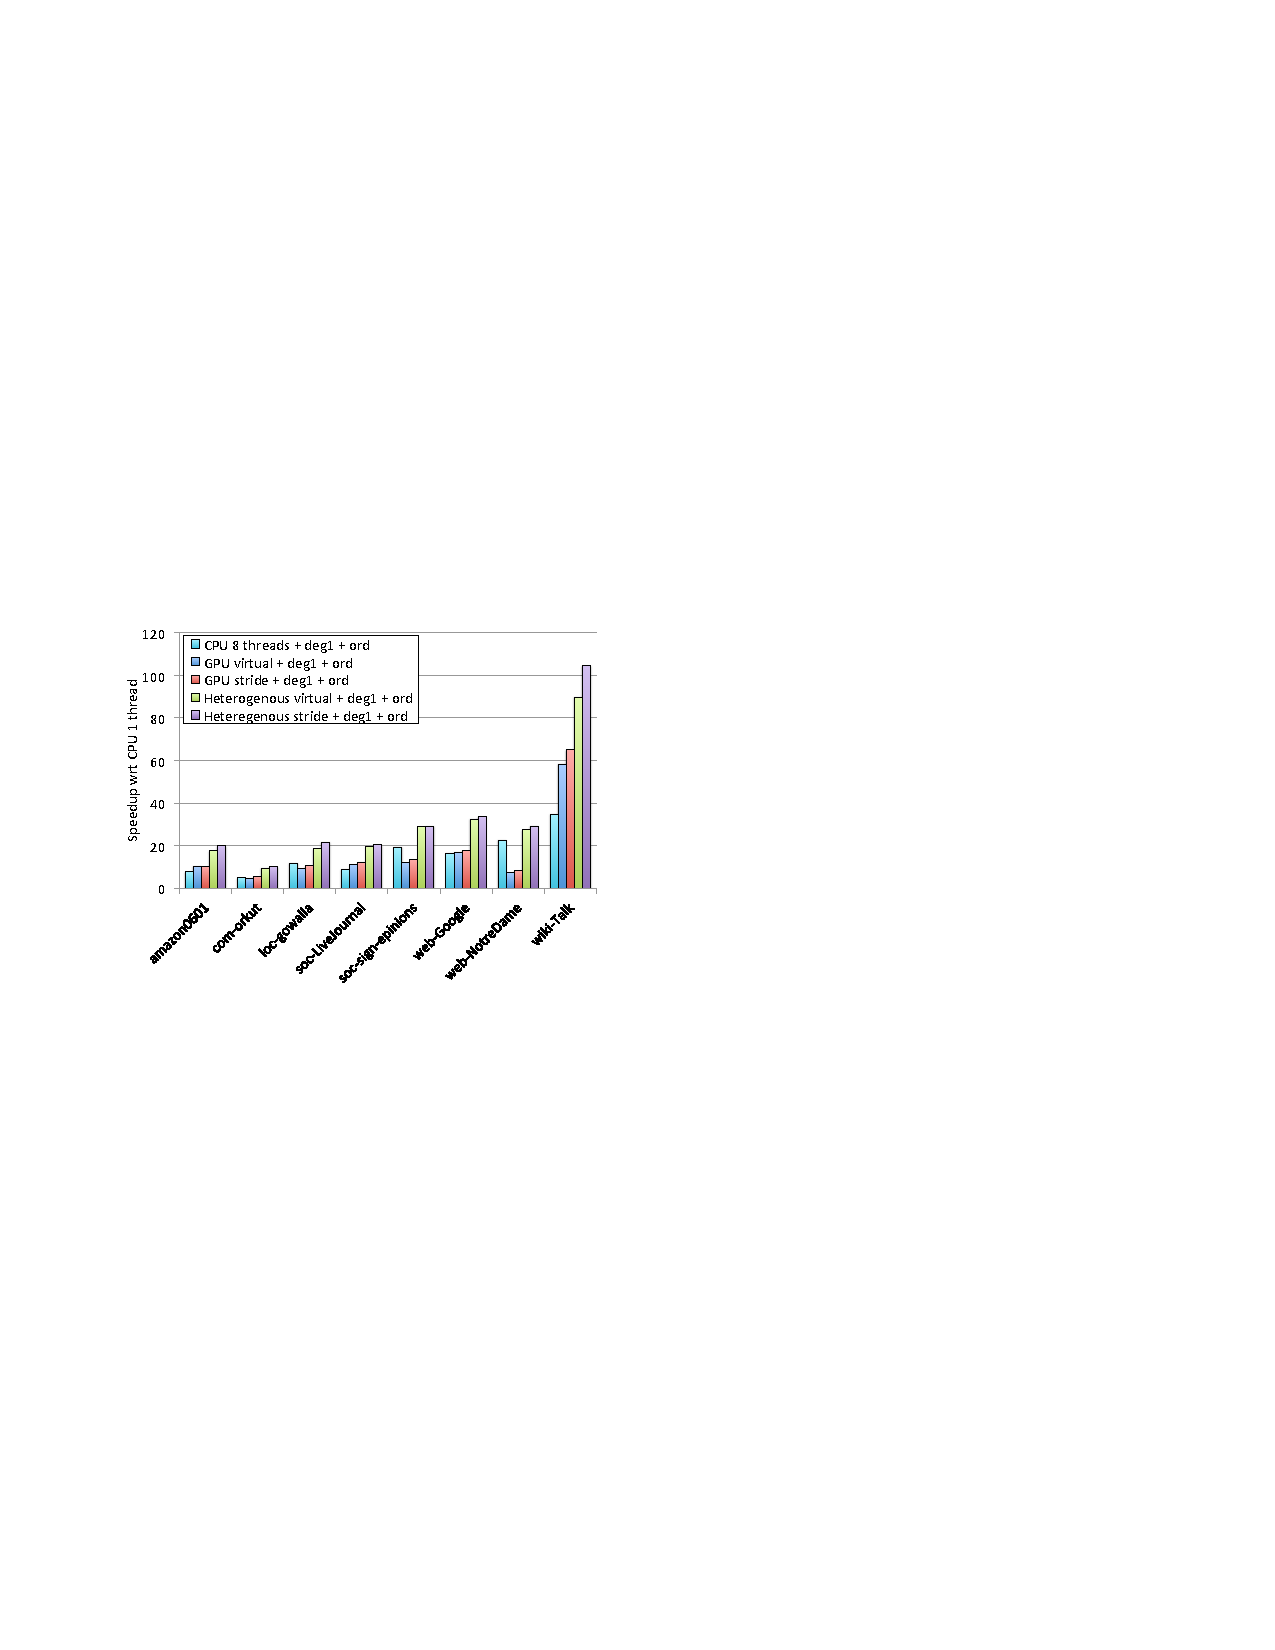
\includegraphics[width=\textwidth, height=0.6\textheight, keepaspectratio]{imgs/gpu-results2}
%    \caption{Speedup over Brandes' on CPU on real graphs with 32-core GPU}
%  \end{figure}
%
%\end{frame}



\subsection{Exact Algorithms for Dynamic Graphs}

%% Green et al.
\begin{frame}
  \centering
  \vfill
  {\huge A Fast Algorithm for Streaming Betweenness Centrality}
  \vfill
  {\Large O. Green, R. McColl, D. A. Bader}
  \vfill
  {\large SocialCom '12: International Conference on Social Computing}
  \vfill
\end{frame}


\begin{frame}
  \frametitle{Intuition}

  \begin{itemize}
    \item Make Brandes' algorithm incremental
    \item Keep additional data structures to avoid recomputing partial results
      \begin{itemize}
        \item Rooted \spdag for each source $s \in V$
        \item Depth in the tree for $t$ = distance of $t$ from $s$
      \end{itemize}
    \item Re-run parts of modified Brandes' algorithm on edge update
    \item Support only edge addition (on unweighted graphs)
  \end{itemize}

\end{frame}


\begin{frame}
  \frametitle{Data structures}

  \begin{itemize}
    \item One $\spdag_s$ for each source $s \in V$, which contains for each other vertex $t \in V$:
      \begin{itemize}
        \item Distance $\dist_{st}$, paths $\paths_{st}$, dependencies $\dep_{s}(t)$, predecessors $\pred_{s}(t)$
        \item Additional per-level queues for exploration
      \end{itemize}
  \end{itemize}
  \begin{itemize}
    \item On addition of edge $(u,v)$, let $dd = |d_{su} - d_{sv}|$:
      \begin{itemize}
        \item $dd = 0$ same~level
        \item $dd = 1$ adjacent~level
        \item $dd > 1$ non-adjacent~level
      \end{itemize}
  \end{itemize}

\end{frame}


\begin{frame}
  \frametitle{Same level addition}
  \begin{columns}[onlytextwidth]

    \begin{column}{0.5\textwidth}
      \begin{itemize}
        \item $dd = 0$
        \item Edge creates no new shortest paths
        \item No change to betweenness \\ due to this source
      \end{itemize}
    \end{column}

    \begin{column}{0.5\textwidth}
      \begin{figure}[t]
        \centering
        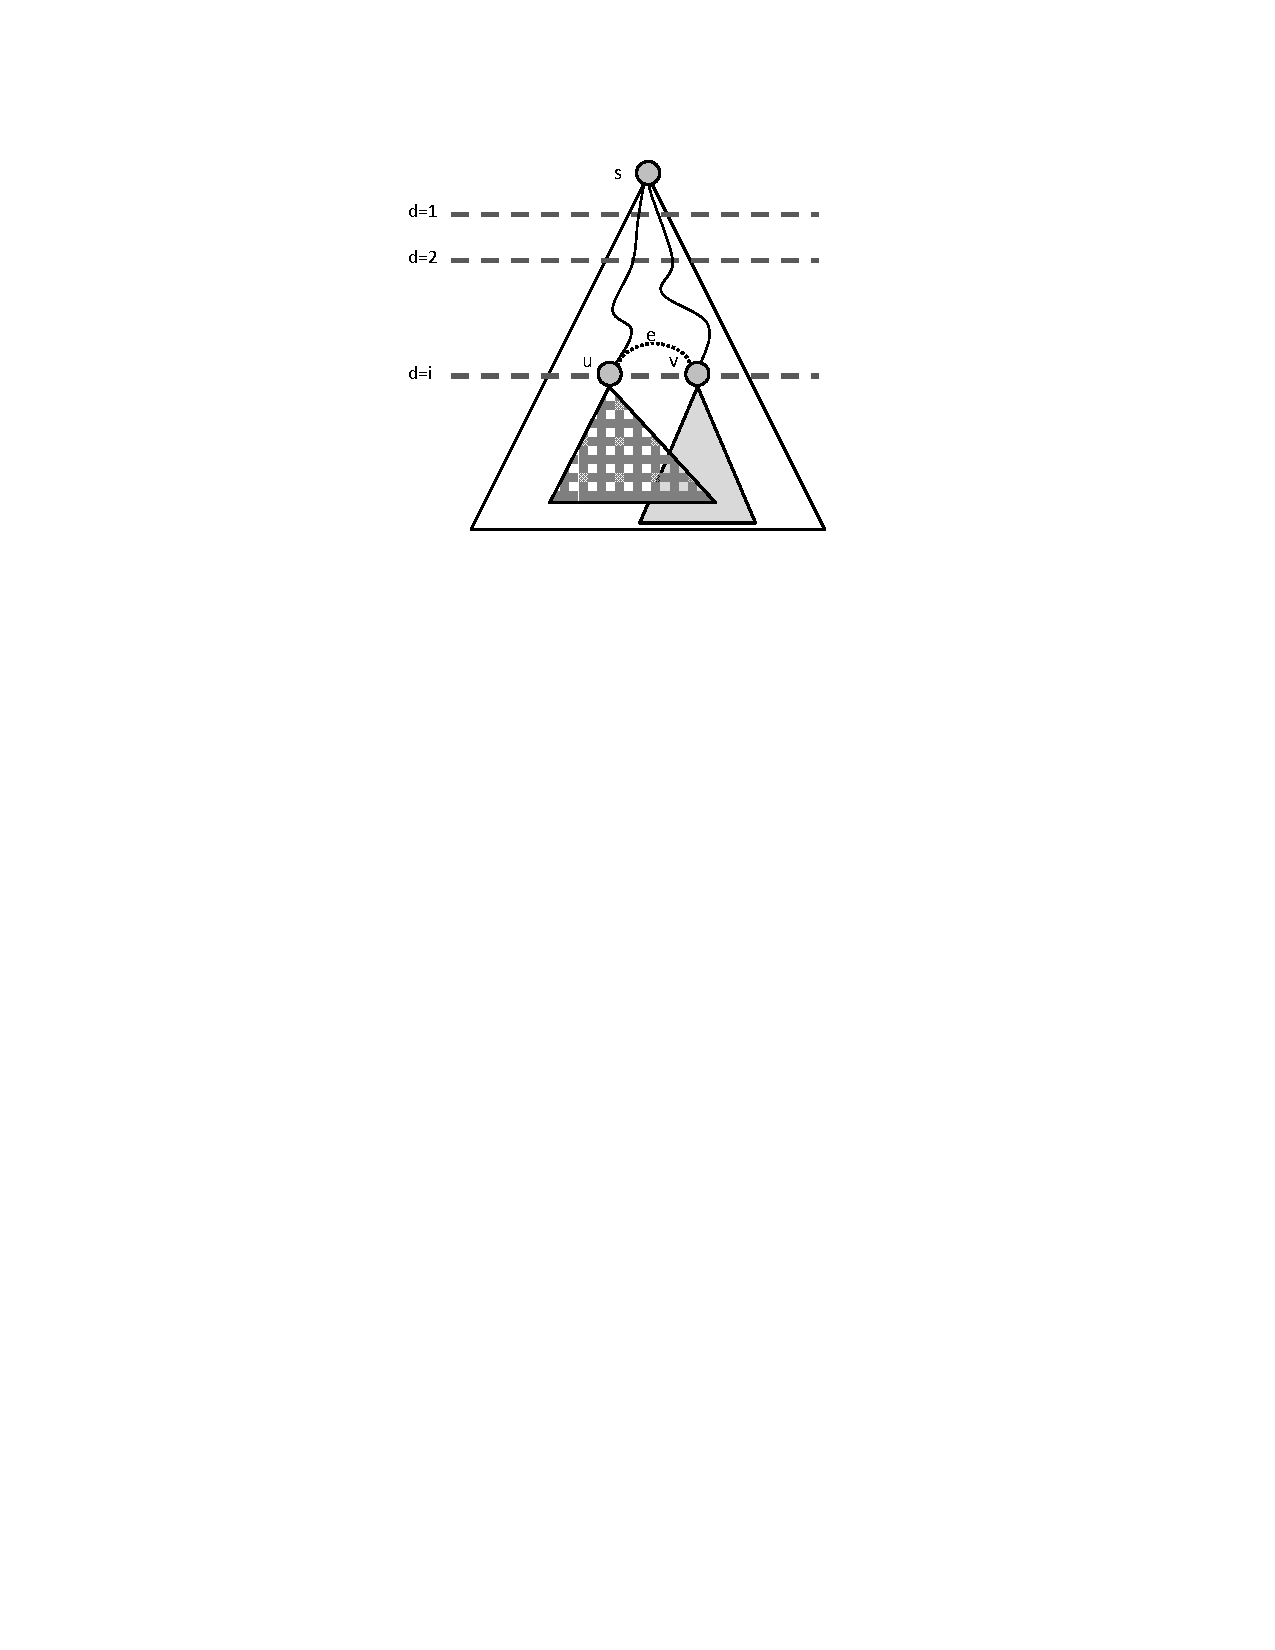
\includegraphics[width=\textwidth, height=\textheight, keepaspectratio]{imgs/green-0lvl-compressed}
      \end{figure}
    \end{column}
  \end{columns}

\end{frame}


\begin{frame}
  \frametitle{Adjacent level addition}
  \begin{columns}[onlytextwidth]

    \begin{column}{0.5\textwidth}
      \begin{itemize}
        \item $dd = 1$
        \item Let $u_{high} = u ,\, u_{low} = v$
        \item Edge creates new shortest paths
        \item \spdag unchanged
        \item Changes in \paths confined to sub-dag rooted in $u_{low}$
        \item Changes in \dep also spread above to decrease old dependency and account for new dependency
        \item Example: $w$ and predecessors have now only $\sfrac{1}{2}$ of dependency on sub-dag rooted in $u_{low}$
      \end{itemize}
    \end{column}

    \begin{column}{0.5\textwidth}
      \begin{figure}[t]
        \centering
        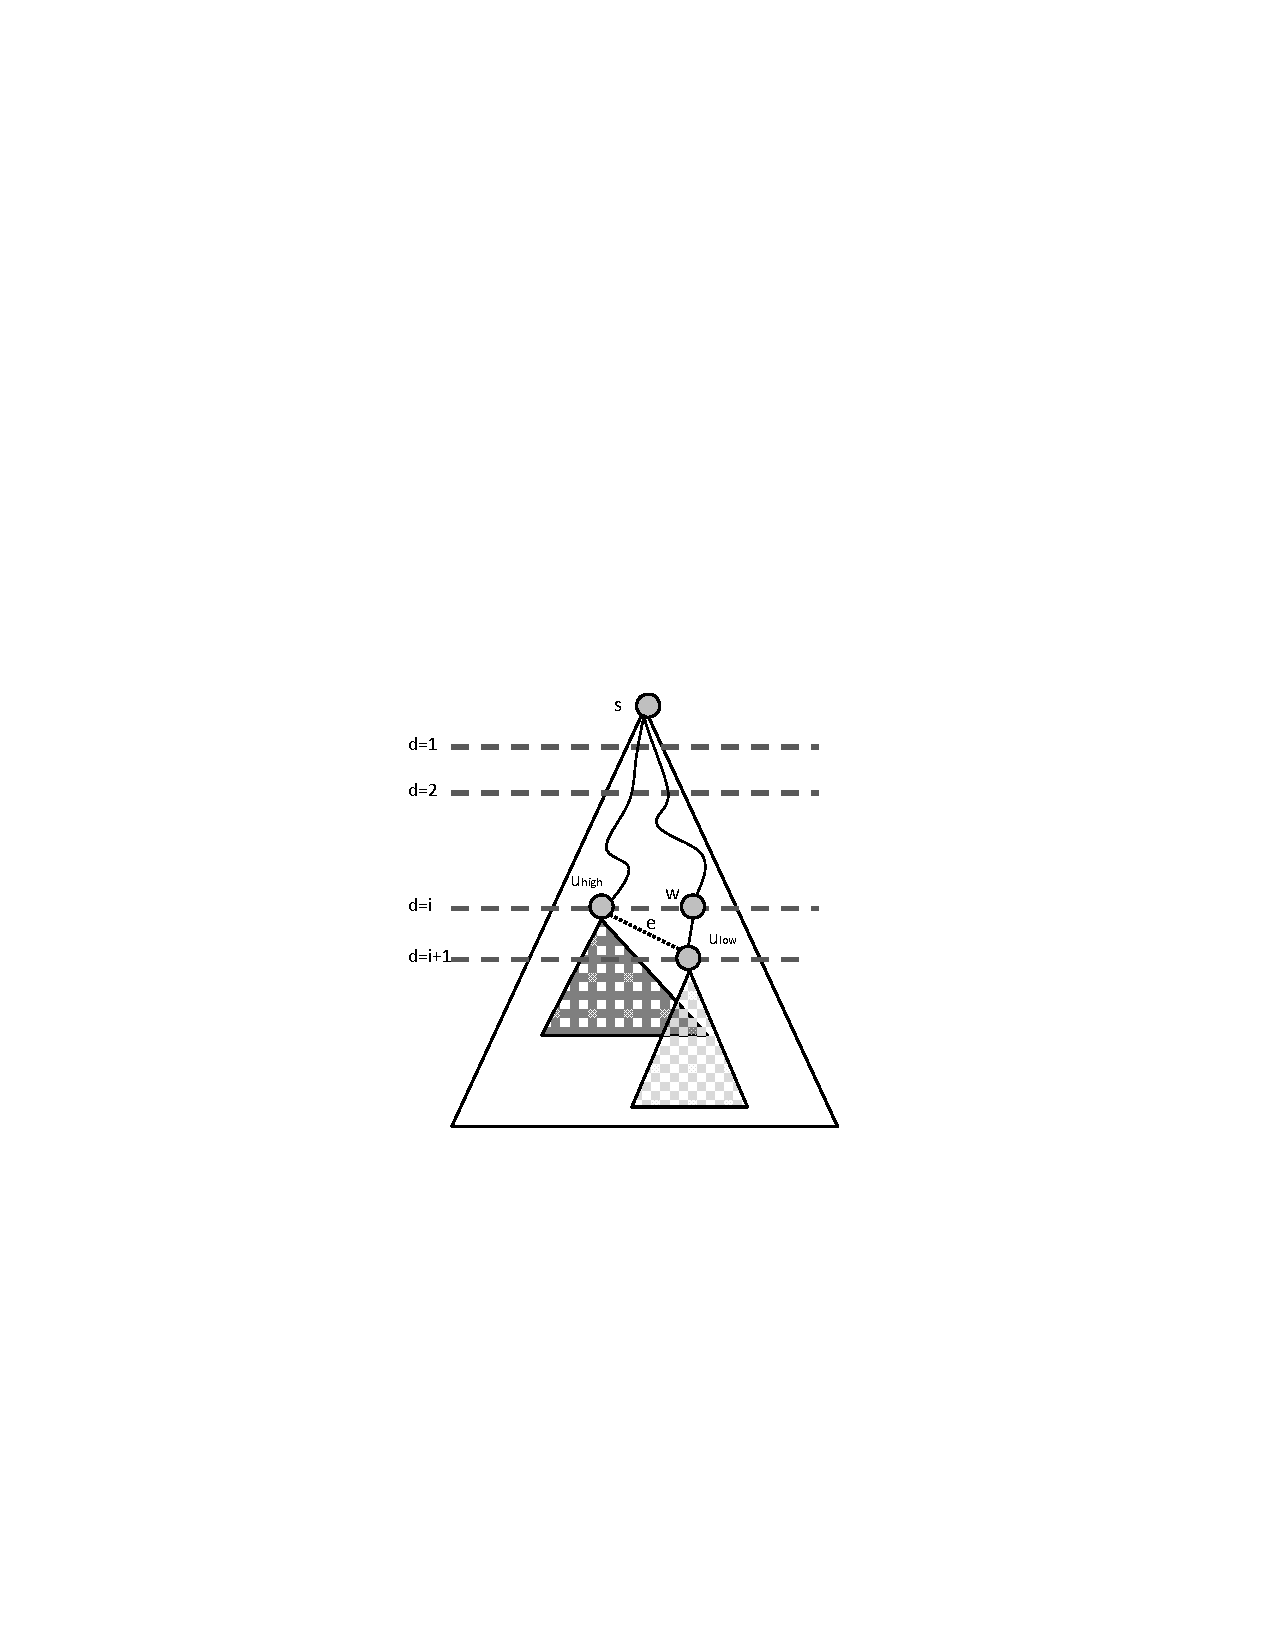
\includegraphics[width=\textwidth, height=\textheight, keepaspectratio]{imgs/green-1lvl-compressed}
      \end{figure}
    \end{column}
  \end{columns}

\end{frame}


\begin{frame}
  \frametitle{Algorithm}
  \begin{columns}[onlytextwidth]

    \begin{column}{0.3\textwidth}
      \begin{itemize}
        \item During exploration:
          \begin{itemize}
            \item Fix \paths
            \item Mark visited vertices
            \item Enqueue for further processing
          \end{itemize}
      \end{itemize}
      \begin{itemize}
        \item During backtracking:%
          \begin{itemize}
            \item Fix \dep and \betw
            \item Recurse up the whole \spdag
          \end{itemize}
      \end{itemize}
    \end{column}

    \begin{column}{0.7\textwidth}
      \begin{figure}[t]
        \centering
        %        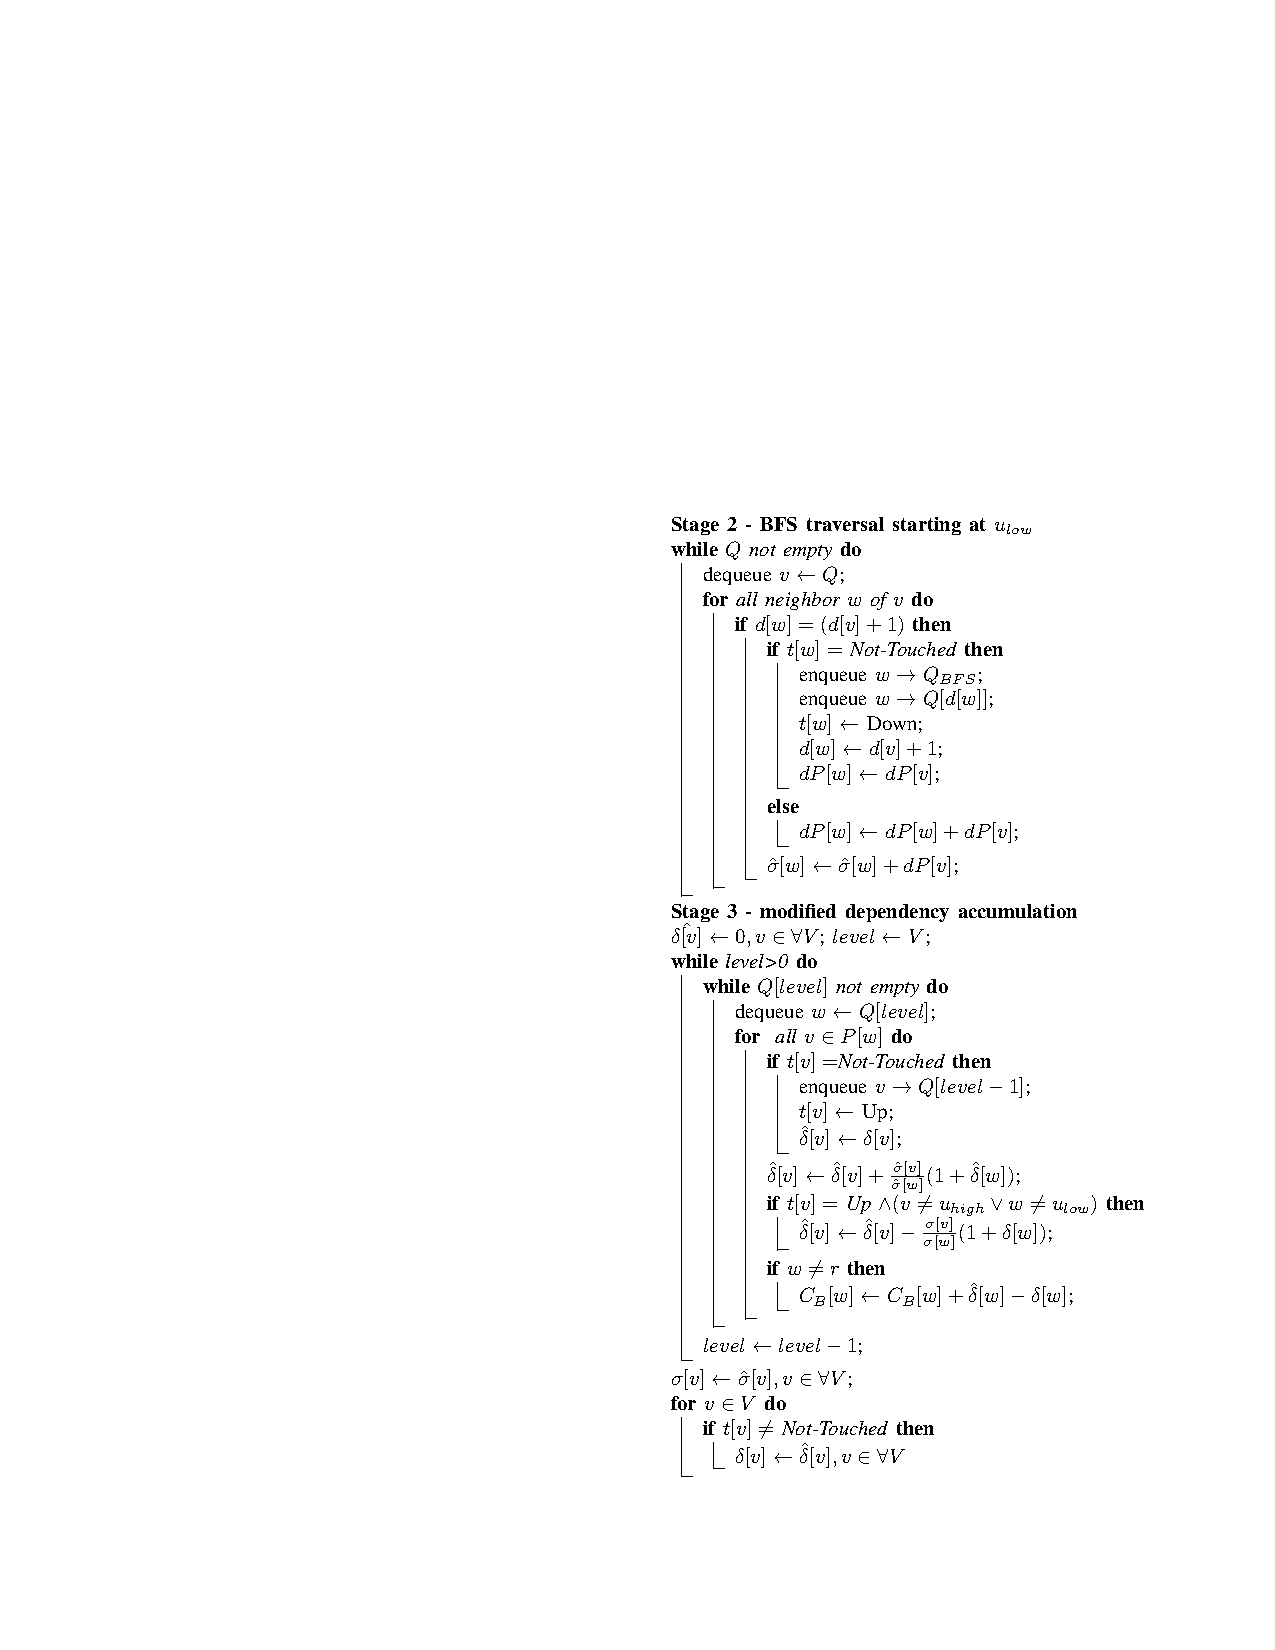
\includegraphics[width=\textwidth, height=0.8\textheight, keepaspectratio]{imgs/green-algo}
        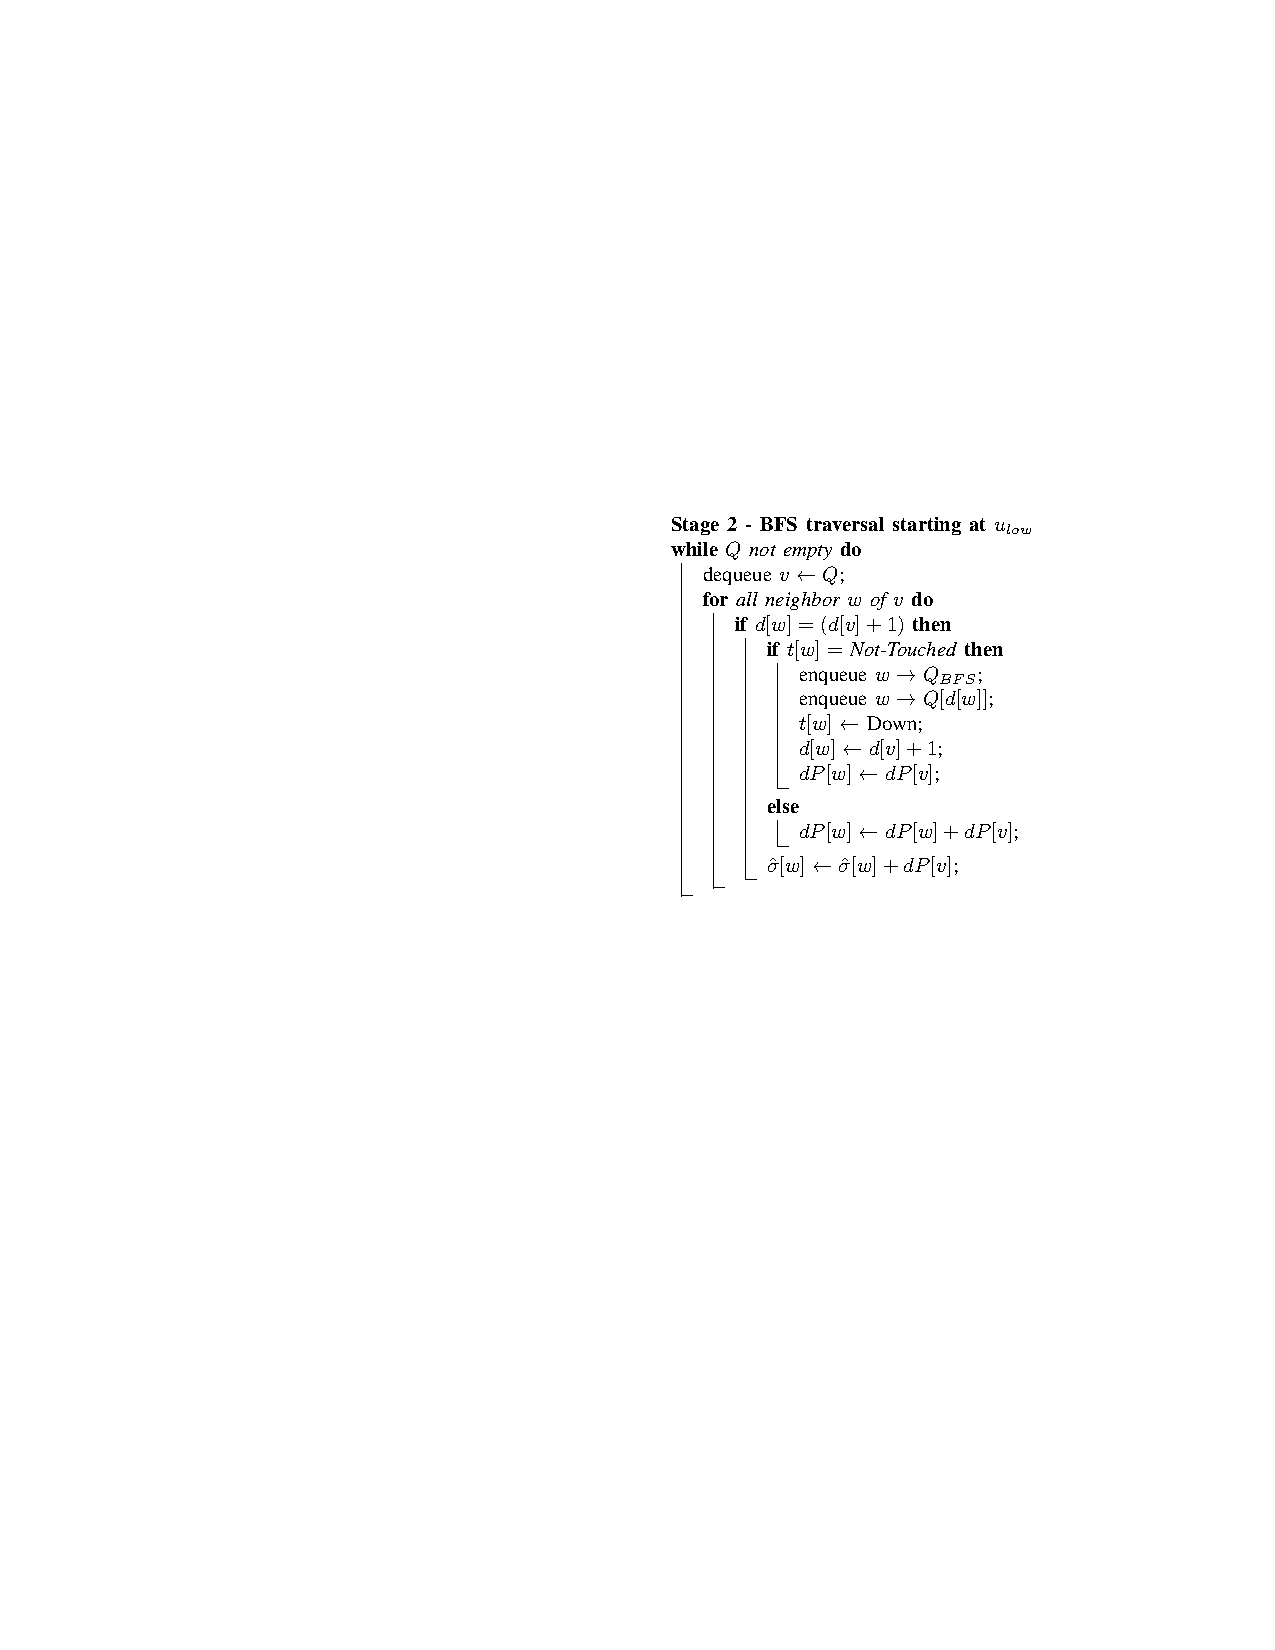
\includegraphics[width=0.45\textwidth, height=0.8\textheight, keepaspectratio, valign=t]{imgs/green-algo1}
        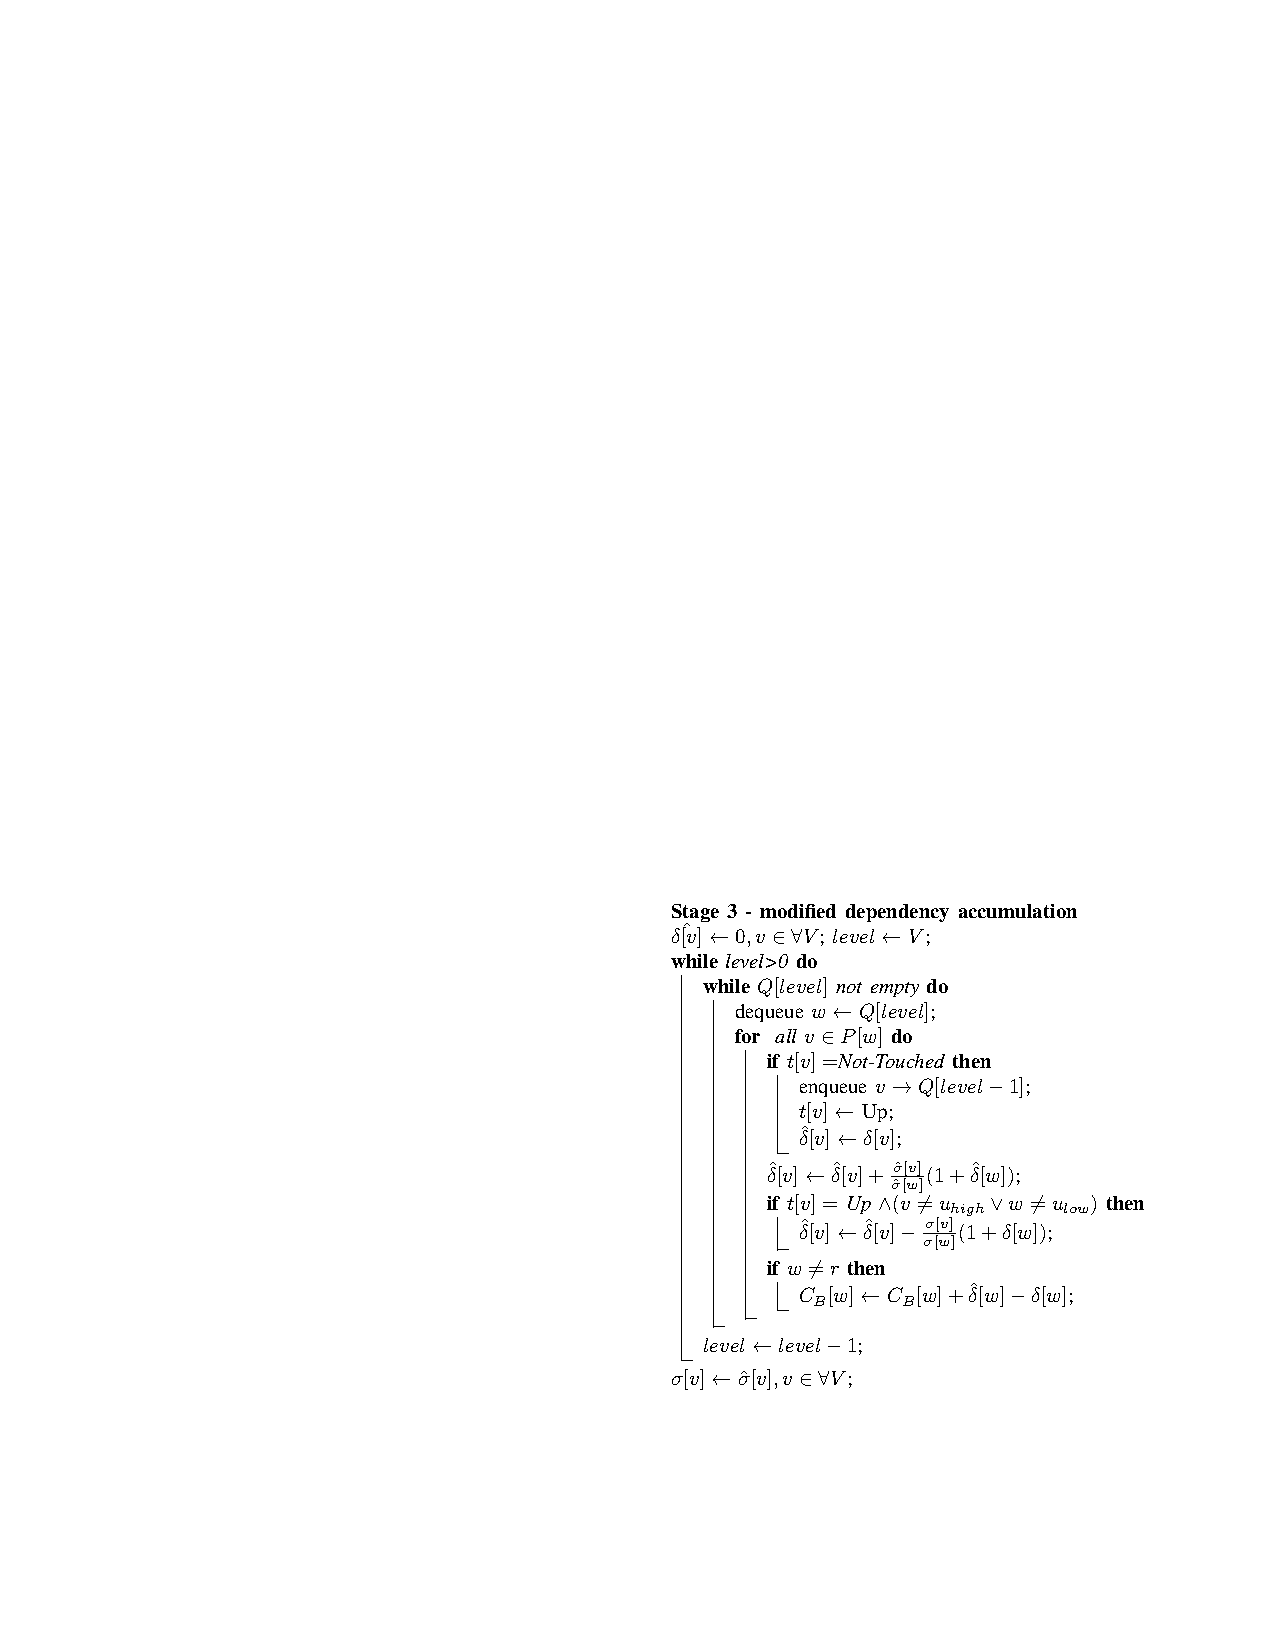
\includegraphics[width=0.6\textwidth, height=0.8\textheight, keepaspectratio, valign=t]{imgs/green-algo2}
      \end{figure}
    \end{column}
  \end{columns}
\end{frame}


\begin{frame}
  \frametitle{Non-adjacent level addition}

  \begin{columns}[onlytextwidth]

    \begin{column}{0.5\textwidth}
      \begin{itemize}
        \item $dd > 1$
        \item Edge creates new shortest paths
        \item Changes to \spdag (new distances)
        \item Algorithm only sketched \\ (most details missing)
      \end{itemize}
    \end{column}

    \begin{column}{0.5\textwidth}
      \begin{figure}[t]
        \centering
        \includegraphics<1>[width=\textwidth, height=0.8\textheight, keepaspectratio]{imgs/green-2lvl-before-compressed}
        \transdissolve<2>
        \transduration{2}
        \includegraphics<2>[width=\textwidth, height=0.8\textheight, keepaspectratio]{imgs/green-2lvl-after-compressed}
      \end{figure}
    \end{column}
  \end{columns}

\end{frame}


\begin{frame}
  \frametitle{Complexity}

  \begin{itemize}
    \item Time: $O(n^2 + nm)$ $\leftarrow$ same as Brandes'
    \item In practice, algorithm is much faster
  \end{itemize}
  \begin{itemize}
    \item Space: $O(n^2 + nm)$ $\leftarrow$ higher than Brandes'
    \item For each source, a \spdag of complexity $n + m$
  \end{itemize}

\end{frame}


\begin{frame}
  \frametitle{Results}

  \begin{figure}[t]
    \centering
    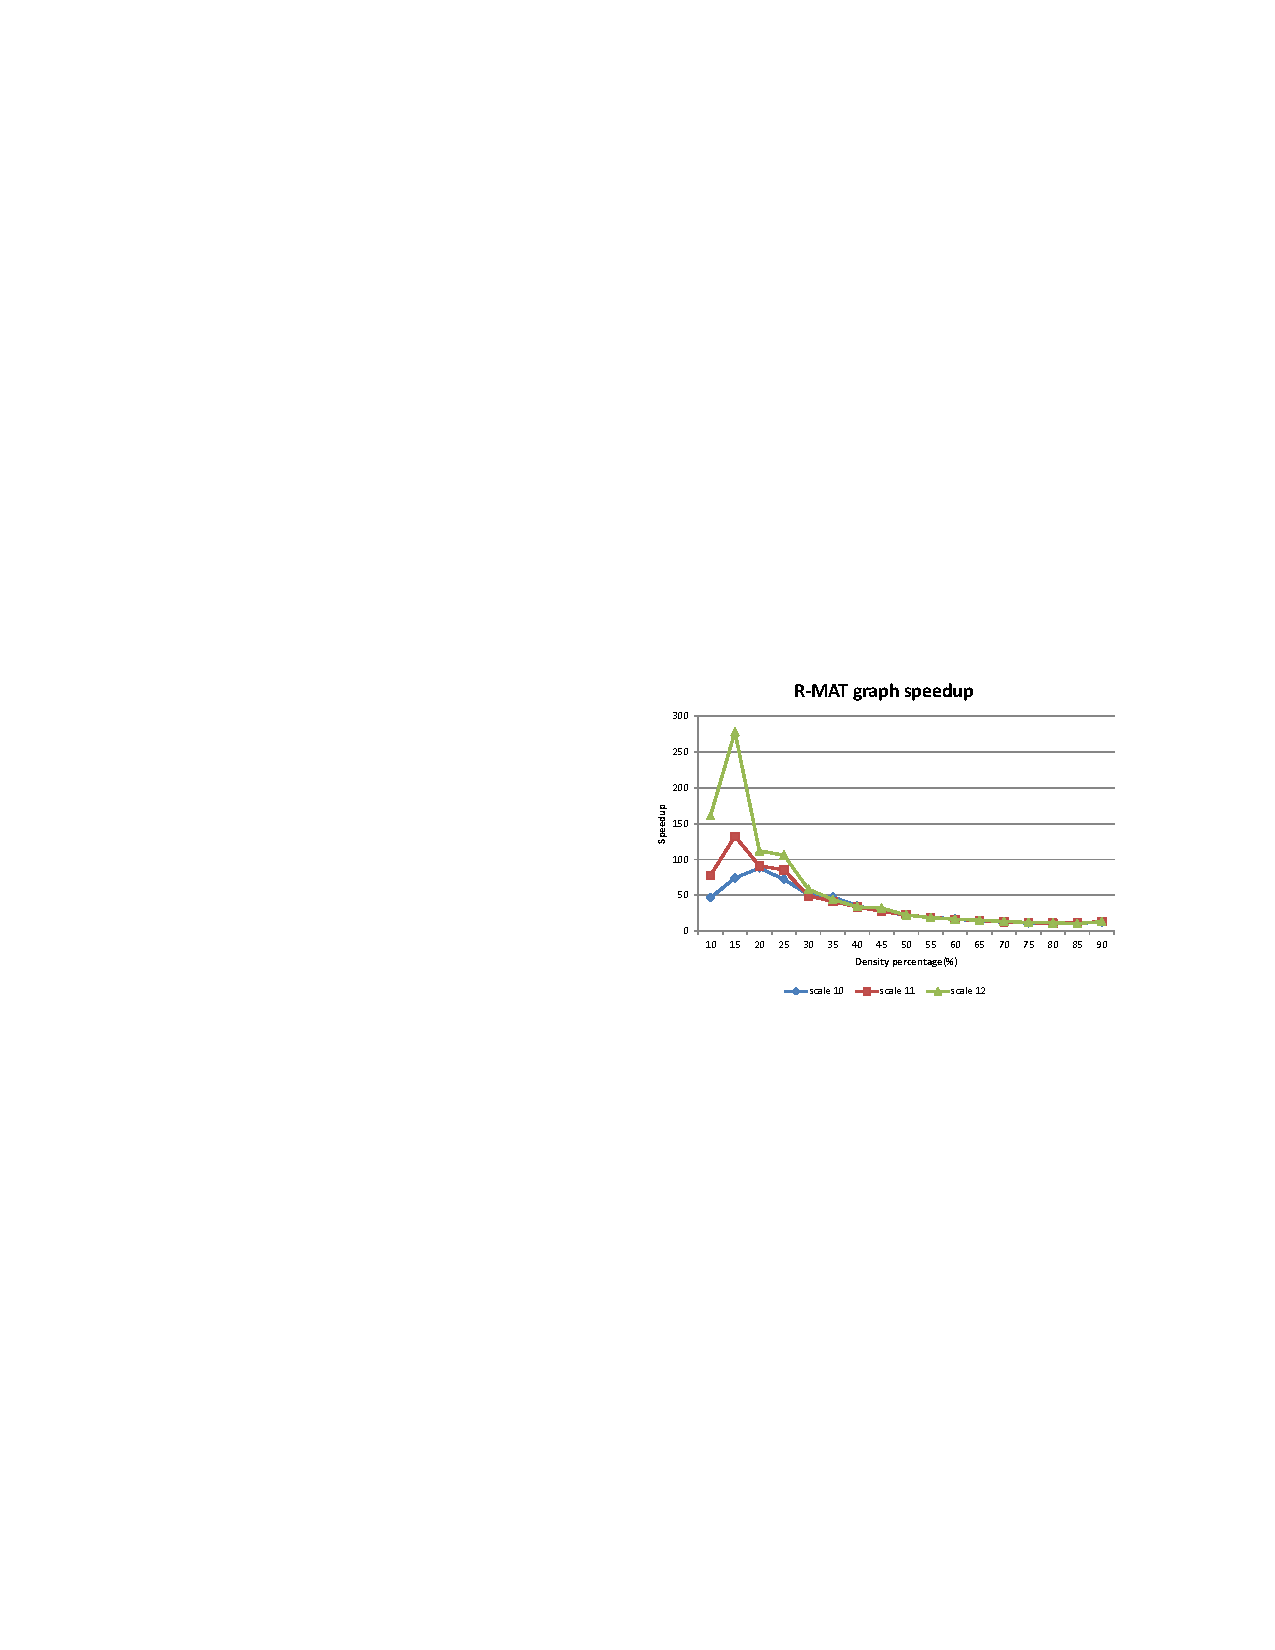
\includegraphics[width=\textwidth, height=0.7\textheight, keepaspectratio]{imgs/green-results1}
    \caption{Speedup over Brandes' on synthetic graphs ($n = 4096$)}
  \end{figure}

\end{frame}


\begin{frame}
  \frametitle{Conclusions}

  \begin{itemize}
    \item Up to 2 orders of magnitude speedup
    \item Super-quadratic space bottleneck
  \end{itemize}

\end{frame}


%% QUBE
\begin{frame}
  \centering
  \vfill
  {\huge QUBE: a Quick Algorithm for Updating Betweenness centrality}
  \vfill
  {\Large M. Lee, J. Lee, J. Park, R. Choi, C. Chung}
  \vfill
  {\large WWW '12: International World Wide Web Conference}
  \vfill
\end{frame}

\begin{frame}
  \frametitle{Intuition}

  \begin{itemize}
    \item No need to update all vertices when a new edge is added
    \item Prune vertices whose \betw does not change
    \item Large reduction in all-pairs shortest paths to be re-computed
    \item Support both edge additions and removals
  \end{itemize}
\end{frame}


\begin{frame}
  \frametitle{Minimum Cycle Basis}

  \begin{itemize}
    \item $G=(V,E)$ undirected graph
    \item \emph{Cycle} $C \subseteq E$ s.t. $\forall v \in V$, $v$ incident to even number of edges in $C$
    \item Represented as edge incidence vector $\nu \in \{ 0,1 \}^{|E|}$, where $\nu(e) = 1 \iff e \in C$
    \item \emph{Cycle Basis} = set of linearly independent cycles
    \item \emph{Minimum Cycle Basis} = on weighted graph with non-negative weights $w_e$, cycle basis of minimum total weight $w(C) = \sum_{i} w(C_i)$ where $w(C_i) = \sum_{e \in C_i} w_e$
  \end{itemize}
\end{frame}


\begin{frame}
  \frametitle{Minimum Cycle Basis Example}
  \begin{itemize}
    \item Three cycle basis sets: $\{C_1, C_2\} , \{C_1, C_3\} , \{C_2, C_3\}$
    \item If all edges have same weight $w_e = 1$, $MCB = \{C_1, C_2\}$
  \end{itemize}
  \begin{figure}[H]
    \centering
    
\includegraphics[scale=2]{imgs/qube-mcb}
  \end{figure}
\end{frame}


\begin{frame}
  \frametitle{Minimum Union Cycle}

  \begin{itemize}
    \item Given a MCB $C$ and minimum cycles $C_i \in C$
    \item Let $V_{C_i}$ be the set of vertices induced by $C_i$
    \item Recursively union two $V_{C_i}$ if they share at least one vertex
    \item The final set of vertices is a \emph{Minimum Union Cycle} $MUC$
  \end{itemize}

  \begin{itemize}
    \item $MUC$s are disjoint sets of vertices
    \item $MUC(v)$ = the $MUC$ which contains vertex $v$
  \end{itemize}
\end{frame}


\begin{frame}
  \frametitle{Connection Vertex}

  \begin{itemize}
    \item \emph{Articulation Vertex} = vertex $v$ whose deletion makes the graph disconnected
    \item Biconnected graph = graph with no articulation vertex
    \item Vertex $v$ is an articulation vertex $\iff$ v belongs to two biconnected components
  \end{itemize}

  \begin{itemize}
    \item \emph{Connection Vertex} = vertex $v$ that
      \begin{itemize}
        \item is an articulation vertex
        \item has an edge to vertex $w \not\in MUC(v)$
      \end{itemize}
  \end{itemize}
\end{frame}


\begin{frame}
  \frametitle{Connection Vertex Example}

  \begin{columns}[onlytextwidth]
    \begin{column}{0.5\textwidth}
      \begin{itemize}
        \item If $(v_3, v_4)$ is added, $MUC(v_3) = \{ v_1, v_2, v_3, v_4 \}$
        \item $v_1, v_2, v_3$ are connection vertices of $MUC(v_3)$
        \item Let $G_i$ be the disconnected subgraph generated by removing $v_i$
      \end{itemize}
    \end{column}

    \begin{column}{0.5\textwidth}
      \begin{figure}[t]
        \centering
        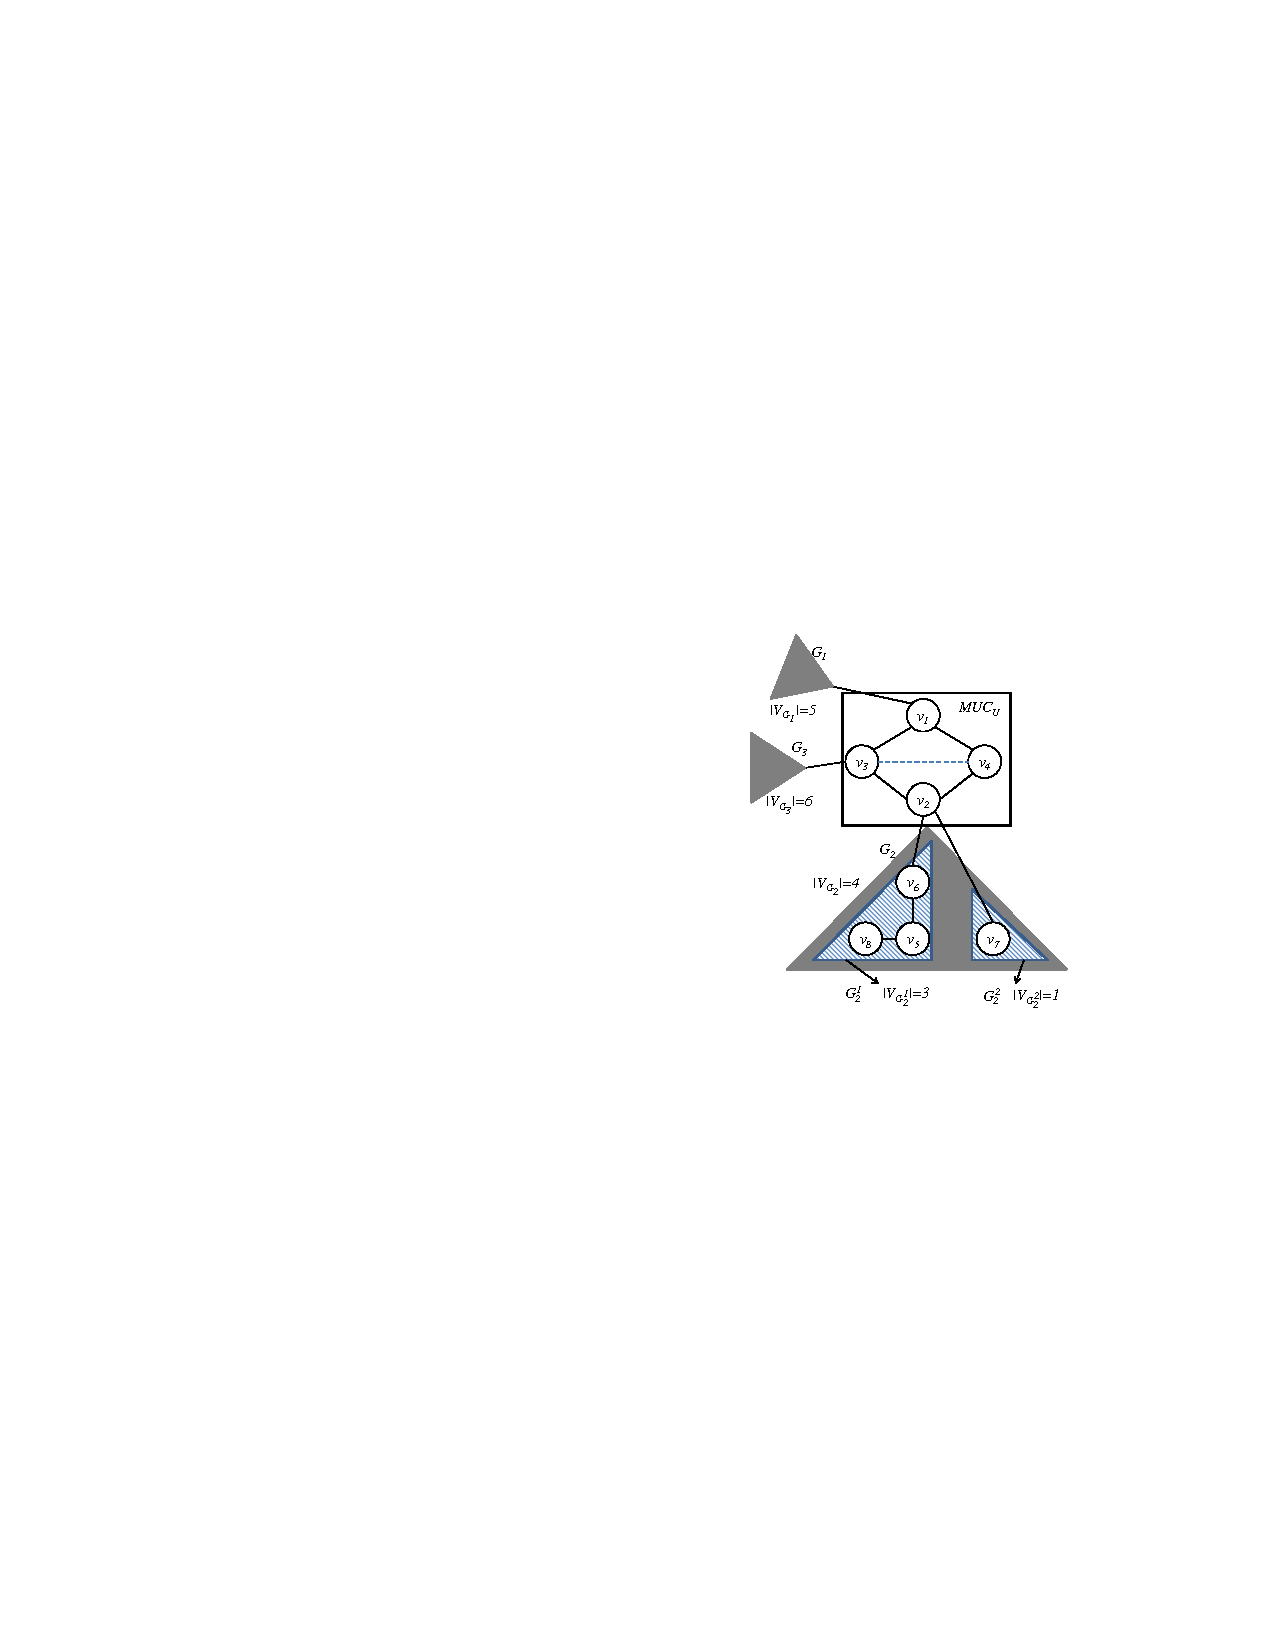
\includegraphics[width=\textwidth, height=0.8\textheight, keepaspectratio]{imgs/qube-biconnected}
      \end{figure}
    \end{column}
  \end{columns}

\end{frame}


\begin{frame}
  \frametitle{Finding MUCs}

  \begin{itemize}
    \item Finding an $MCB$ is well studied
    \item Kavitha, Mehlhorn, Michail, Paluch. ``A faster algorithm for minimum cycle basis of graphs''. ICALP 2004
    \item Finding $MUC$ from $MCB$ relatively straightforward (just union sets of vertices)
    \item Also find connection vertices for each $MUC$
    \item All done as a preprocessing step
    \item Need to be updated at runtime
  \end{itemize}
\end{frame}


\begin{frame}
  \frametitle{Updating MUCs -- Addition}

  \begin{figure}[t]
    \centering
    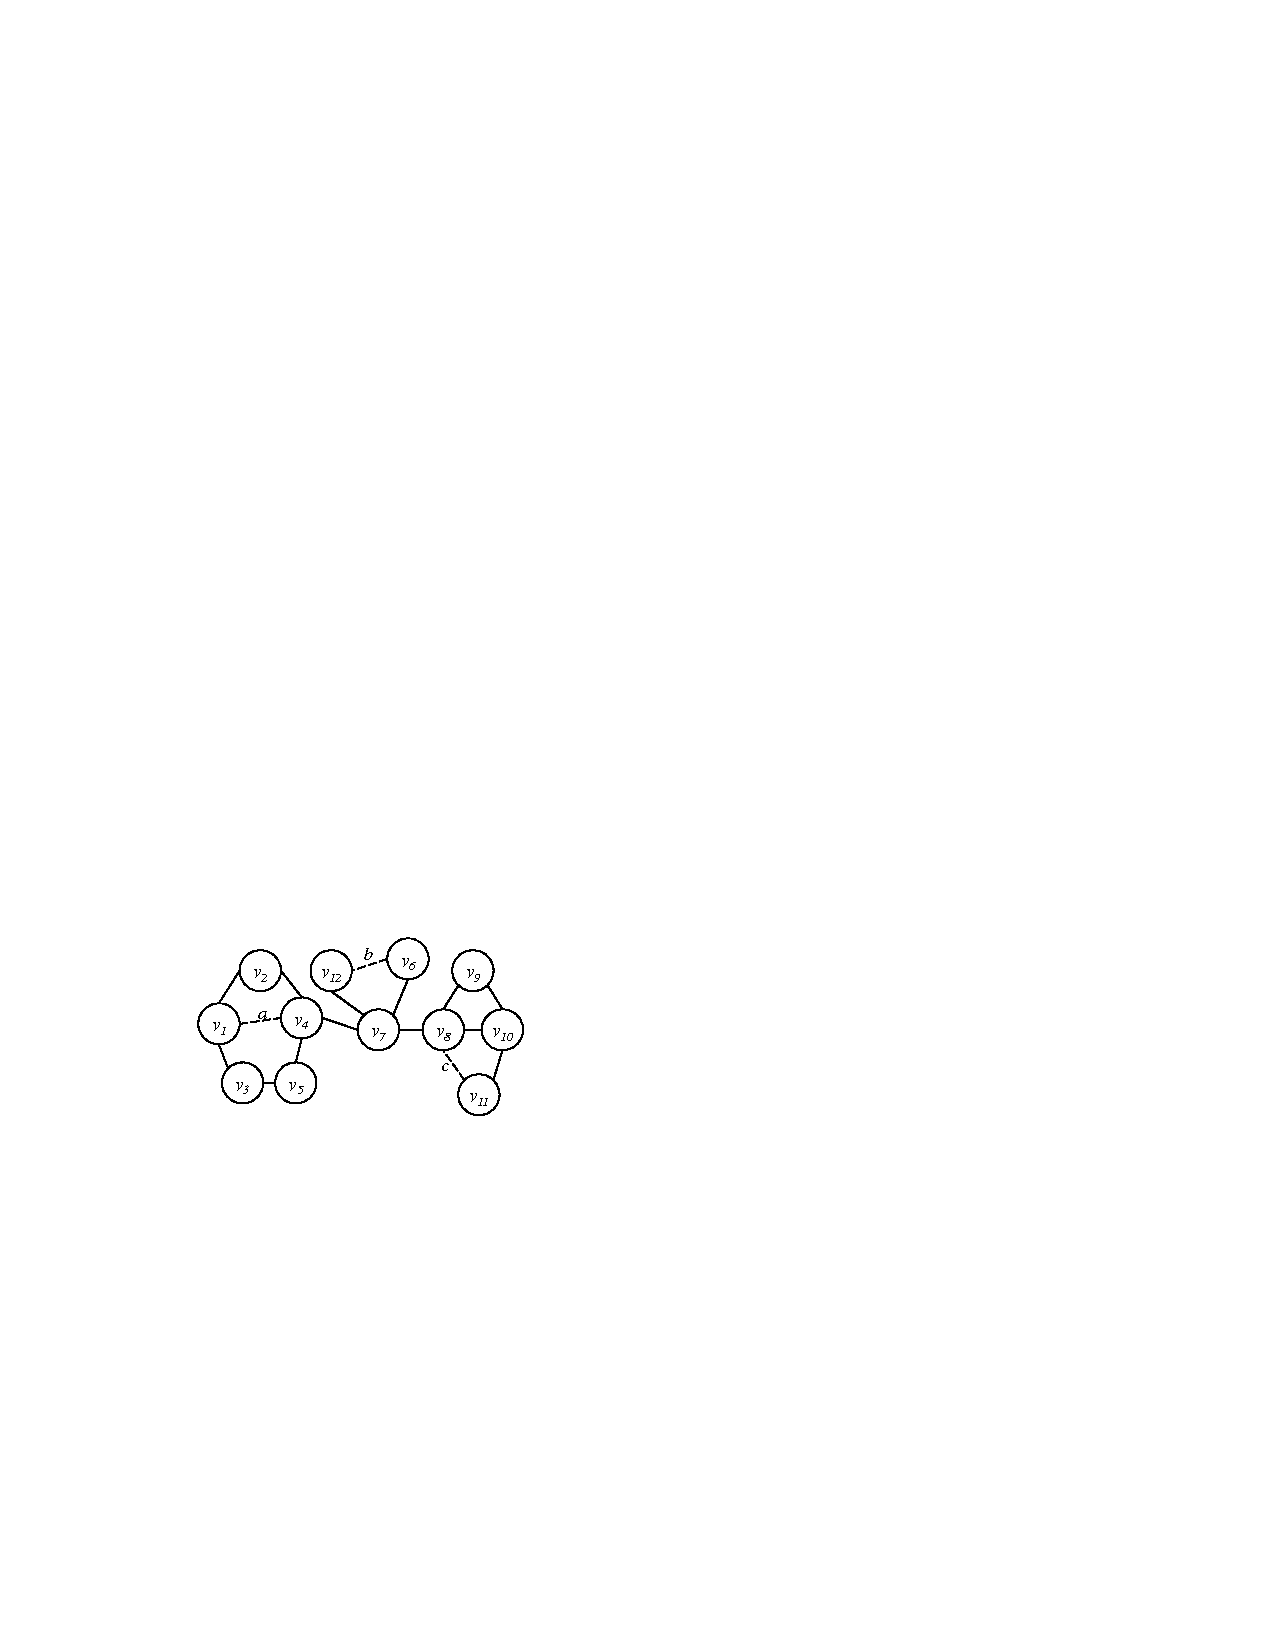
\includegraphics[width=\textwidth, height=0.6\textheight, keepaspectratio]{imgs/qube-addition}
  \end{figure}

  \begin{itemize}
    \item Adding $a$ does not affect the $MUC$ (endpoints in the same $MUC$)
    \item Adding $b$ creates a new $MUC$ (endpoints do not belong to a $MUC$)
    \item Adding $c$ merges two $MUC$s (merge $MUC$s of vertices on the \spath between endpoints)
  \end{itemize}
\end{frame}


\begin{frame}
  \frametitle{Updating MUCs -- Removal}

  \begin{figure}[t]
    \centering
    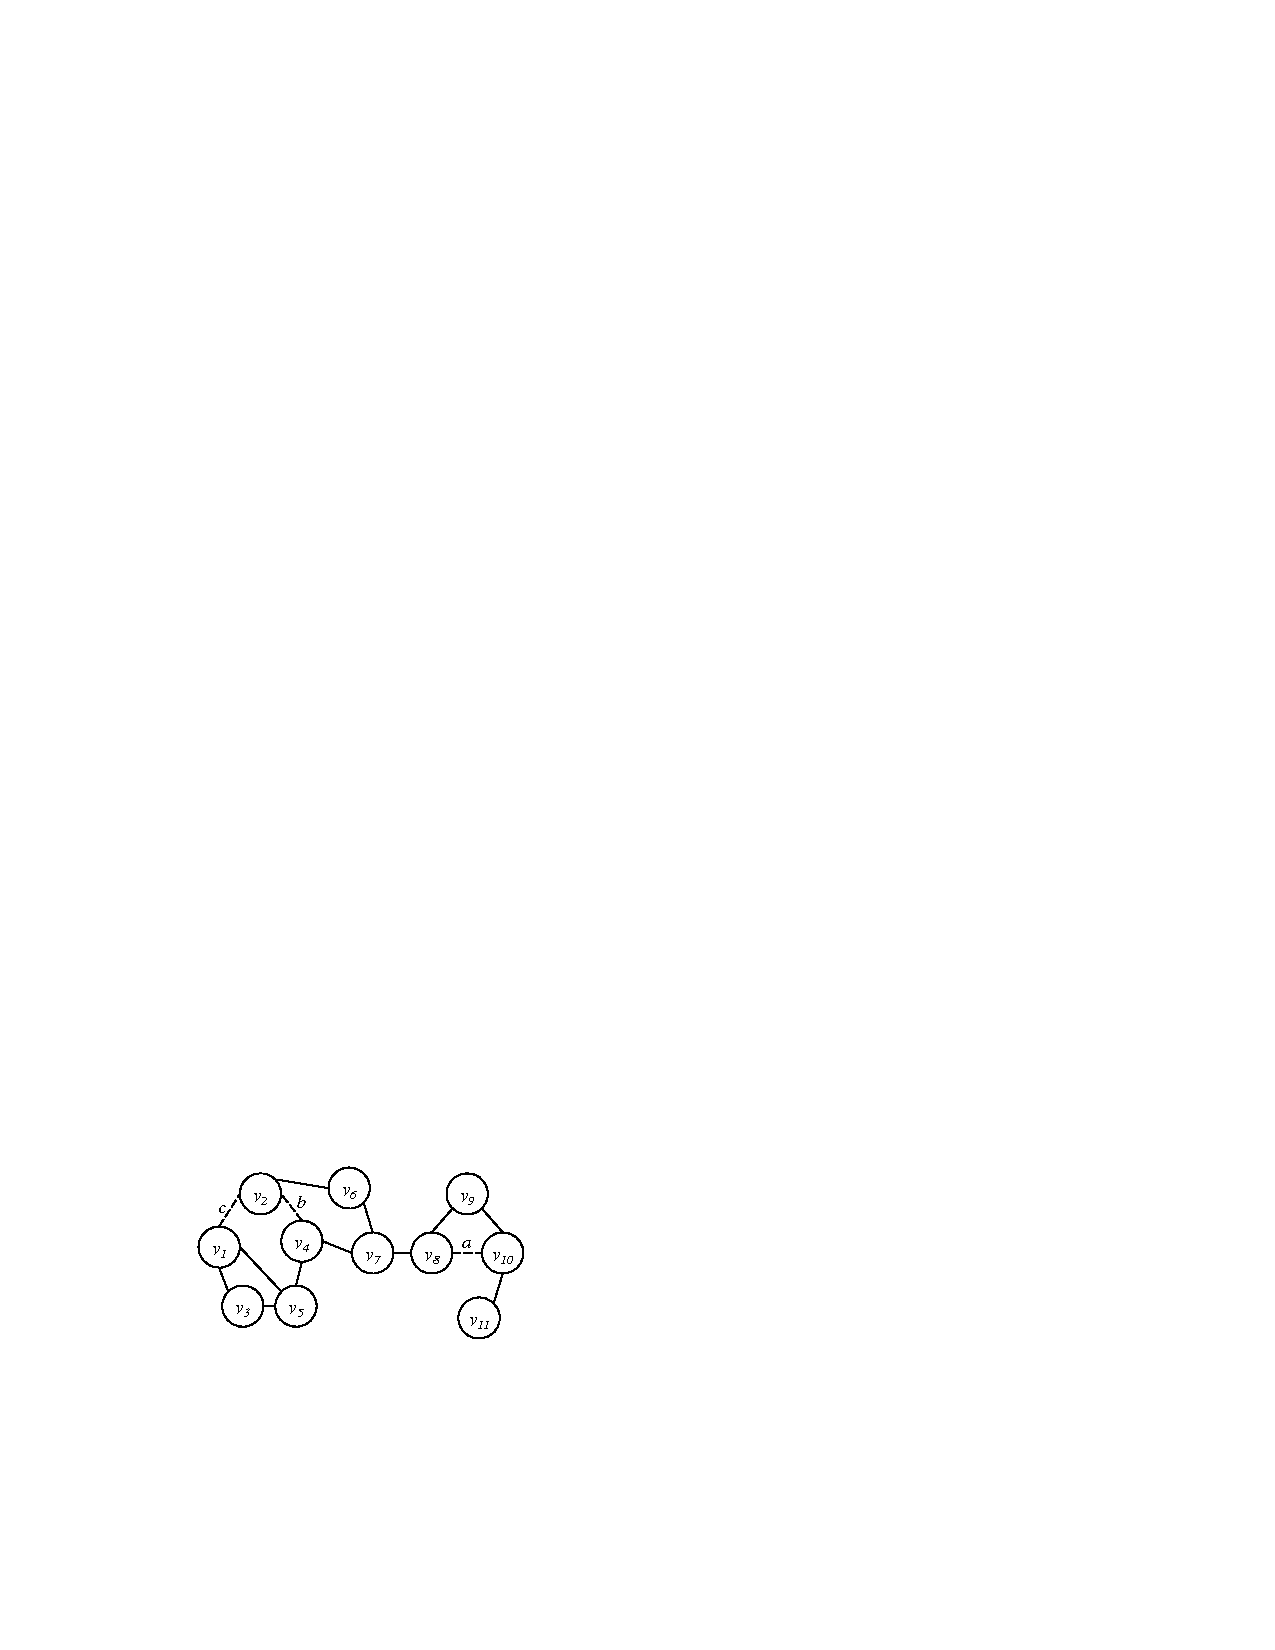
\includegraphics[width=\textwidth, height=0.6\textheight, keepaspectratio]{imgs/qube-removal}
  \end{figure}

  \begin{itemize}
    \item Removing $a$ destroys the $MUC$ (cycle is removed $\rightarrow$ no biconnected component)
    \item Removing $b$ does not affect the $MUC$ ($MUC$ is still biconnected)
    \item Removing $c$ splits the $MUC$ in two (single vertex appears in all \spath between endpoints)
  \end{itemize}
\end{frame}


\begin{frame}
  \frametitle{Betweenness Centrality Dependency}

  \begin{itemize}
    \item Only vertexes inside the $MUC$s of the updated endpoints need to be updated
    \item However, recomputing all centralities for the $MUC$ still requires new shortest paths to the rest of the graph
      \begin{itemize}
        \item Shortest paths to vertices outside the $MUC$
        \item Shortest paths that pass through the $MUC$
      \end{itemize}
  \end{itemize}

  \begin{figure}[t]
    \centering
    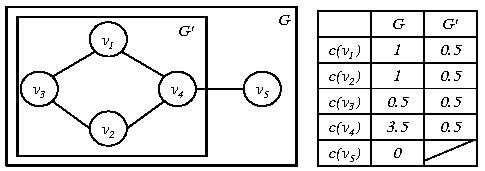
\includegraphics[width=\textwidth, height=0.6\textheight, keepaspectratio]{imgs/qube-btwmuc}
  \end{figure}
\end{frame}


\begin{frame}
  \frametitle{Betweenness Centrality outside the MUC}

  \begin{itemize}
    \item Let $s \in V_{G_j}$, $t \in MUC$,
    \item Let $j \in MUC$ be a connection vertex to subgraph $G_j$
    \item Each vertex in $\spath_{jt}$ is also in $\spath_{st}$
    \item Therefore, betweenness centrality due to vertices outside the $MUC$:
  \end{itemize}

  \begin{align*}
    %\large
    \betw_{o}(v) = \begin{cases}
      \frac{|V_{G_j}|}{\paths_{st}}		& \text{ if } v \in\{ \spath_{jt} \setminus t \} \\
      0 						& \text{ otherwise }
    \end{cases}
  \end{align*}
\end{frame}


\begin{frame}
  \frametitle{Betweenness Centrality trough the MUC}

  \begin{itemize}
    \item Let $s \in V_{G_j}$, $t \in V_{G_k}$,
    \item Let $j \in MUC$ be a connection vertex to subgraph $G_j$
    \item Let $k \in MUC$ be a connection vertex to subgraph $G_k$
    \item Each vertex in $\spath_{jk}$ is also in $\spath_{st}$
    \item Therefore, betweenness centrality due to paths through the $MUC$:
  \end{itemize}

  \begin{align*}
    \betw_{x}(v) = \begin{cases}
      \frac{ |V_{G_j}| |V_{G_k}| }{ \paths_{st} }		& \text{ if } v \in \spath_{jk} \\
      0 						& \text{ otherwise }
    \end{cases}
  \end{align*}

  More caveats apply for subgraphs that are disconnected, as every path that connects vertices in different connected component passes through $v$
\end{frame}


\begin{frame}
  \frametitle{Updating Betweenness Centrality}

  {\huge
    \begin{align*}
      \betw(v) = \betw_{MUC}(v) + \sum_{G_j \subset G} \betw_{o}(v) + \sum_{G_j, G_k \subset G} \betw_{x}(v)
    \end{align*}
  }
\end{frame}


\begin{frame}
  \frametitle{QUBE algorithm}

  \begin{figure}[t]
    \centering
    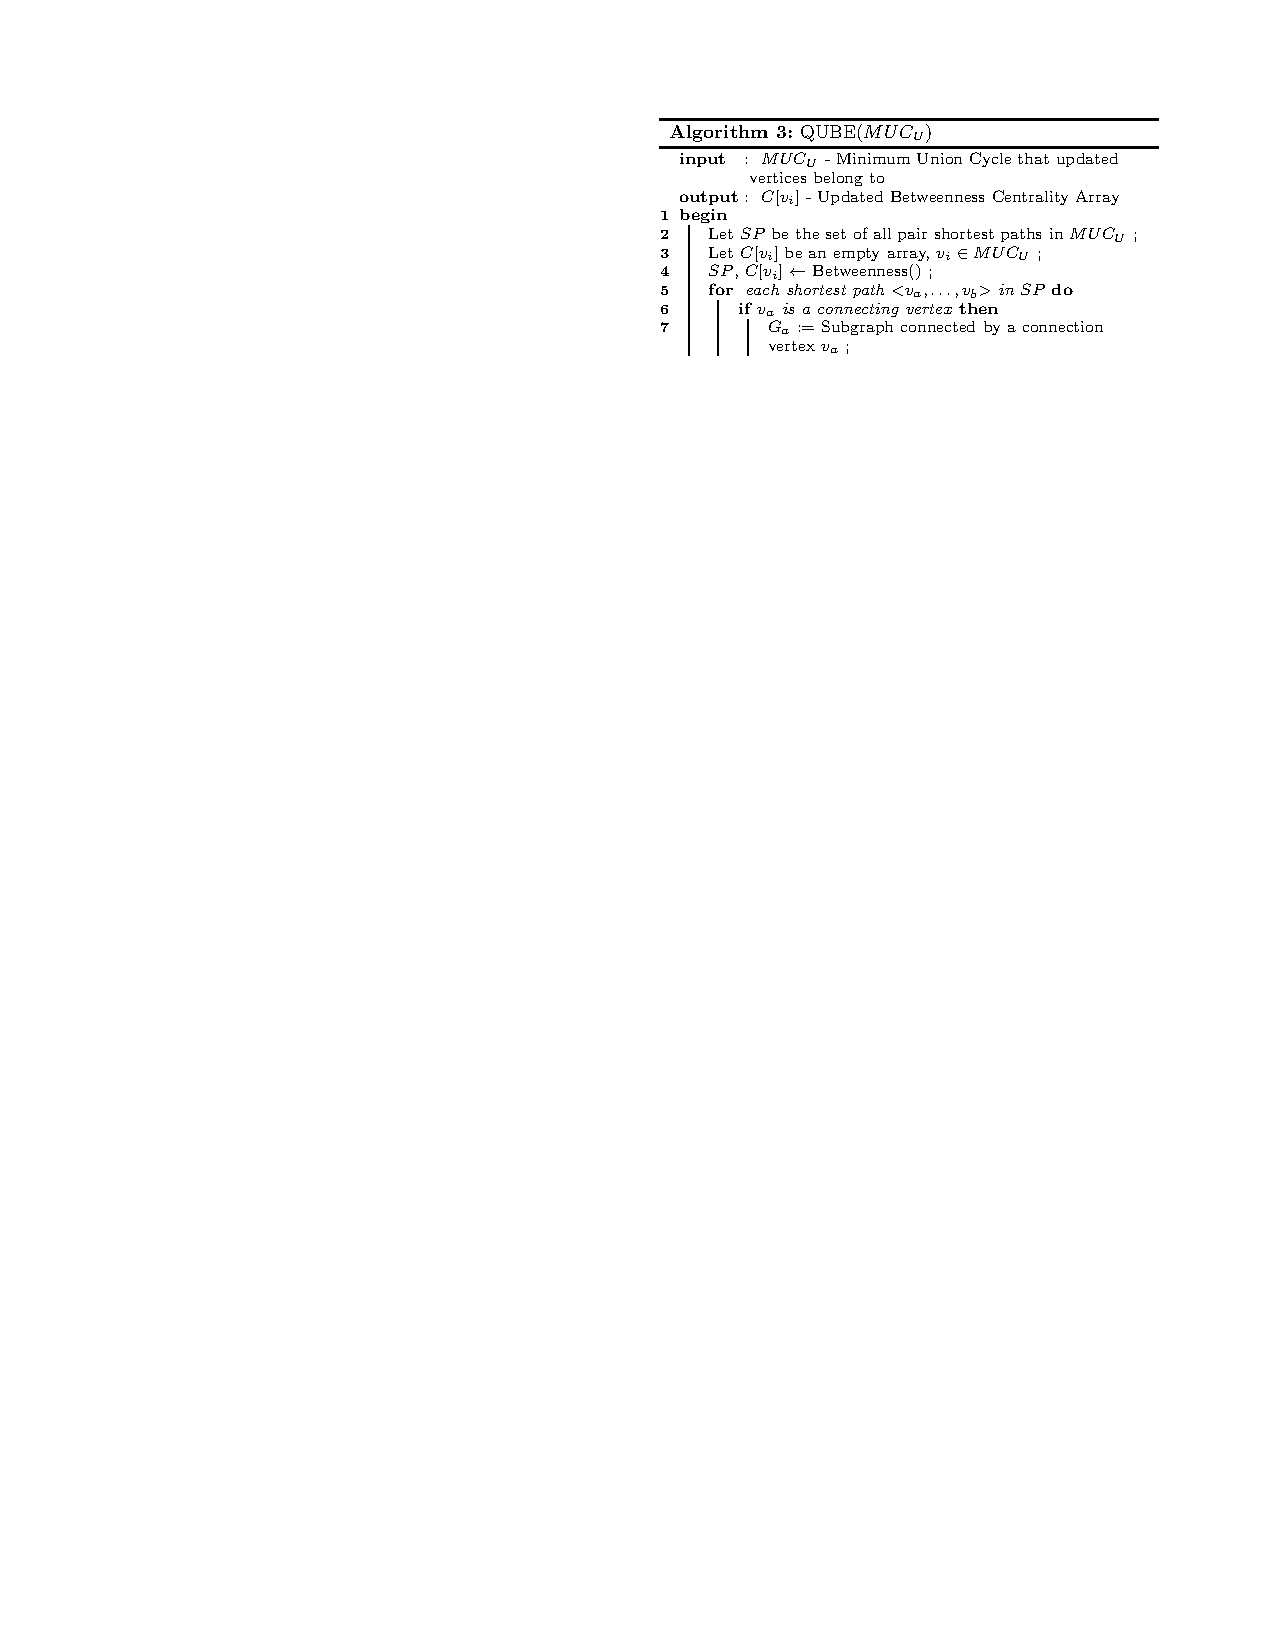
\includegraphics[width=\textwidth, height=\textheight, keepaspectratio]{imgs/qube-algorithm1}
  \end{figure}

  %  \begin{columns}[onlytextwidth]
  %    \begin{column}{0.5\textwidth}
  %      \begin{figure}[t]
  %        \centering
  %        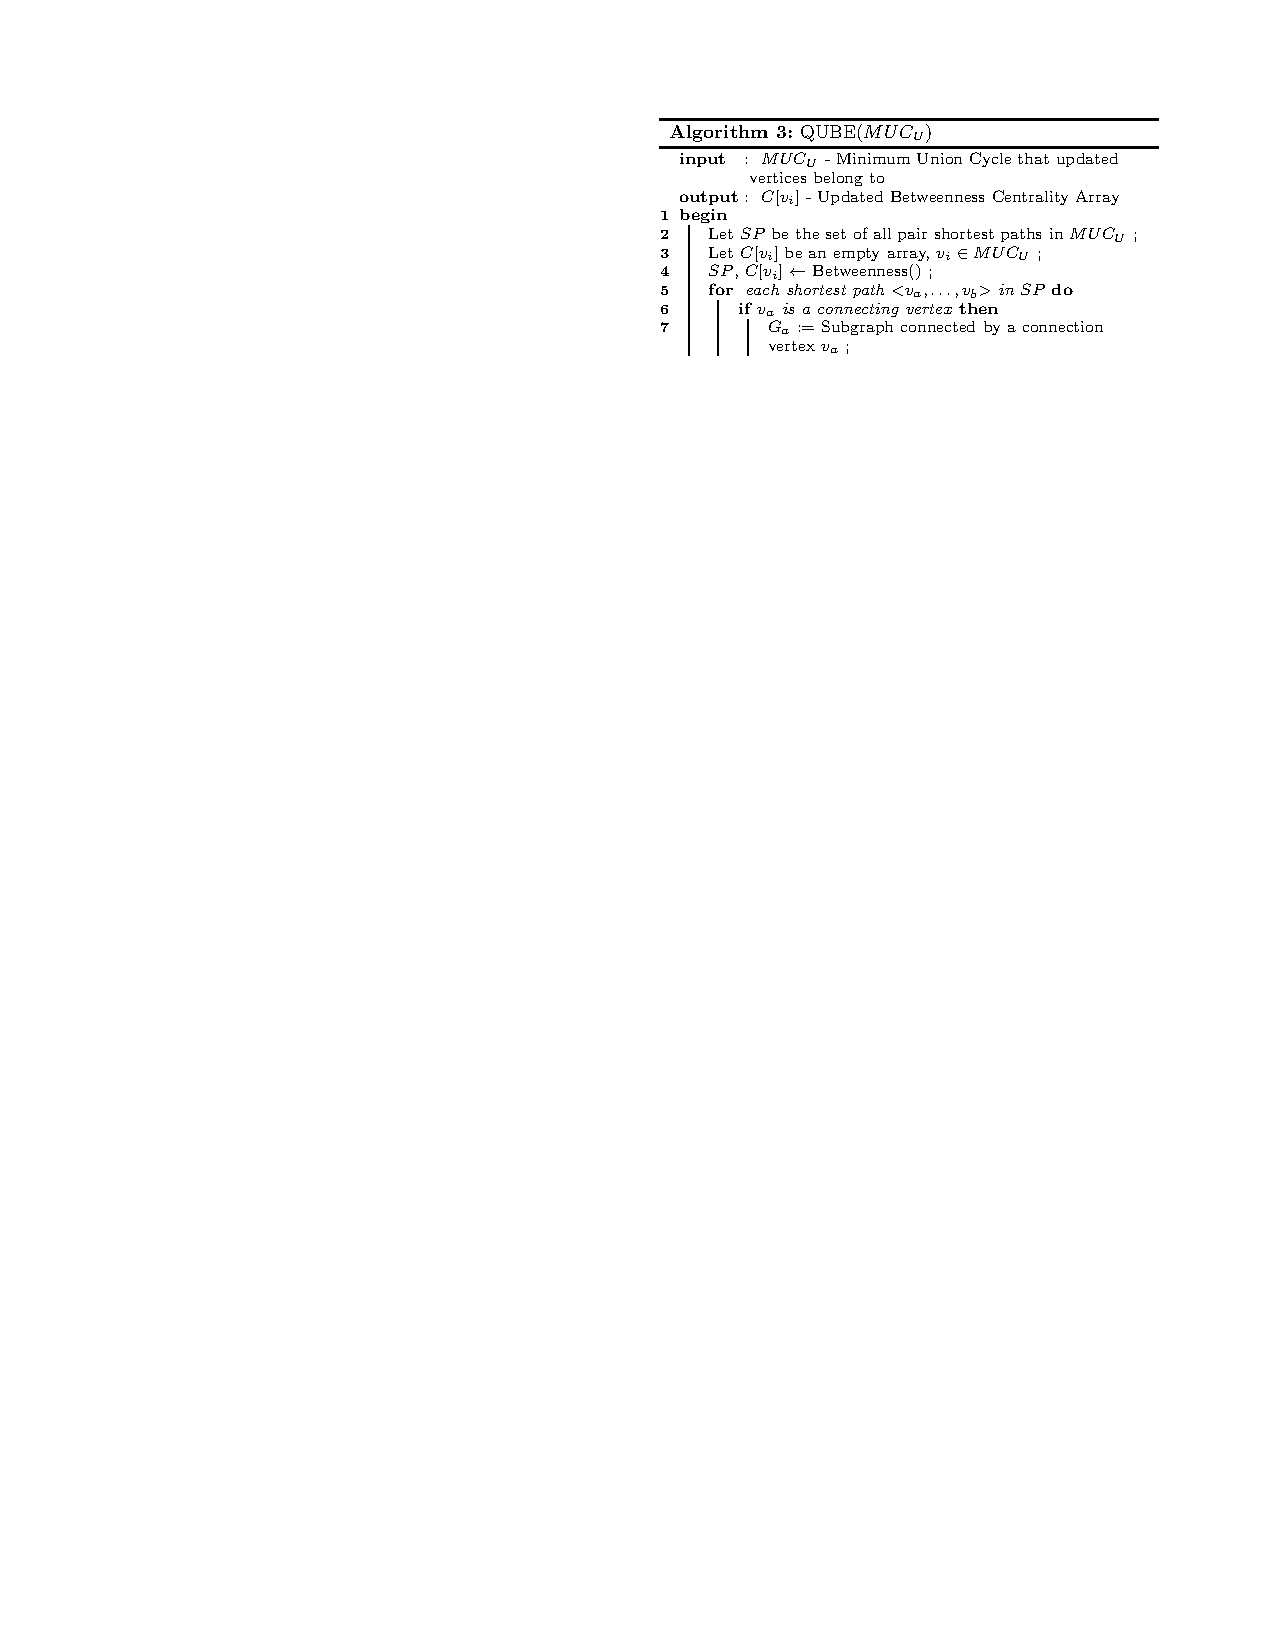
\includegraphics[width=\textwidth, height=\textheight, keepaspectratio]{imgs/qube-algorithm1}
  %      \end{figure}
  %    \end{column}

  %    \begin{column}{0.5\textwidth}
  %      \begin{figure}[t]
  %        \centering
  %        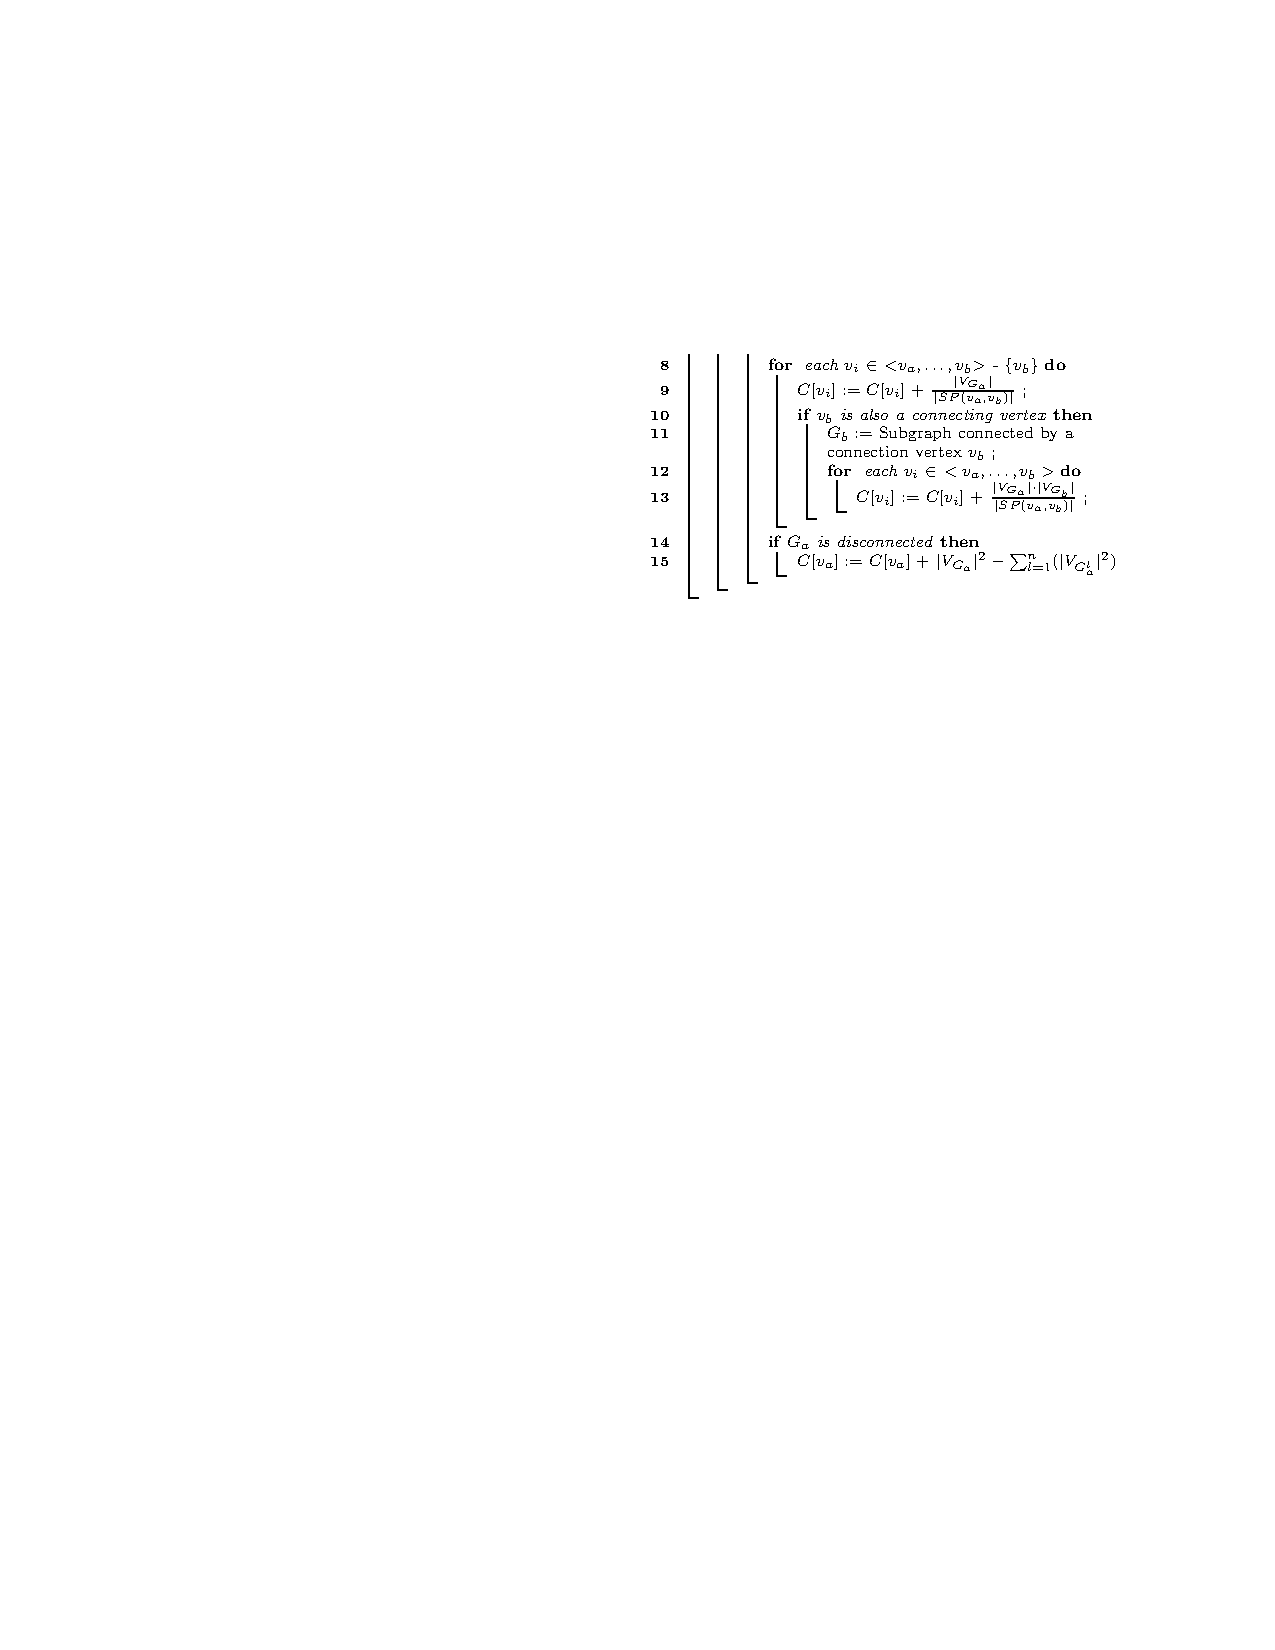
\includegraphics[width=\textwidth, height=\textheight, keepaspectratio]{imgs/qube-algorithm2}
  %      \end{figure}
  %    \end{column}
  %  \end{columns}
\end{frame}


\begin{frame}
  \frametitle{QUBE algorithm}

  \begin{figure}[t]
    \centering
    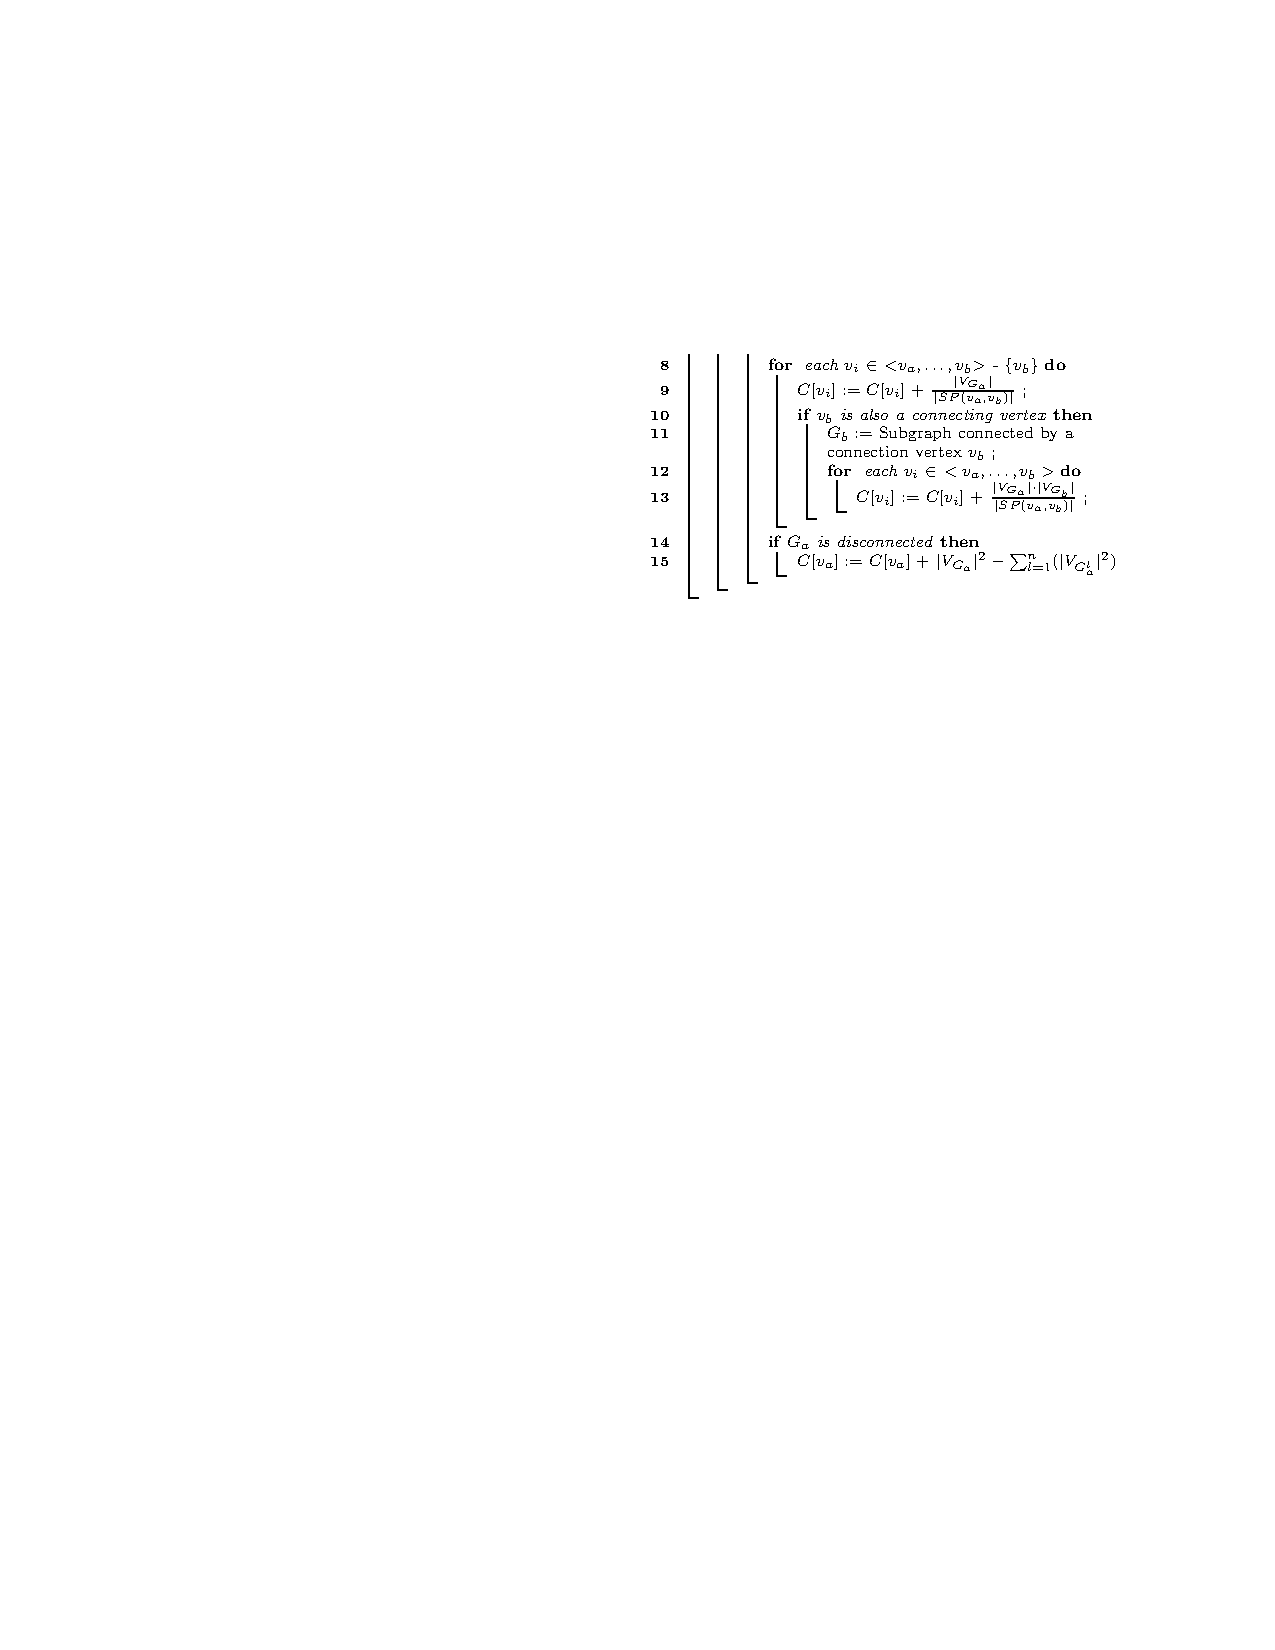
\includegraphics[width=\textwidth, height=\textheight, keepaspectratio]{imgs/qube-algorithm2}
  \end{figure}

\end{frame}


\begin{frame}
  \frametitle{QUBE + Brandes}

  \begin{itemize}
    \item QUBE is a pruning rule that reduces the search space for betweenness recomputation
    \item Can be paired with any existing betweenness algorithm to compute $\betw_{MUC}$
    \item In the experiments, Brandes' is used
    \item Quantities computed by Brandes' (e.g., \paths) reused by QUBE for $\betw_o$ and $\betw_x$
  \end{itemize}
\end{frame}


\begin{frame}
  \frametitle{Results}

  \begin{figure}[t]
    \centering
    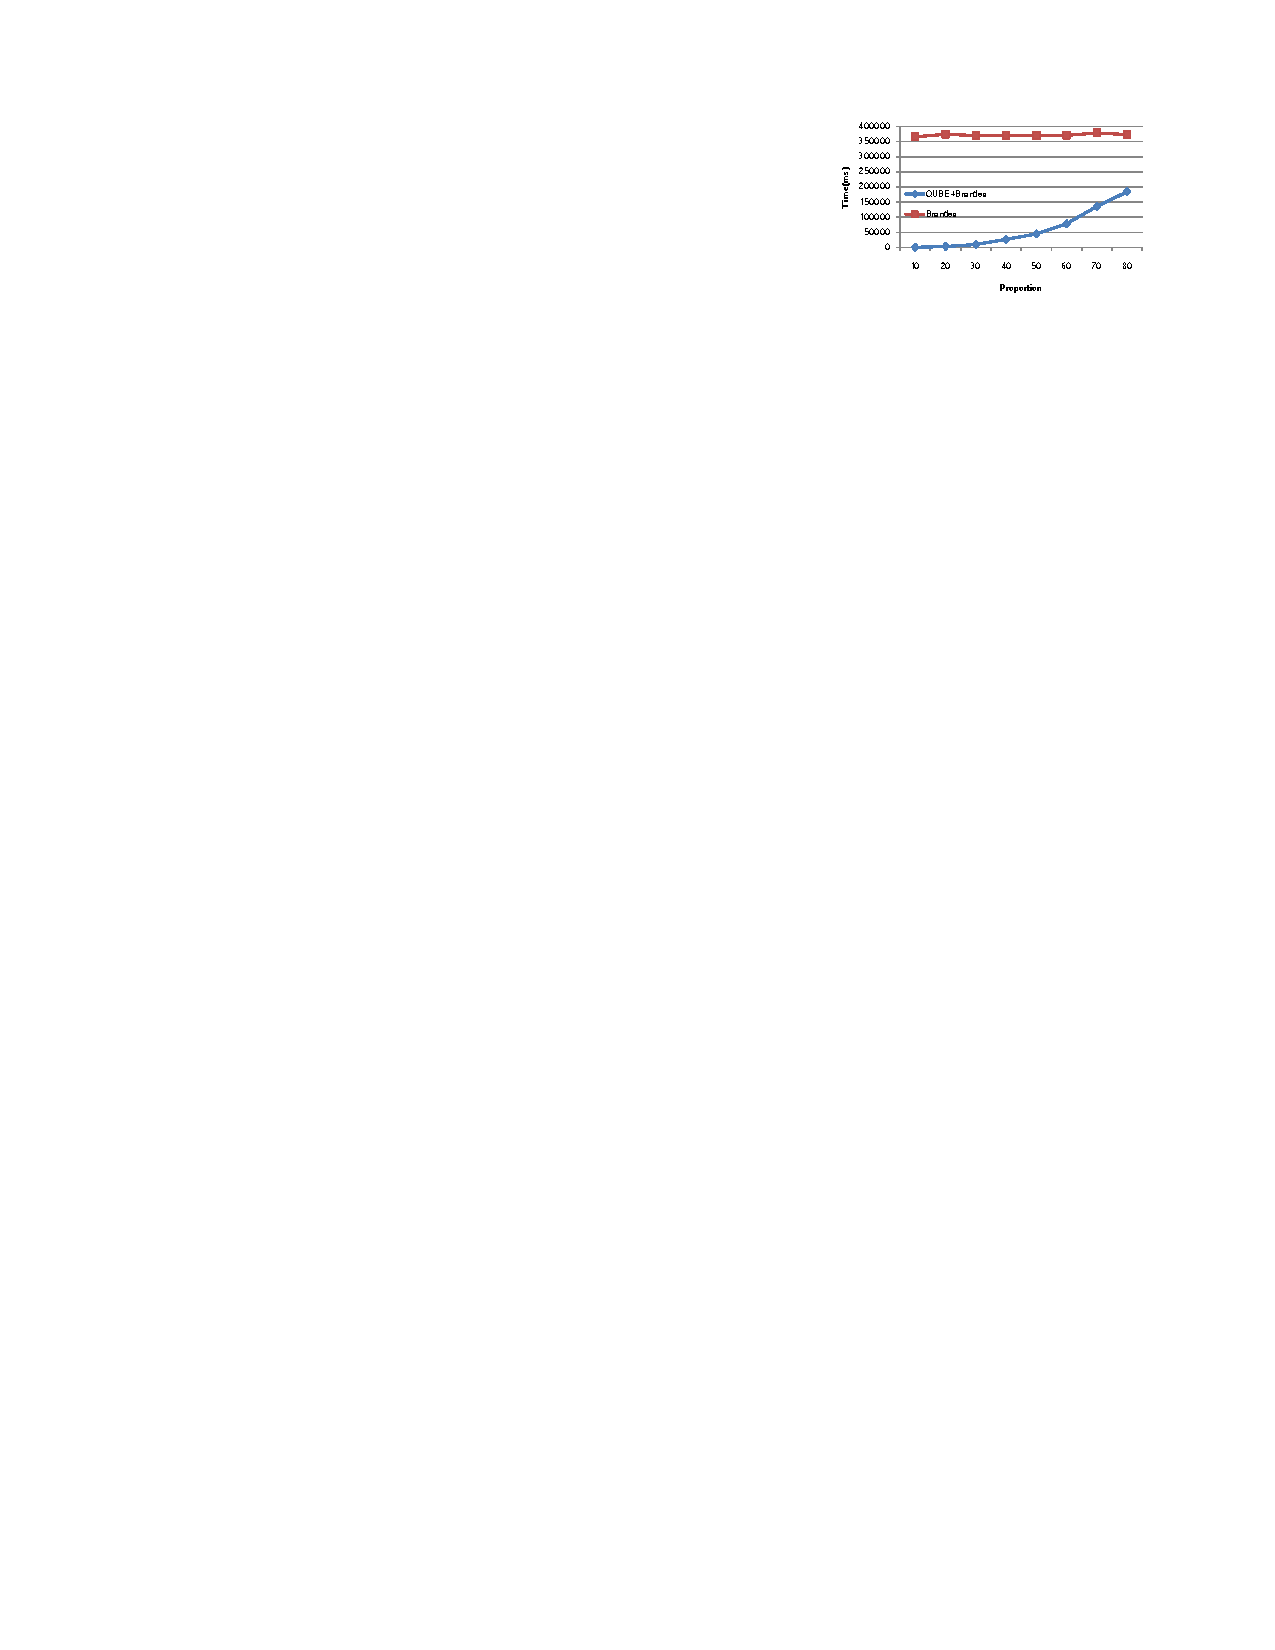
\includegraphics[width=\textwidth, height=0.7\textheight, keepaspectratio]{imgs/qube-results1}
    \caption{Update time as a function of the percentage of vertices of the graph in the updated $MUC$ for synthetic Erd\"{o}s-R\'{e}nyi graphs ($n = 5000$)}
  \end{figure}

\end{frame}


\begin{frame}
  \frametitle{Conclusions}

  \begin{figure}[t]
    \centering
    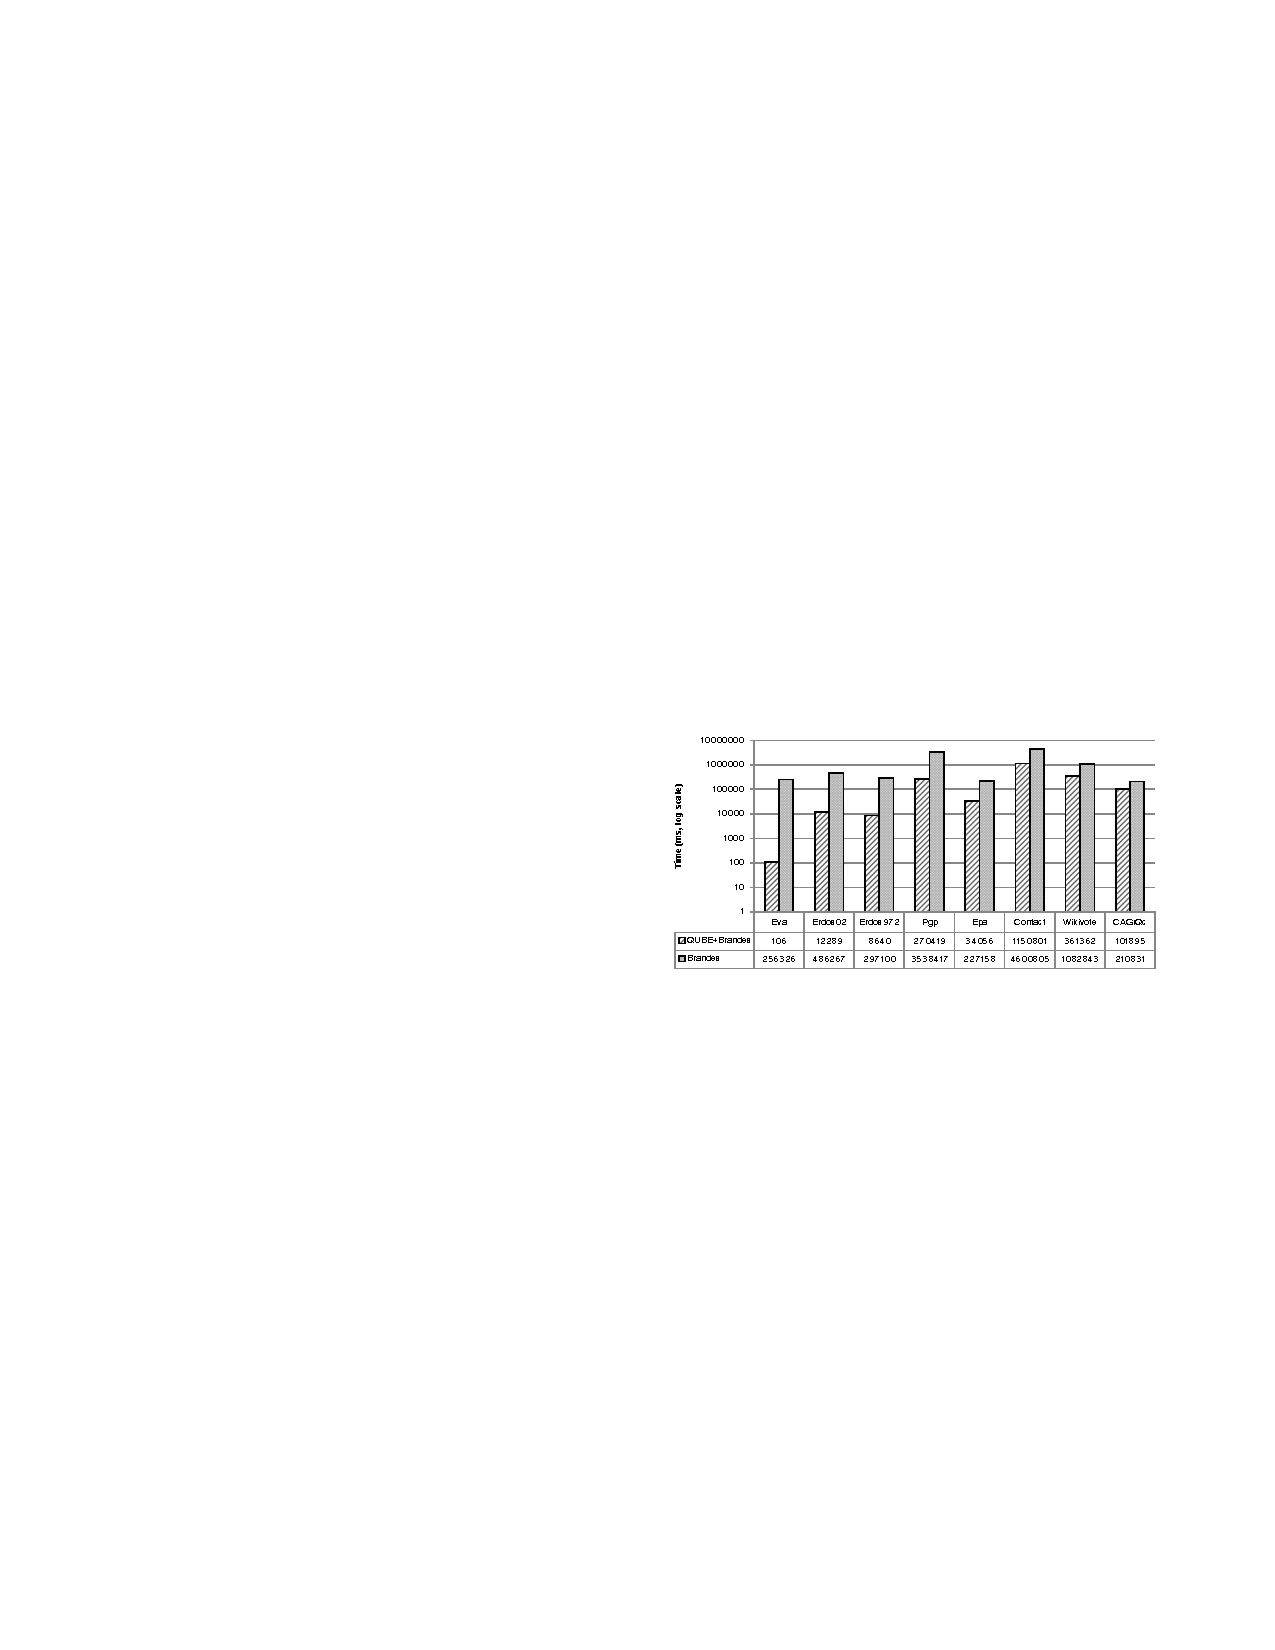
\includegraphics[width=\textwidth, height=0.6\textheight, keepaspectratio]{imgs/qube-results2}
  \end{figure}

  \begin{itemize}
    \item Improvement depends highly on structure of the graph (bi-connectedness)
    \item From 2 orders of magnitude (best) to 2 times (worst) faster than Brandes'
  \end{itemize}

\end{frame}


%% Kas et al.
\begin{frame}
  \centering
  \vfill
  {\huge Incremental Algorithm for Updating Betweenness Centrality in Dynamically Growing Networks}
  \vfill
  {\Large M. Kas, M. Wachs, K. M. Carley, L. R. Carley}
  \vfill
  {\large ASONAM '13: International Conference on Advances \\in Social Networks analysis and Mining}
  \vfill
\end{frame}


\begin{frame}
  \frametitle{Intuition}

  \begin{itemize}
    \item Extend an existing dynamic all-pairs shortest path algorithm to betweenness
    \item G. Ramalingam and T. Reps, ``\emph{On the Computational Complexity of Incremental Algorithms},'' CS, Univ. of Wisconsin at Madison, Tech. Report 1991
    \item Relevant quantities: number of shortest paths \paths, distances \dist, predecessors \pred
    \item Keep a copy of the old quantities while updating
    \item Support only edge addition (on weighted graphs)
  \end{itemize}

\end{frame}


\begin{frame}
  \frametitle{Edge update}

  \begin{itemize}
    \item Compute new shortest paths from updated endpoints $(u,v)$
    \item If a new shortest path of the same length is found, updated number of paths as
  \end{itemize}
  {\Large
    \begin{align*}
      \paths_{st} = \paths_{st} + \paths_{su} \times \paths_{vt}
    \end{align*}
  }
  \begin{itemize}
    \item If a new \emph{shorter} shortest path to any vertex is found, update \dist, clear \paths
    \item Betweenness decreased if new shortest path found
    \item Edge betweenness updates backtrack via DFS over $\pred_s(t)$
  \end{itemize}
  {\Large
    \begin{align*}
      \betw(w) = \betw(w) - \paths_{sw} \times \paths_{wt} / \paths_{st}
    \end{align*}
  }
\end{frame}


\begin{frame}
  \frametitle{Edge update}

  \begin{itemize}
    \item Complex bookkeeping: need to consider all affected vertices which have new alternative shortest paths of equal length (not covered in the original algorithm)
    \item Amend \pred during update propagation $\rightarrow$ concurrent changes to the \spdag
    \item Need to track now-unreachable vertices separately
  \end{itemize}

  \begin{itemize}
    \item After having fixed \dist, \paths, \betw, increase \betw due to new paths
    \item Update needed $\forall s,t \in V$ affected by changes (tracked from previous phase)
    \item Betweenness increase analogous to above decrease
  \end{itemize}
\end{frame}


\begin{frame}
  \frametitle{Results}

  \begin{figure}[t]
    \centering
    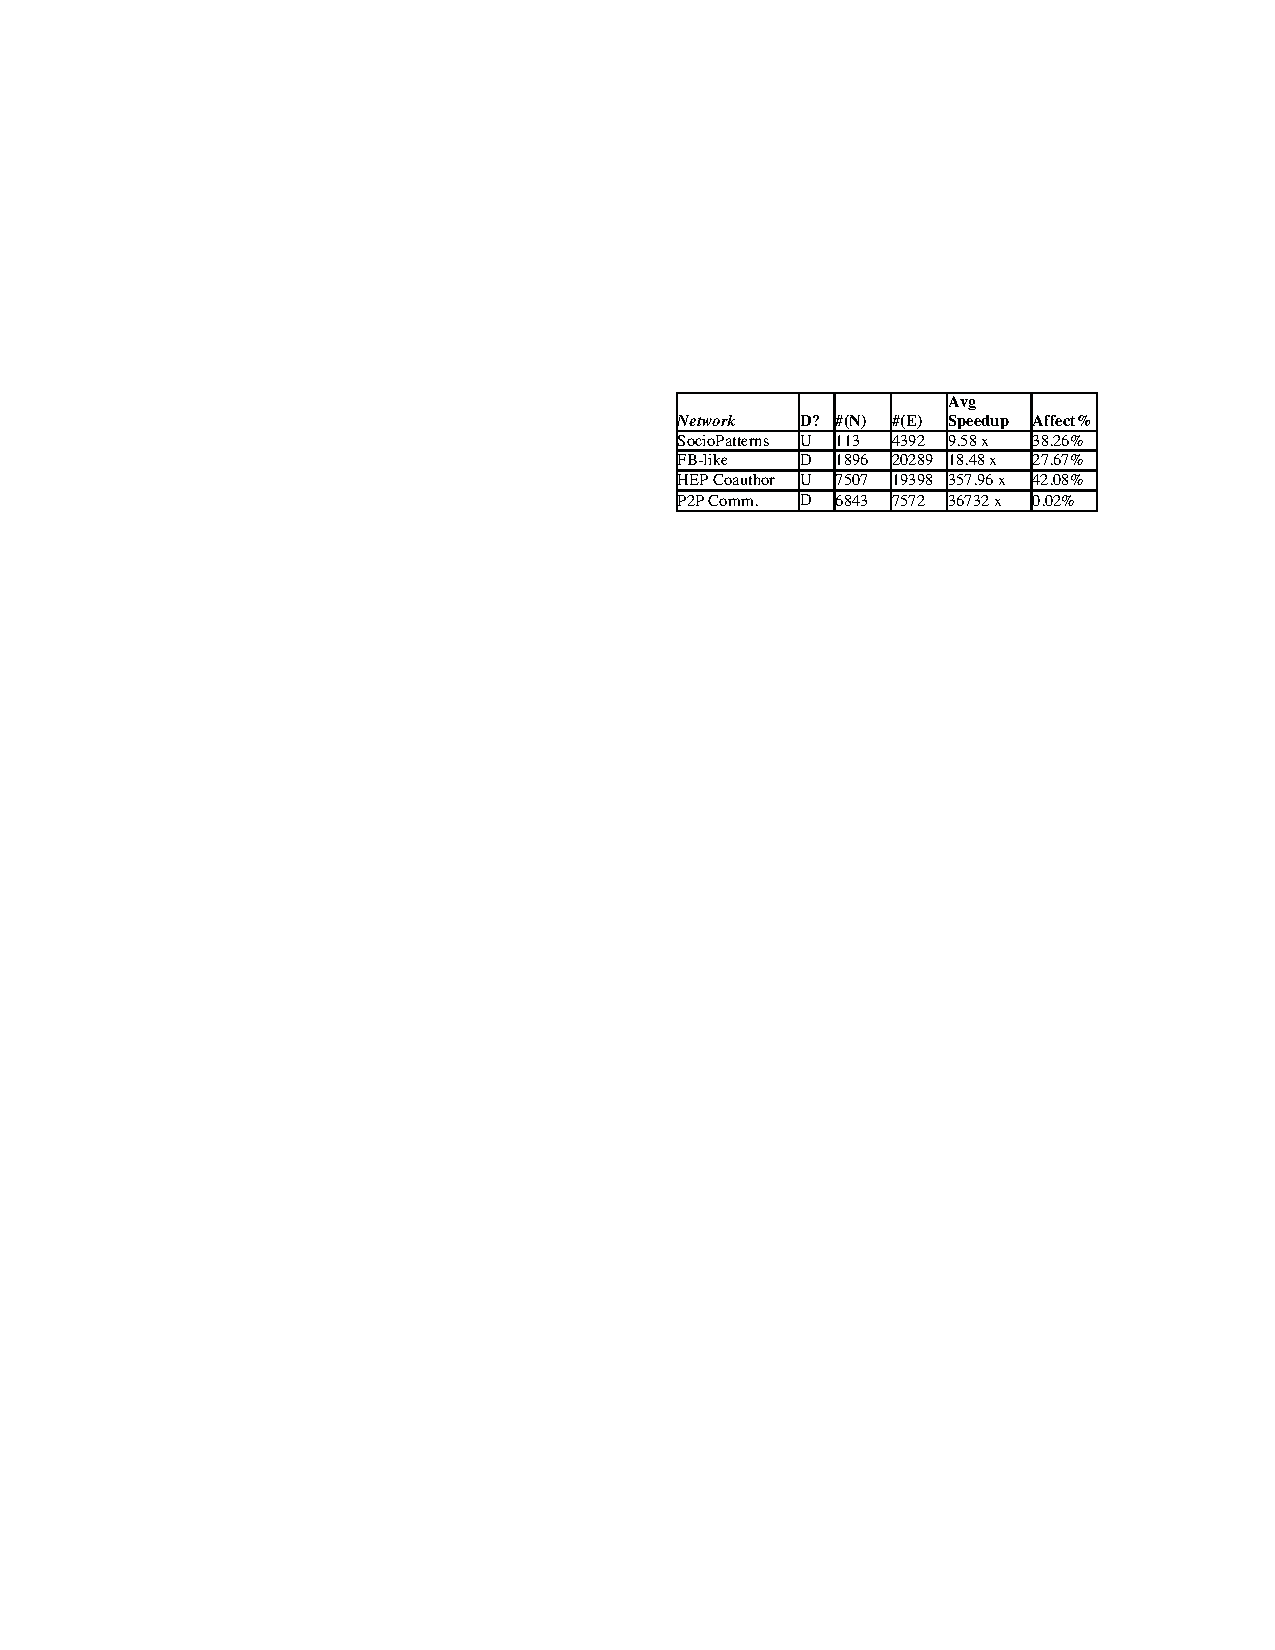
\includegraphics[width=\textwidth, height=0.7\textheight, keepaspectratio]{imgs/kas-results1}
    \caption{Speedup over Brandes' on real-world graphs}
  \end{figure}

  \begin{itemize}
    \item Speedup depends on topological characteristics (e.g., diameter, clust. coeff.)
  \end{itemize}

\end{frame}


\begin{frame}
  \frametitle{Comparison with QUBE}

  \begin{figure}[t]
    \centering
    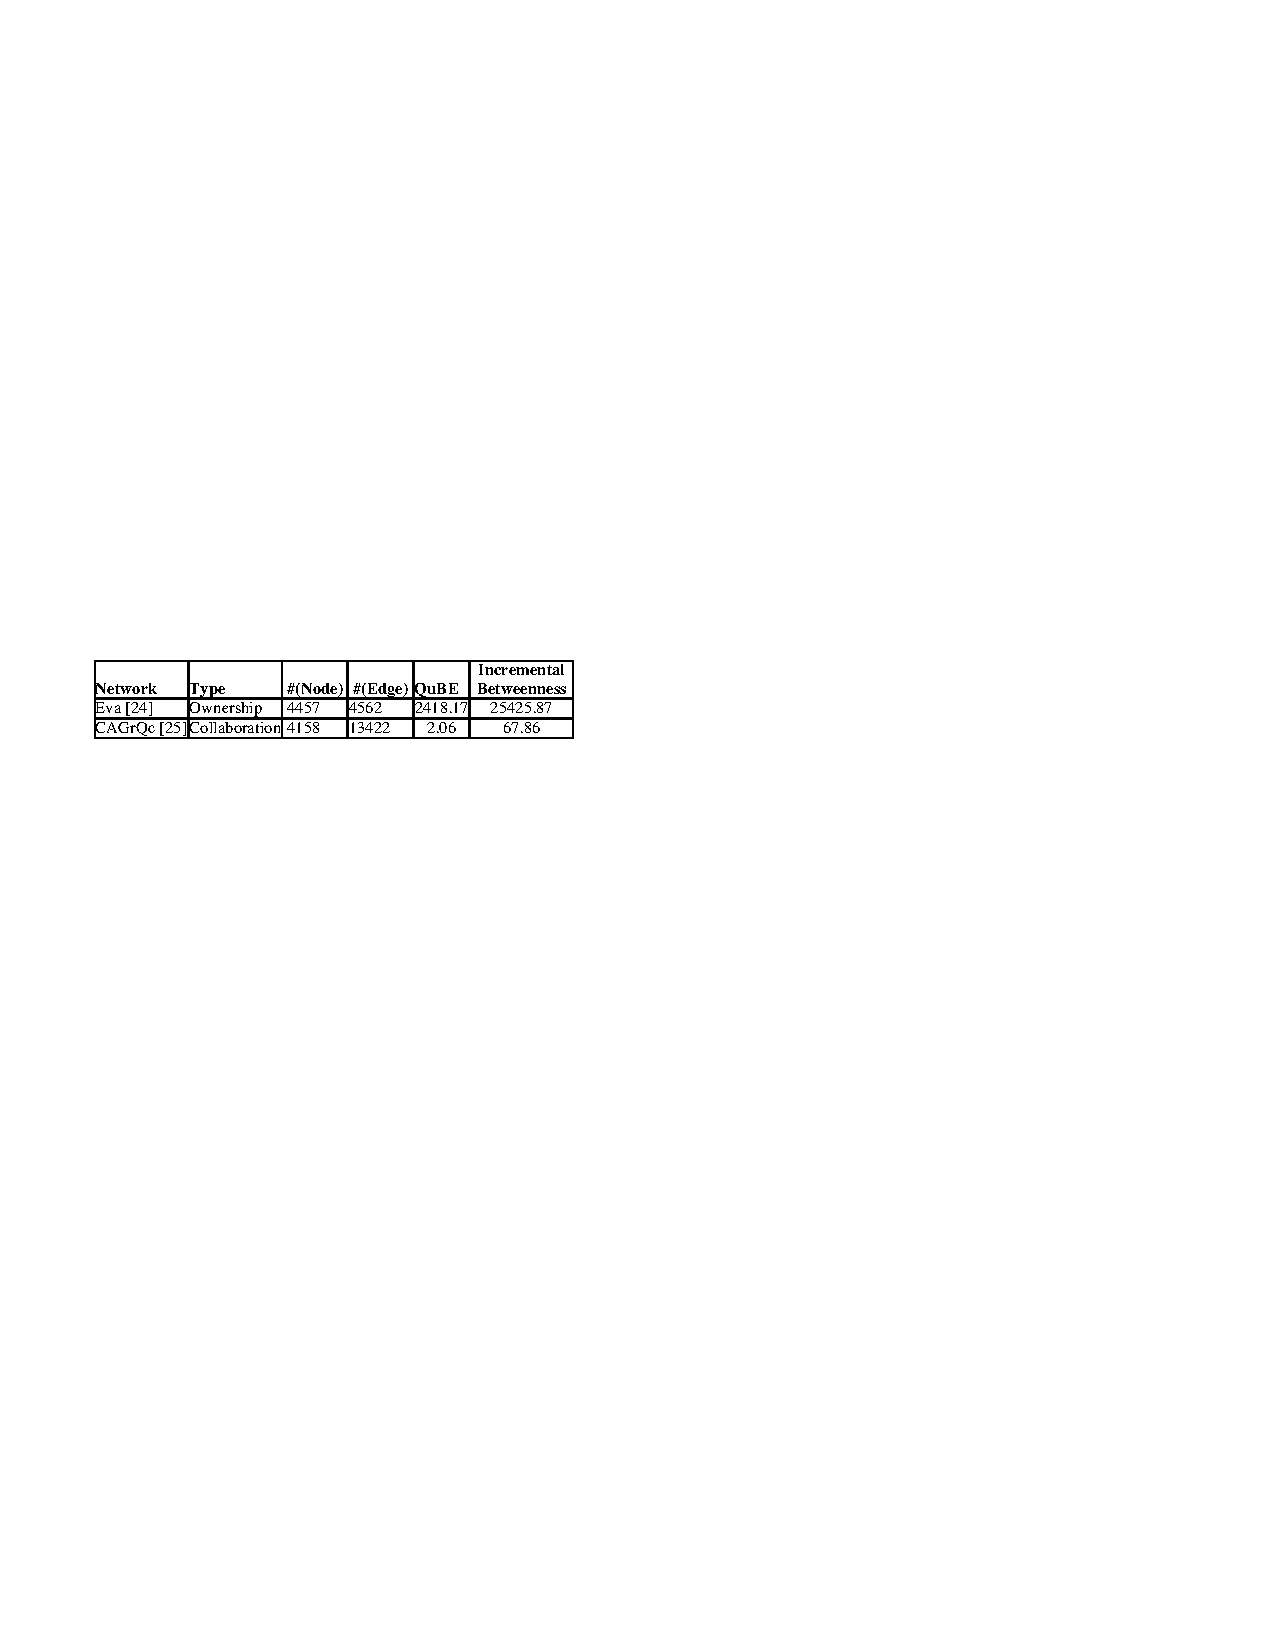
\includegraphics[width=\textwidth, height=0.7\textheight, keepaspectratio]{imgs/kas-results2}
    \caption{Speedup over Brandes' in comparison with QUBE}
  \end{figure}

  \begin{itemize}
    \item Datasets from the QUBE paper
    \item About 1 order of magnitude faster than QUBE
  \end{itemize}

\end{frame}


%% Nasre et al.
\begin{frame}
  \centering
  \vfill
  {\huge Betweenness Centrality -- Incremental and Faster}
  \vfill
  {\Large M. Nasre, M. Pontecorvi, V. Ramachandran}
  \vfill
  {\large MFCS '14: Mathematical Foundations of Computer Science}
  \vfill
\end{frame}


\begin{frame}
  \frametitle{Intuition}

  \begin{itemize}
    \item Keep \spdag for each vertex
    \item Re-use information from \spdag of updated edge endpoints
    \item Adding new edges will \emph{not} make old edges part of a \spath
    \item Support only edge addition (on weighted graphs)
  \end{itemize}

\end{frame}


\begin{frame}
  \frametitle{Main Result}

  %  \begin{figure}[H]
  %    \centering
  %    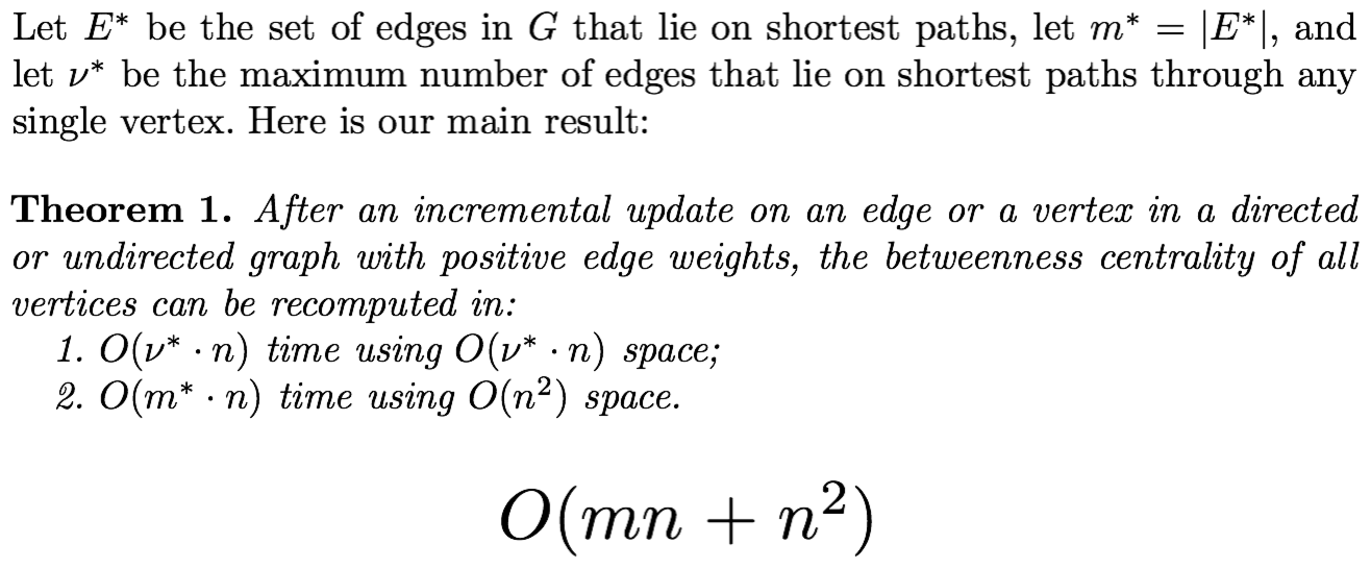
\includegraphics[width=0.5\textwidth]{imgs/npr14-main-result}
  %  \end{figure}

  \begin{itemize}
    \item Let $\displaystyle E^* = \bigcup_{e \in \allspath} e \subseteq E$ be the set of edges that are part of any shortest path
    \item Let $\displaystyle m^* = |E^*|$ and $\displaystyle \nu^* = \max_{v \in V} |\spdag_v|$ the maximum number of edges in shortest paths through any single vertex $v$
    \item $n < \nu^* < m^* < m$
    \item After incremental update, betweenness can be recomputed in
      \begin{itemize}
        \item $O(\nu^* n)$ time using $O(\nu^* n)$ space
        \item $O(m^* n)$ time using $O(n^2)$ space
      \end{itemize}
    \item Bounded by $O(mn + n^2)$
    \item Logarithmic factor better than Brandes' (on weighted graphs)
  \end{itemize}
\end{frame}


\begin{frame}
  \frametitle{Lemma 1}

  \begin{figure}[H]
    \centering
    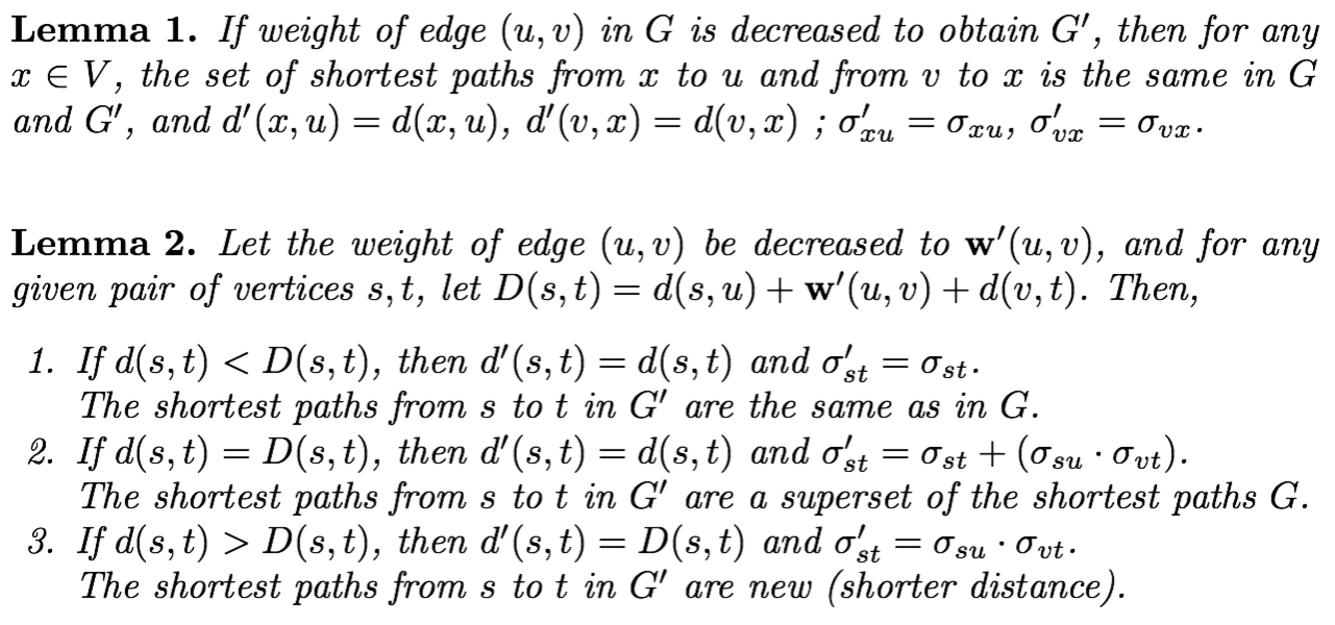
\includegraphics[width=\textwidth, trim={0 8cm 0 0}, clip]{imgs/npr14-lemmas}
  \end{figure}

  \begin{itemize}
    \item Edge $(u,v) \not\in \spath_{xu} \, \wedge \, (u,v)\not\in \spath_{vx}$ as edge weights are positive
  \end{itemize}
\end{frame}


\begin{frame}
  \frametitle{Lemma 2}

  \begin{figure}[H]
    \centering
    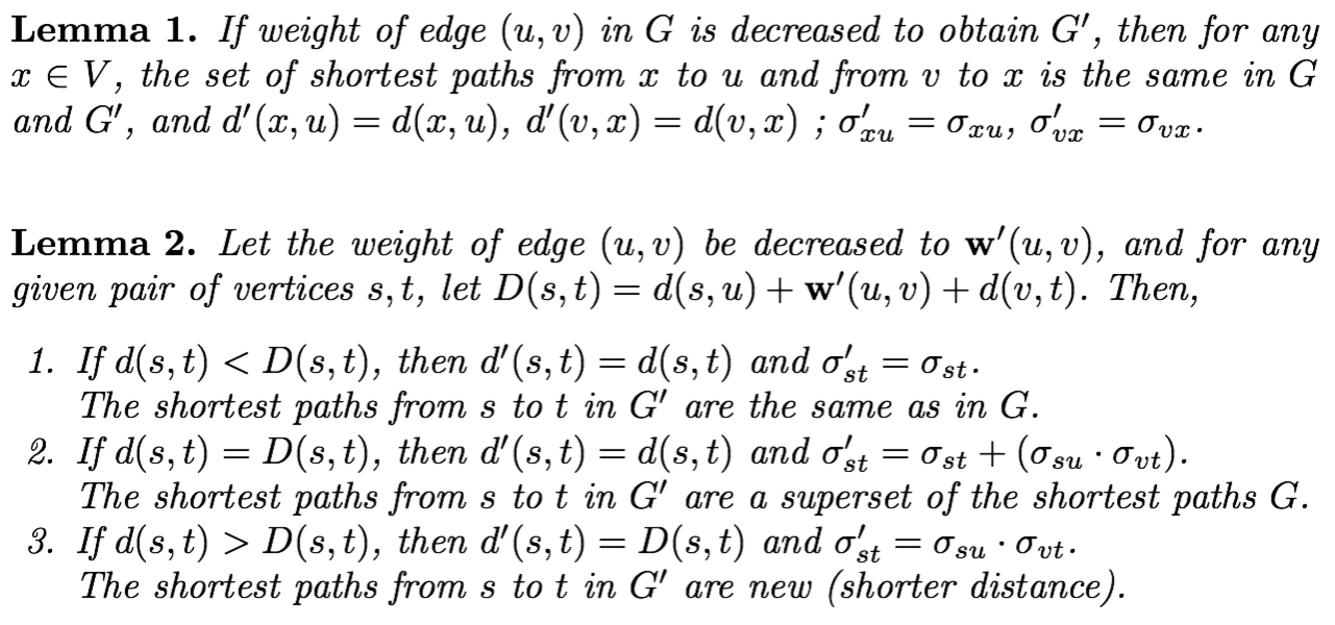
\includegraphics[width=\textwidth, trim={0 0 0 3.5cm}, clip]{imgs/npr14-lemmas}
  \end{figure}

  \begin{itemize}
    \item Updates to \paths and \dist in constant time
    \item Need to update \pred to complete \spdag update
  \end{itemize}
\end{frame}


\begin{frame}
  \frametitle{\spdag Update}

  \begin{figure}[H]
    \centering
    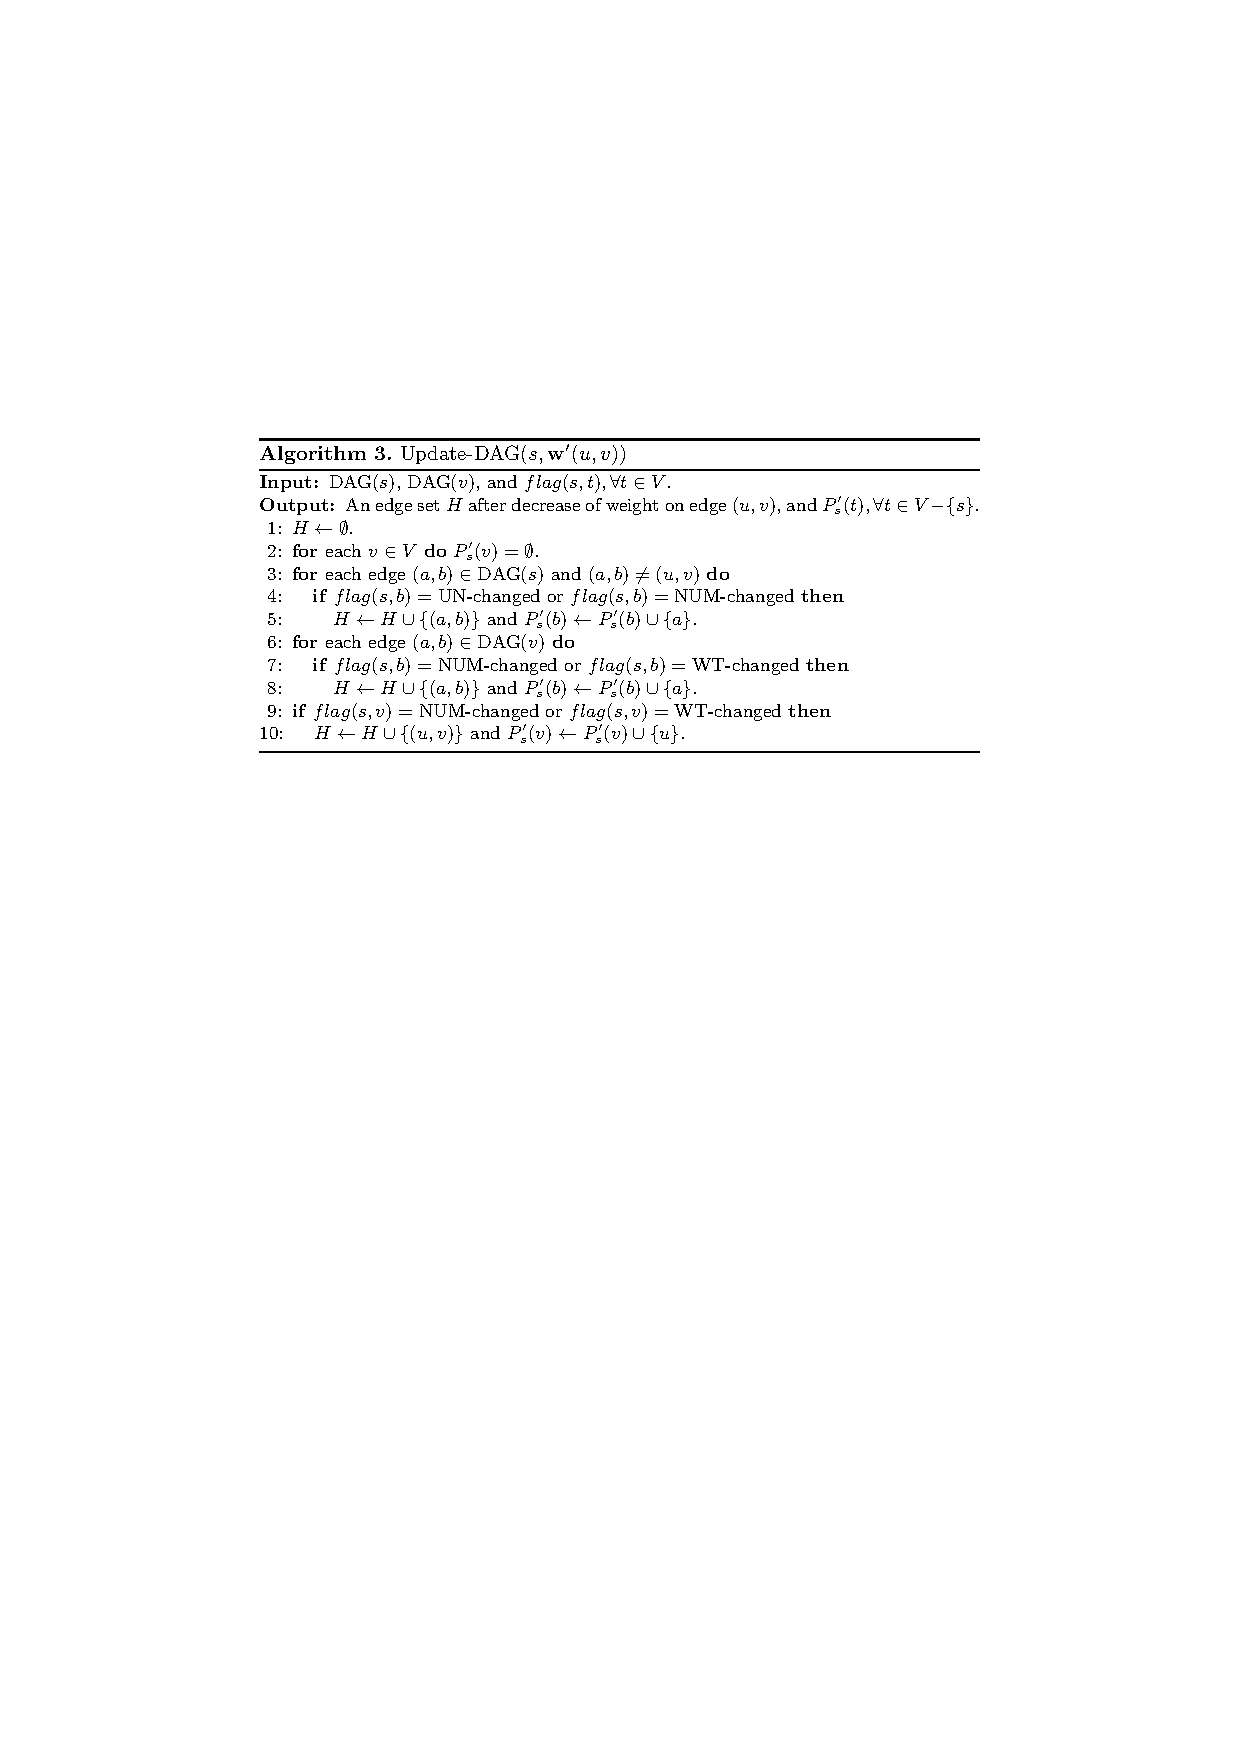
\includegraphics[width=\textwidth]{imgs/npr14-algo3}
  \end{figure}

  \begin{itemize}
    \item UN-changed $\rightarrow dd=0$, NUM-changed $\rightarrow dd=1$, WT-changed $\rightarrow dd>1$
  \end{itemize}
\end{frame}


\begin{frame}
  \frametitle{Edge Update}

  \begin{figure}[H]
    \centering
    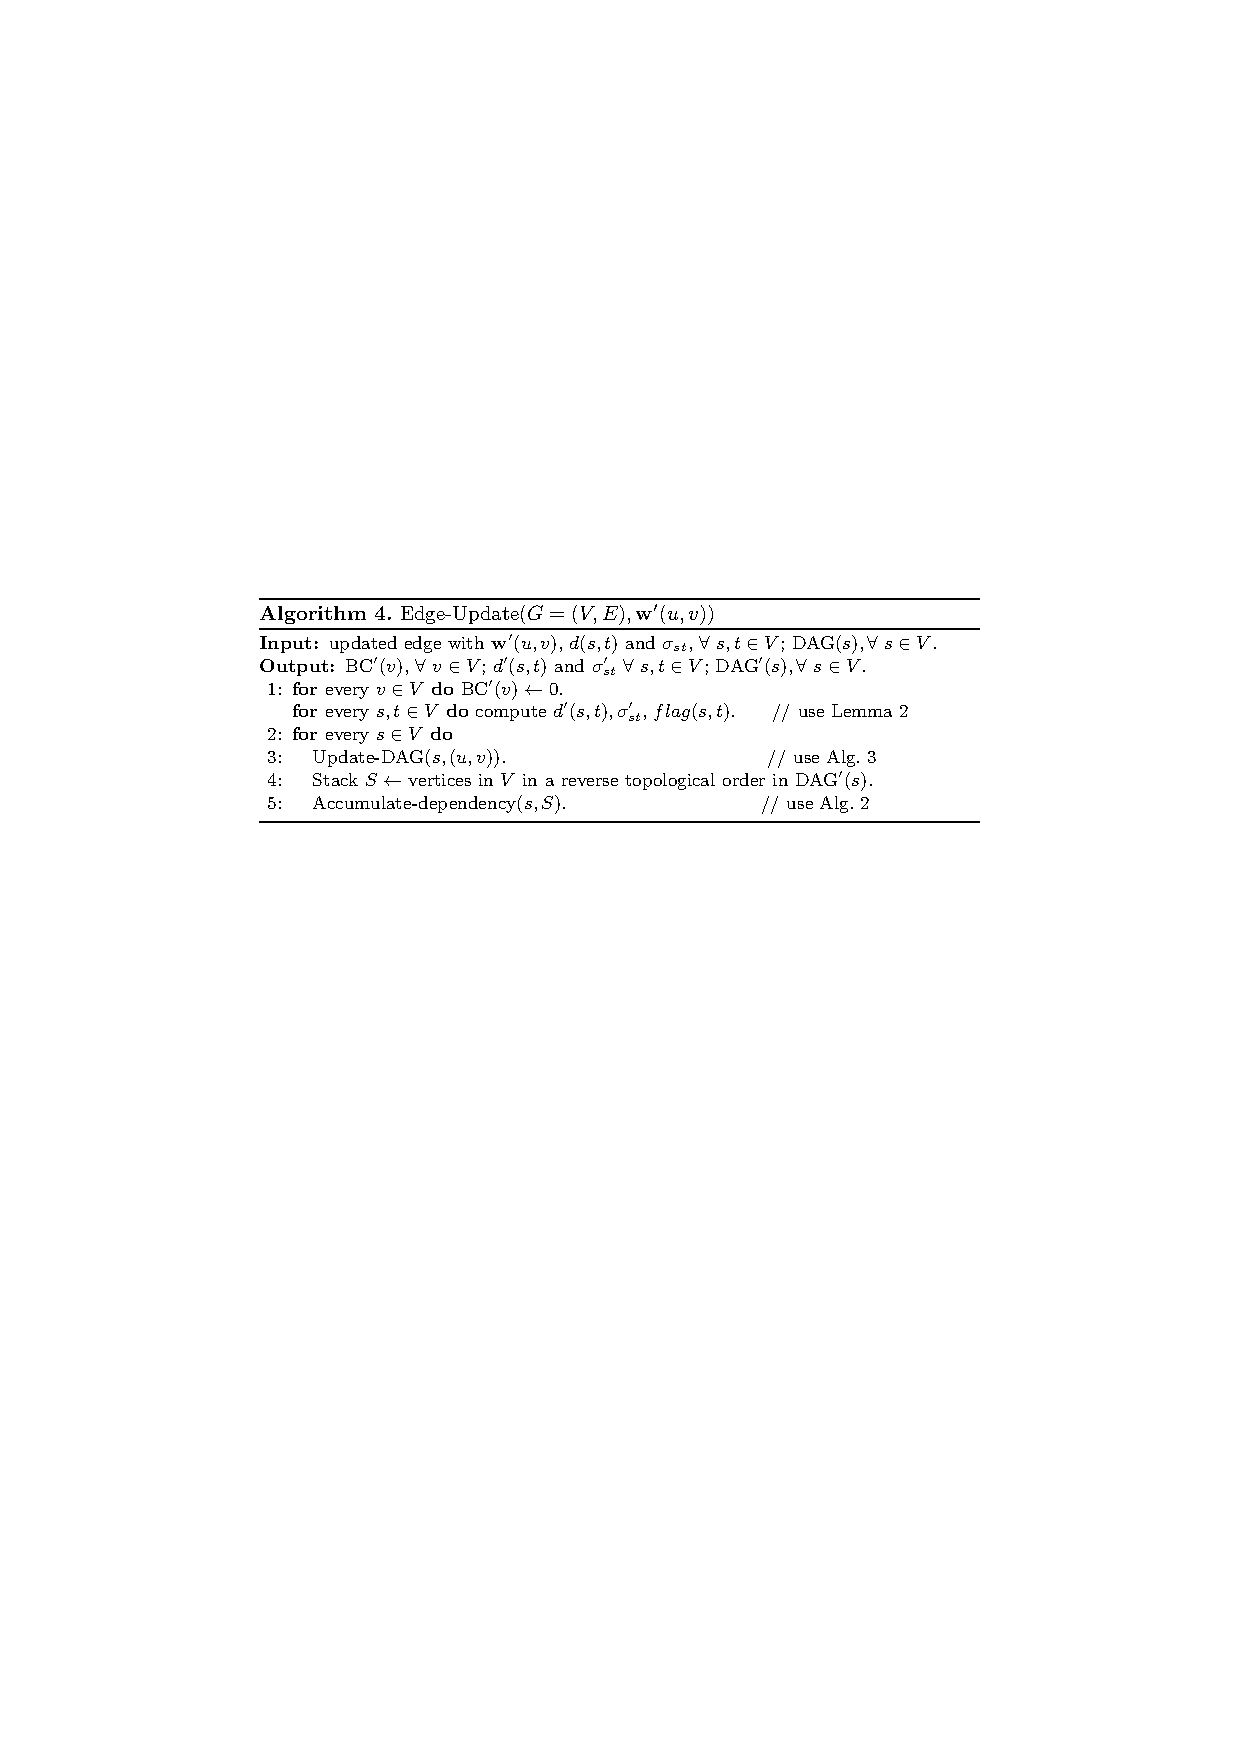
\includegraphics[width=\textwidth]{imgs/npr14-algo4}
  \end{figure}
\end{frame}


\begin{frame}
  \frametitle{Space-Efficient Variant $O(n^2)$}

  \begin{itemize}
    \item Do not store the \spdag
    \item Store only $E^*$
    \item Updated \spdag can be build in $O(m^*)$ time
      \begin{itemize}
        \item Time $O(m^* \, n)$
        \item Compute ${E'}^*$ from $E^*$, then $\spdag'_{s}$ from ${E'}^*$
      \end{itemize}
    \item Space $O(m^* + n^2)$ to store $E^*$ and $n^2$ distances $\dist(s,t)$ and shortest paths $\paths_{st}$
  \end{itemize}
\end{frame}


\begin{frame}
  \frametitle{Comparison}

  \begin{figure}[H]
    \centering
    \includegraphics[width=\textwidth]{imgs/npr14-comparison}
  \end{figure}
\end{frame}


\begin{frame}
  \frametitle{Conclusions}

  \begin{itemize}
    \item Provably faster than Brandes' on weighted graphs
    \item However $m^*$ can be large in practice
    \item No experiments
    \item Hard to parallelize (need to access pairs of \spdag at a time)
    \item Still has main bottleneck of most algorithms: $O(n^2)$ memory
  \end{itemize}
\end{frame}


%% Sariyuce et al. (incremental closeness)
\begin{frame}
  \centering
  \vfill
  {\huge Incremental Algorithms for Closeness Centrality}
  \vfill
  {\Large A. E. Sar\i y\"uce, K. Kaya, E. Saule, U.~V.~\c{C}ataly\"urek }
  \vfill
  {\large IEEE BigData '13: International Conference on Big Data}
  \vfill
\end{frame}


\begin{frame}
  \frametitle{Intuition}

  \begin{itemize}
    \item Algorithm with pruning based on level difference (similar to Green et al.)
    \item Additional pruning by bi-connected decomposition (similar to QUBE)
    \item Applied to closeness centrality (still solves APSP)
    \item Reminder: closeness centrality
    \item $\displaystyle c_{\mathrm{clos}}(v)=\frac{1}{\displaystyle  \sum_{u \in V} d(u,v)}$
  \end{itemize}

\end{frame}


\begin{frame}
  \frametitle{Preliminaries}

  \begin{itemize}
    \item Best static algorithm $O(nm)$ time
  \end{itemize}

  \begin{figure}[H]
    \centering
    \includegraphics[width=\textwidth, height=0.7\textheight, keepaspectratio]{imgs/sksc-algo1}
  \end{figure}
\end{frame}


\begin{frame}
  \frametitle{Cases}

  \begin{figure}[H]
    \centering
    \includegraphics[width=\textwidth]{imgs/sksc-cases}
  \end{figure}

  \begin{itemize}
    \item Usual cases: $dd=0$, $dd=1$, $dd>1$
  \end{itemize}
\end{frame}


\begin{frame}
  \frametitle{Pruning - level difference}

  \begin{figure}[H]
    \centering
    \includegraphics[width=\textwidth, height=0.7\textheight, keepaspectratio]{imgs/sksc-algo2}
  \end{figure}
\end{frame}


\begin{frame}
  \frametitle{Pruning - biconnected components}

  \begin{figure}[H]
    \centering
    \includegraphics[width=\textwidth, height=0.5\textheight, keepaspectratio]{imgs/sksc-biconnected}
  \end{figure}

  \begin{itemize}
    \item If graph has articulation points
    \item Change in $A$ can change closeness of any vertex in $B$
    \item It is enough to compute change for $u$ (constant factor is added for the rest of $B$)
  \end{itemize}
\end{frame}


\begin{frame}
  \frametitle{Maintaining biconnected decomposition}

  \begin{figure}[H]
    \centering
    \includegraphics[width=\textwidth, height=0.5\textheight, keepaspectratio]{imgs/sksc-bidecomp}
  \end{figure}

  \begin{itemize}
    \item Assume edge $(b,d)$ added
    \item Similar to QUBE
  \end{itemize}
\end{frame}


\begin{frame}
  \frametitle{\sssp hybridization}

  \begin{itemize}
    \item BFS can be performed in two ways
    \item \emph{Top-down:} process vertices at distance $d$ to find vertices at distance $d+1$
    \item \emph{Bottom-up:} after vertices at distance $d$ are found, process all unprocessed vertices to see if they are neighbors of the frontier
    \item Top-down is better for initial rounds, bottom-up better for final rounds
    \item Hybridization: use best option at each round
  \end{itemize}
\end{frame}


\begin{frame}
  \frametitle{Fraction of cases}

  \begin{figure}[H]
    \centering
    \includegraphics[width=\textwidth, height=0.5\textheight, keepaspectratio]{imgs/sksc-results1}
  \end{figure}

  \begin{itemize}
    \item Probability distribution for level difference $dd$
    \item Most edges are easy cases
  \end{itemize}
\end{frame}

\begin{frame}
  \frametitle{Speedup}

  \begin{figure}[H]
    \centering
    \includegraphics[width=\textwidth, height=0.5\textheight, keepaspectratio]{imgs/sksc-results2}
  \end{figure}

  \begin{itemize}
    \item Speedup of 2 orders of magnitude
    \item Mostly due to level pruning
    \item Biconnected decomposition and hybridization also give good speedups
  \end{itemize}
\end{frame}


%% Kourtellis et al.
\begin{frame}
  \centering
  \vfill
  {\huge Scalable Online Betweenness Centrality in Evolving Graphs}
  \vfill
  {\Large N. Kourtellis, G. De-Francisci-Morales, F. Bonchi}
  \vfill
  {\large TKDE: IEEE Transactions on Knowledge and Data Engineering (2015)}
  \frametitle{Scalable Online Betweenness Centrality in Evolving Graphs}
  \vfill
\end{frame}


\begin{frame}
  \frametitle{Intuition}

  \begin{itemize}
    \item Incremental, exact, space-efficient, out-of-core, parallel version of Brandes'
    \item Handles edge addition and removal
    \item Vertex and edge betweenness
    \item Scalable to graphs with millions of vertices
  \end{itemize}

\end{frame}


\begin{frame}
  \frametitle{Algorithm}

  \begin{itemize}
    \item Run a modified Brandes' on the initial graph
    \item Keep track of \dist, \paths, \dep in a \spdag (no \pred)
    \item On edge update, adjust the \spdag and update \betw
  \end{itemize}

  \begin{figure}[t]
    \centering
    \includegraphics[width=\textwidth, height=0.6\textheight, keepaspectratio]{imgs/kdb-algo}
  \end{figure}

\end{frame}


\begin{frame}
  \frametitle{Data structure}

  \begin{itemize}
    \item $\spdag_s$ for each source $s \in V$
    \item \spdag contains \dist, \paths, \dep for each other vertex $t \in V$
    \item No predecessors \pred, re-scan neighbors and use \dist to find them
      \begin{itemize}
        \item Save memory - space complexity $O(n^2)$
        \item Fixed size data structure - efficient out-of-core management
        \item Same time complexity $O(nm)$ - in practice, makes the algorithm faster
      \end{itemize}
  \end{itemize}

\end{frame}


\begin{frame}
  \frametitle{Pivot}

  \begin{itemize}
    \item When adding or removing an edge, consider $dd = |d_{su} - d_{sv}|$
    \item Three cases: $dd=0$, $dd=1$, $dd>1$ (analogous to Green et al.)
    \item Last case $dd>1$ hardest - structural changes in \spdag
    \item Find \emph{pivots} to discover structural changes
  \end{itemize}

  \begin{definition}[Pivot]
    Let $s$ be the current source, let $\dist$ and $\dist'$ be the distance before and after an update, respectively, we define \emph{pivot} a vertex $p \mid \dist(s,p) = \dist'(s,p) \wedge \exists \, w \in \neighbors(p)$$: \dist(s,w)$$\neq$$\dist'(s,w)$.
  \end{definition}

  \begin{itemize}
    \item Pivots' distance unchanged $\rightarrow$ use as starting points to correct distances
  \end{itemize}

\end{frame}


\begin{frame}
  \frametitle{Finding pivots}

  \begin{itemize}
    \item Addition - pivots in sub-dag rooted in $u_L = v$
    \item vertices moved closer must be reachable from $u_L$
    \item Can be found during exploration while fixing \paths
  \end{itemize}
  \begin{itemize}
    \item Removal - pivots may be anywhere
    \item Need one exploration to find them
    \item Need separate exploration from found pivots to correct distances
  \end{itemize}

  \begin{figure}[t]
    \centering
    \includegraphics[width=\textwidth, height=0.5\textheight, keepaspectratio]{imgs/kdb-bfs}
  \end{figure}

\end{frame}


\begin{frame}
  \frametitle{Structural changes}

  \begin{figure}[t]
    \centering
    \includegraphics[width=\textwidth, height=0.5\textheight, keepaspectratio]{imgs/kdb-cases}
  \end{figure}

  \begin{itemize}
    \item Consider $x \in \neighbors(y)$, $x$ can either be a sibling or a predecessor of $y$
    \item Each case requires slightly different combination of corrections for \dist, \paths, \dep
    \item $y$ is pivot in 1d, 2e, 2f
    \item Removal for case 1d can be optimized (pivot $y$ is sibling of $x$)
  \end{itemize}

\end{frame}


\begin{frame}
  \frametitle{Scalability}

  \begin{itemize}
    \item Out-of-core - stream \spdag from disk
      \begin{itemize}
        \item In-place update on disk to minimize writes
      \end{itemize}
    \item Columnar storage for \dist, \paths, \dep
      \begin{itemize}
        \item Read only \dist, skip rest if $dd=0$
      \end{itemize}
    \item Parallelization - coarse grained over $s$
      \begin{itemize}
        \item Implementation in MapReduce, amenable to Apache Storm/Flink/Spark
      \end{itemize}
  \end{itemize}

\end{frame}


\begin{frame}
  \frametitle{Results}

  \begin{figure}[t]
    \centering
    \includegraphics[width=\textwidth, height=0.6\textheight, keepaspectratio]{imgs/kdb-results1}
    \caption{Speedup over Brandes' on synthetic and real graphs ($n = 10k$)}
  \end{figure}

  \begin{itemize}
    \item In-memory (M-) version faster than out-of-core (D-)
    \item Without predecessor (-O) always faster than with predecessors (-P)
  \end{itemize}

\end{frame}


\begin{frame}
  \frametitle{Results}

  \begin{figure}[t]
    \centering
    \includegraphics[width=\textwidth, height=0.6\textheight, keepaspectratio]{imgs/kdb-results2}
    \caption{Speedup over Brandes' for out-of-core version on synthetic and real graphs ($n = 1M$)}
  \end{figure}

  \begin{itemize}
    \item Out-of-core version scales up to 1M vertices
    \item Speedup up to 2 orders of magnitude
  \end{itemize}

\end{frame}

\begin{frame}
  \frametitle{Conclusions}

  \begin{itemize}
    \item Fully dynamic (addition and removal)
    \item Algorithm can scale to graphs with realistic size
    \item Ideal horizontal scalability
    \item $O(n^2)$ space bottleneck
  \end{itemize}
\end{frame}

% Contains
%   - Exact algorithms on static graphs (including GPU)
%   - Exact algorithms on dynamic graphs (including streaming/parallel)
% Contains
%   - Scalable algorithms (e.g., GPU)
\section{Approximation Algorithms}
\begin{frame}
  \frametitle{Outline}
  \begin{itemize}
    \item XXX
  \end{itemize}
\end{frame}

\subsection{Approximation Algorithms for Static Graphs}

\begin{frame}
  \centering
  \vfill
  {\huge Fast approximation of centrality}
  \vfill
  {\Large D.~Eppstein, J.~Wang}
  \vfill
  {\large Journal of Graph Algorithms and Applications (2004)}
  \vfill
\end{frame}

\begin{frame}
  \centering
  \vfill
  {\Huge Centrality Estimation in Large Networks}
  \vfill
  {\Large U.~Brandes, C.~Pich}
  \vfill
  {\large International Journal of Bifurcation and Chaos (2007)}
  \vfill
\end{frame}

\begin{frame}
  \centering
  \vfill
  {\huge Better Approximation of Betweenness Centrality}
  \vfill
  {\Large R.~Geisberger, P.~Sanders, D.~Schultes}
  \vfill
  {\large ALENEX (2008)}
  \vfill
\end{frame}

\begin{frame}
  \centering
  \vfill
  {\huge Fast Approximation of Betweenness Centrality through Sampling}
  \vfill
  {\Large M.~Riondato, E.~M.~Kornaropoulos}
  \vfill
  {\large DMKD: Data Mining and Knowledge Discovery (2015)}
  \vfill
\end{frame}

\begin{frame}
  \frametitle{What vertices in a graph are important?}
  Betweenness centrality is one measure of vertex importance\\
  \quad Roughly, it is the fraction of Shortest Paths (SP) in a graph that go through a vertex
  \vfill
  Let $G=(V,E)$, $|V|=n$, $|E|=m$. The betweenness centrality of $v\in V$ is:
  \[
    \betw(v)=\underbrace{\frac{1}{n(n-1)}}_{\mbox{normalization}}\sum_{p_{uw}\in\mathbb{S}_G}
    \underbrace{\frac{\mathds{1}_{\mathcal{T}_v}(p_{uw})}{\sigma_{uw}}}_{\in [0,1]}
  \]
  where:
  \begin{itemize*}
    \item $\mathbb{S}_G$: set of all SPs in $G$
    \item $\mathcal{S}_{uw}$: set of all SPs from $u$ to $w$
      ($\mathcal{S}_{uw}\subseteq\mathbb{S}_G$,
      $|\mathcal{S}_{uw}|=\sigma_{uw}$)
    \item $\mathcal{T}_v$: $\{p\in\mathbb{S}_G ~:~ v\in\mathsf{Int}(p)\}$
  \end{itemize*}
\end{frame}

\begin{frame}
  \frametitle{How to compute betweenness centrality?}
  Na\"ive algorithm: All Pairs SP computation, followed by aggregation\\
  \quad Aggregation dominates runtime, $\Theta(n^3)$
  \vfill
  [Brandes 2001]: Perform aggregation after each Single-Source SP (SSSP) computation\\
  \quad Runtime: $O(nm)$ (unweighted $G$), $O(nm + n^2\log n)$ (weighted
  $G$)\\
  This is is still too much for graphs with $n=10^9$, $m=10^10$
  \vfill
  Possible solution: perform fewer SPs computations by sampling\\
  \quad We get approximate results, but that's OK!
  \vfill
  What kind of approximation do we want ? What should we sample and how much?
\end{frame}

\begin{frame}
  \frametitle{What kind of approximation do we want?}
  We want uniform quality guarantees on the approximations of all vertices
  \vfill
  Definition:\\
  \quad For $\varepsilon,\delta\in(0,1)$, an $(\varepsilon,\delta)$-approximation is
  a collection $\{\tilde{\betw}(v), v\in V\}$ such that
  \[
    \Pr(\exists v\in V ~:~ |\tilde{\betw}(v) -\betw(v)|>\varepsilon)<\delta
  \]
  $\varepsilon$ controls the accuracy, $\delta$ controls the confidence
  \vfill
  Trade-off: smaller $\varepsilon$ or $\delta$ $\Rightarrow$ higher number of
  samples $\Rightarrow$ slower runtime
\end{frame}

\begin{frame}
  \frametitle{How can one get an $(\varepsilon,\delta)$-approximation?}
  [Brandes and Pich, 2008]: only run SSSP and aggregation from a few sources
  \vfill
  \begin{algorithm}[H]
    \DontPrintSemicolon
    $r\leftarrow \frac{1}{\varepsilon^2}\left(\ln n + \ln 2 +
    \ln\frac{1}{\delta}\right)$ \texttt{// sample size}\;
    $\tilde{\betw}(v)\leftarrow 0$, for all $v\in V$\;
    \For(\texttt{// the exact algorithm would iterate over $V$}){$i\leftarrow 1,\dotsc,r$} {
      $v_i \leftarrow$ random vertex from $V$, chosen uniformly\;
      Perform single-source SP computation from $v_i$\;
      Perform partial aggregation, updating $\tilde{\betw}(u)$, $u\in V$,
      like in exact algorithm\;
    }
    Output $\{\tilde{\betw{v}}, v\in V\}$\;
  \end{algorithm}
  \vfill
  Theorem: The output is an $(\varepsilon,\delta)$-approximation
\end{frame}

\begin{frame}
  \frametitle{How do they prove it?}
  Start with bounding the deviation for a single vertex $v$ (Hoeffding bound):
  \[
    \Pr(|\tilde{\betw}(v)-\betw(v)|>\varepsilon)\le 2e^{-2r\varepsilon^2}
  \]
  \vfill
  Then take the union bound over $n$ vertices to ensure uniform converge\\
  \quad the sample size $r$ must be such that
  \[
    2e^{-2r\varepsilon^2}\le\frac{\delta}{n}
  \]
  That is, to get an $(\varepsilon,\delta)$-approximation, we need
  \[
    r\ge\frac{1}{2\varepsilon^2}\left(\ln n + \ln 2 +
    \ln\frac{1}{\delta}\right)
  \]
\end{frame}

\begin{frame}
  \frametitle{What is wrong with this approach?}
  1) We need
  \[
    r\ge\frac{1}{2\varepsilon^2}\left(\ln n + \ln 2 +
    \ln\frac{1}{\delta}\right)
  \]
  \begin{itemize}
    \item This is loose, due to the union bound and does not scale well (experiments)
    \item The sample size depends on $\ln n$. This is not the right
      quantity: not all graphs of $n$ nodes are equally ``difficult'': e.g., the $n$-star is ``easier'' than a random graph
  \end{itemize}
  The sample size $r$ should depend on a more-specific characteristic of the graph
  \vfill
  2) At each iteration, the algorithm performs a SSSP computation\\
  \quad Full exploration of the graph, no locality
\end{frame}

\begin{frame}
  \frametitle{How can we improve the sample size?}
  [R. and Kornaropoulos, 2014] present an algorithm that:
  \vfill
  1) uses a sample size which depends on the vertex-diameter, a characteristic
  quantity of the graph. The derivation uses VC-dimension
  \vfill
  2) samples SPs according to a specific, non-uniform distribution over
  $\mathbb{S}_G$. For each sample, it performs a single $s-t$ SP computation
    \begin{itemize}
      \item More locality: fewer edges touched than single-source SP
      \item Can use bidirectional search / A\textsuperscript{*},
        \ldots
      \end{itemize}
\end{frame}

\begin{frame}
  \frametitle{What is the algorithm?}
  \begin{algorithm}[H]
    \DontPrintSemicolon
    $\mathsf{VD}(G)\leftarrow$ vertex-diameter of $G$ \texttt{// stay
    tuned!}\;
    $r\leftarrow\frac{1}{2\varepsilon^2}\left(\lfloor\log_2(\mathsf{VD}(G)-2\rfloor)
    +1 + \ln(1/\delta)\right)$ \texttt{// sample size}\;
    $\tilde{\betw}(v)\leftarrow 0$, for all $v\in V$\;
    \For{$i\leftarrow 1\dotsc,r$}{
      $(u,v)\leftarrow$ random pair of different vertices, chosen
      uniformly\;
      $\mathcal{S}_{uv}\leftarrow$ all SPs from $u$ to $v$ \texttt{//
      Dijkstra, trunc.~BFS, \ldots}\;
      $p\leftarrow$ random element of $\mathcal{S}_{uv}$, chosen
      uniformly \texttt{// not uniform over $\mathbb{S}_G$}\;
      $\tilde{\betw}(w)\leftarrow \tilde{\betw}(w) + 1/r$, for all
      $w\in\mathsf{Int}(p)$ \texttt{// update only nodes along $p$}\;
    }
    Output $\{\tilde{\betw}(v), v\in V\}$
  \end{algorithm}
  Theorem: The output $\{\tilde{\betw}(v), v\in V\}$ is an
  $(\varepsilon,\delta$)-approximation
\end{frame}

\begin{frame}
  \frametitle{How can we prove the correctness?}
  We want to prove that the output $\{\tilde{\betw}(v), v\in V\}$ is an
  $(\varepsilon,\delta$)-approximation
  \vfill
  Let's apply the recipe!

  \begin{enumerate}
    \item  Define betweenness centrality computation as a expectation
      estimation problem (domain $\domain$, family $\family$, distribution
      $\prob$)
    \item Show that the algorithm efficiently samples according to $\prob$
    \item Show how to efficiently compute an upper bound to the VC-dimension\\
      \quad Bonus: show tightness of bound
    \item Apply the VC-dimension sampling theorem
  \end{enumerate}
\end{frame}

\begin{frame}
  \frametitle{How to define the expectation estimation task?}
  \begin{itemize}
    \item The domain $\domain$ is $\mathbb{S}_G$ (all SPs in $G$)\\
    \item The family is $\family=\{\mathds{1}_{\mathcal{T}_v}, v\in V\}$,
      where $\mathcal{T}_v=\{p\in\mathbb{S}_G ~:~: v\in\mathsf{Int}(p)\}$
    \item The probability distribution $\prob$ on $\domain$ is
      \[
        \pi(p_{uw})=\frac{1}{n(n-1)}\frac{1}{\sigma_{uw}}
      \]
      The algorithm samples paths according to $\pi$
  \end{itemize}
  \vfill
  We have
  \[
    \expectation_\pi[\mathds{1}_{\mathcal{T}_v}]=\sum_{p_{uw}\in\mathbb{S}_G}\mathds{1}_{\mathcal{T}_v}\pi(p_{uw})=\sum_{p_{uw}\in\mathbb{S}_G}\mathds{1}_{\mathcal{T}_v}(p_{uw})\frac{1}{n(n-1)}\frac{1}{\sigma_{uw}}=\betw(v)
  \]
\end{frame}

\begin{frame}
  \frametitle{How do we bound the VC-dimension?}
  Definition: The vertex-diameter $\mathsf{VD}(G)$ of $G$ is the maximum
  number of vertices in a SP of $G$
  \[
    \mathsf{VD}(G)=\max\{|p|, p\in\mathbb{S}_G\}
  \]
  If $G$ is unweighted, $\mathsf{VD}(G)=\Delta(G)+1$. Otherwise no relationship\\
  Very small in social networks, even huge ones (shrinking diameter effect)
  \vfill
  Computing $\mathsf{VD}(G)$: $\left(2\frac{\mbox{max.~edge weight}}{\mbox{min.~edge
  weight}}\right)$-approximation via single-source SP
  \vfill
  Theorem: The VC-dimension of $(\mathbb{S}_G,F)$ is at most $\lfloor\log_2\mathsf{VD}(G)
  -2\rfloor +1$
\end{frame}

\begin{frame}
  \frametitle{Let's prove it!}
  Theorem: The VC-dimension is at most $\lfloor\log_2\mathsf{VD}(G)
  -2\rfloor +1$
  \vfill
  Proof:
  \begin{itemize}
    \item For a set $A\subseteq\mathbb{S}_G$ of size $|A|=d$ to be
      shattered, any $p$ in $A$ must appear in at least $2^{d-1}$
      different sets $\mathcal{T}_v$, one for each subset of $A$
      containing $p$.
    \item Any $p$ appears only in the sets $\mathcal{T}_v$ such that
      $v\in\mathsf{Int}(p)$\\
      \quad There are $|\mathsf{Int}(p)|$ such sets
    \item From the definition of the vertex-diameter $\mathsf{VD}(G)$, we have
      $|\mathsf{Int}(p)|\le\mathsf{VD}(G)-2$
    \item To shatter $A$, $d$ must be such that $2^{d-1}\le\mathsf{VD}(G)-2$
    \item So $d$ can be at most $\lfloor\log_2\mathsf{VD}(G) -2\rfloor +1$,
      otherwise $A$ can not be shattered
  \end{itemize}
\end{frame}

\begin{frame}
  \frametitle{How to use the bound?}
  We have that:
  \begin{itemize}
    \item The estimation $\tilde{\betw}(v)$ computed by the algorithm is the
      empirical average for $\betw(v)$
    \item The algorithm samples SPs efficiently according to $\prob$
    \item We know an upper bound to the VC-dimension and how to compute it
      efficiently
  \end{itemize}
  Thus we can apply the VC $\varepsilon$-sample theorem, and obtain that the algorithm
  outputs an $(\varepsilon,\delta)$-approximation:
  \[
    \Pr(\exists v\in V ~:~ |\tilde{\betw}(v)-\betw(v)|>\varepsilon)<\delta
  \]
\end{frame}

\begin{frame}
  \frametitle{Is the bound to the VC-dimension tight?}
  Yes! There is a class of graphs with VC-dimension exactly
  $\lfloor\log_2\mathsf{VD}(G) -2\rfloor +1$\\
  \quad The Concertina Graph Class $(G_i)_{i\in\mathbb{N}}$:
  \begin{figure}[H]
    \centering
    \includegraphics[scale=0.3]{imgs/concertina}
  \end{figure}
  \vfill
  Theorem: The VC-dimension of $(\mathbb{S}_{G_i}, F)$ is
  $\lfloor\log_2\mathsf{VD}(G) -2\rfloor +1=i$
  \vfill
  Proof Intuition: The middle vertices are internal to a lot of SPs
\end{frame}

\begin{frame}
  \frametitle{Is the Vertex-Diameter the right quantity?}
  No! If $G$ undirected and for every connected pair of nodes there is a
  unique SP, then the VC-dimension is at most 3\\
  \quad These graphs are not just trees!
  \vfill
  Proof: in such a graph, two SPs that meet and separate can not meet again\\
  \quad (+ multiple case analysis)
  \vfill
  The bound ``3'' is tight. In the following graph we can shatter 3 paths
  \begin{figure}[H]
    \centering
    \includegraphics[scale=0.3]{imgs/uniqueshortestpathtight}
  \end{figure}
  \vfill
  There is room for improvement using pseudodimension (we are working on that!)
\end{frame}

\begin{frame}
  \frametitle{What about directed graphs?}
  Does a similar result also hold for directed graphs with unique SP?\\
  \quad  Not for the same constant $3$. We built a graph with unique SPs between
  all connected nodes and we can shatter a set of $4$ SPs
  \begin{figure}[H]
    \centering
    \includegraphics[scale=0.3]{imgs/uniquedirected}
  \end{figure}
  Yes, finding counterexamples is messy\ldots
  \vfill
  Does it hold for a different constant?\\
  \quad We do not know! Maybe you can work on that?
\end{frame}

\begin{frame}
  \frametitle{How well does the algorithm perform in practice?}
  It performs very well!
  \vfill
  We tested the algorithm on real graphs (SNAP) and on artificial
  Barabasi-Albert graphs, to evalue its accuracy, speed, and scalability
  \vfill
  Results: It blows away the exact algorithm and the union-bound-based
  sampling algorithm
\end{frame}

\begin{frame}
  \frametitle{How accurate is the algorithm?}
  In $O(10^3)$ runs of the algorithm on different graphs and with different
  parameters, we always had $|\tilde{\betw}(v)-\betw(v)|<\varepsilon$ for all
  nodes\\
  \quad Actually, on average $|\tilde{\betw}(v)-\betw(v)|<\varepsilon/8$
  \vfill
  \begin{figure}[H]
    \centering
    \includegraphics[scale=0.22]{imgs/email-Enron-error}
  \end{figure}
\end{frame}

\begin{frame}
  \frametitle{How fast is the algorithm?}
  Approximately 8 times faster than the simple sampling algorithm
  \vfill
  Variable speedup w.r.t. exact algorithm (200x -- 4x), depending on
  $\varepsilon$
  \vfill
  \begin{figure}[H]
    \centering
    \includegraphics[scale=0.22]{imgs/email-Enron-time}
  \end{figure}
\end{frame}

\begin{frame}
  \frametitle{How scalable is the algorithm?}
  Much more scalable than the simple sampling algorithm, because the sample
  size does not depend on $n$
  \vfill
  \begin{figure}[H]
    \centering
    \includegraphics[scale=0.22]{imgs/random-time}
  \end{figure}
\end{frame}

\begin{frame}
  \frametitle{Conclusions (Betweenness Centrality)}
  \vfill
  We showed a sampling algorithm for betweenness centrality approximation that
  gives probabilistic guarantees on the quality of the approximation for all
  the vertices
  \vfill
  The algorithm samples SPs according to a well-defined distribution, and
  the analysis relies on VC-dimension, which is bounded by the Vertex Diameter,
  a characteristic quantity of the graph that is small in real networks
  \vfill
  The use of VC-dimension makes the algorithm much faster and more scalable
  than previous sampling approaches and than the exact algorithm
\end{frame}

\begin{frame}
  \centering
  \vfill
  {\huge ABRA: Approximating Betweennes Centrality in Static and Dynamic
  Graphs with Rademacher Averages}
  \vfill
  {\large M.~Riondato, E.~Upfal}
  \vfill
  {\large arXiv (2016)}
  \vfill
\end{frame}

\subsection{Approximation Algorithms for Dynamic Graphs}

\begin{frame}
  \centering
  \vfill
  {\huge Fully-Dynamic Approximation of Betweenness Centrality}
  \vfill
  {\Large E.~Bergamini, H.~Meyerhenke}
  \vfill
  {\large ESA: European Symposium on Algorithms (2015)}
  \vfill
\end{frame}

\begin{frame}
  \centering
  \vfill
  {\huge Fully Dynamic Betweenness Centrality Maintenance on Massive
  Networks}
  \vfill
  {\Large T.~Hayashi, T.~Akiba, Y.~Yoshida}
  \vfill
  {\large VLDB: Very Large Databases (2016)}
  \vfill
\end{frame}

\begin{frame}
  \centering
  \vfill
  {\huge Incremental Algorithm for Updating Betweenness Centrality in
  Dynamically Growing Networks}
  \vfill
  {\Large M.~Kas, M.~Wachs, K.~M.~Carley, L.~R.~Carley}
  \vfill
  {\large ASONAM (2013)}
  \vfill
\end{frame}

% Contains
%   - Approximation algorithms on static graphs
%   - Approximation algorithms on dynamic graphs
% !TEX root =  centrtutorial.tex
\section{Conclusions}

\begin{frame}
  \frametitle{What we presented}
  \begin{itemize}
    \pause
    \item Brief survey of the most common measures of centrality
    \item Axioms for centrality
    \item Focusing on closeness and betweenness centrality:
      \begin{itemize}
        \item exact algorithms on static graphs (GPU-based)
        \item exact algorithms on dynamic graphs (streaming, distributed)
        \item approximation algorithms for static graphs
        \item approximation algorithms for dynamic graphs
    \end{itemize}
  \end{itemize}
  In each of the above, there are important open questions and directions for
  future work.
\end{frame}

\begin{frame}
  \frametitle{Big Graphs}
  \begin{itemize}
    \pause
    \item \emph{``Big Data''} is a lot of hype and refers to very different
      things depending on the context.
    \pause
    \item However, the unprecedented \emph{volume}, \emph{velocity}, and
      \emph{variety} pose real algorithmic challenges, especially when dealing
      with expressive and complex representations such as graphs.
    \pause
    \item Challenges are opportunities for researchers!
    \pause
    \item \emph{Big graphs require new algorithms}
  \end{itemize}
\end{frame}

\begin{frame}
  \frametitle{Volume requires new algorithms}
  \pause
  \begin{itemize}
    \item  Classic computational complexity:
    \begin{itemize}
      \item Is there a  polynomial time exact algorithm $\mathbf{\rightarrow}$?
        Go for it!
      \item Your problem is \textbf{NP}-Hard $\mathbf{\rightarrow}$ better think
        about approximation algorithms\ldots
    \end{itemize}
  \item Classic computational complexity: polynomial = feasible
  \pause
  \item But is polynomial time really feasible?
    \begin{itemize}
      \item E.g., Brandes algorithm not feasible for $n = 10^9$
    \end{itemize}
  \pause
  \item On big graphs quadratic time is as bad as \textbf{NP}-Hard
  \begin{itemize}
    \item New, finer-grain, complexity theory needed (?)
  \end{itemize}
  \pause
  \item Need for \emph{massively parallel} algorithms, \emph{out-of-core}
    algorithms, \emph{sublinear} algorithms, \emph{approximated} algorithms,
    \emph{randomized} algorithms, etc.
  \end{itemize}
\end{frame}

\begin{frame}
  \frametitle{Velocity requires new algorithms}
  \pause
  \begin{itemize}
    \item  The velocity with which new data keeps \emph{arriving}\ldots
    \pause
    \item \ldots and the velocity with which the information of interest keeps
      \emph{changing}.
    \vfill
    \item In the case of graphs new edges are formed and old edges might
      disappear at very high speed.
    \pause
    \begin{itemize}
      \item How to maintain the centrality score of all vertices continuously
        updated?
    \end{itemize}
    \vfill
    \pause
    \item Velocity requires \emph{streaming} algorithms that only read each data
    point once (or a few time), specialized small-space data structures
    (\emph{sketches}) that maintain basic statistics and can be updated
      on-the-fly, algorithms which are \emph{robust to changes} in the data, etc.
  \end{itemize}
\end{frame}

\begin{frame}
  \frametitle{Variety requires new algorithms}
  \pause
  \begin{itemize}
    \item Variety refers to the \emph{richness of different information types}
      to be mixed in the analysis.
    \vfill
    \pause
    \item Examples in graphs:
      \begin{itemize}
        \pause
        \item Vertices have attributes;
        \pause
        \item Vertices are spatio-temporally localized and keeps moving;
        \pause
        \item Edges have types (colors);
        \pause
        \item Edges have multiple types (a.k.a.~multigraphs, multiplex networks,
          multidimensional networks, etc.);
        \pause
        \item Each edge has associated a time series representing the amount of
          communication (or activity) along the edge per time unit;
        \pause \item ...
      \end{itemize}
    \vfill
    \pause
    \item Semantic richness in the data implies complexity in the knowledge we can
      extract.
    \pause
    \item Applications involving ``multi-structured'' data require the definition
      of \emph{new, ad-hoc, model and patterns} \ldots
    \pause
    \item \ldots and of course, the \emph{algorithms} to extract them,
    \pause
    \item and these new algorithms need to be able to deal with the volume and the
      velocity!
  \end{itemize}
\end{frame}

\begin{frame}
  \frametitle{Big Graphs}
  \begin{itemize}
    \item The \emph{computational complexity} of most existing graph algorithms
      makes them \emph{impractical} in today's networks, which are:
      \begin{itemize}
        \item massive,
        \item information-rich, and
        \item dynamic.
      \end{itemize}
    \item In order to scale graph analysis to \emph{real-world applications} and
      to keep up with their \emph{highly dynamic nature}, we need to
      \emph{devise new approaches} specifically tailored for \emph{modern
        parallel stream processing engines} that run on clusters of
        shared-nothing commodity hardware.
  \end{itemize}
\end{frame}

\begin{frame}
  \frametitle{\bigskip \bigskip  \Huge Thank you!}
  \centering
  \begin{tabular}{c}
    % after \\: \hline or \cline{col1-col2} \cline{col3-col4} ...
    Francesco Bonchi \\  \emph{http://francescobonchi.com} \\ @FrancescoBonchi\\ $\;$ \\
    Gianmarco De Francisci Morales \\ \emph{http://gdfm.me} \\  @gdfm7\\  $\;$ \\
    Matteo Riondato \\ \emph{http://matteo.rionda.to} \\ @teorionda\\  $\;$ \\
  \end{tabular}
  \begin{block}{\centering Slides available at}
    \centering  http://matteo.rionda.to/centrtutorial/
  \end{block}
\end{frame}

% Contains
%   - Conclusions

%\bibliographystyle{abbrvnat}
%\bibliography{../proceedings/centrality.bib}

\end{document}
